\documentclass[a4paper]{article}
\usepackage{graphicx}
\usepackage{xcolor}
\usepackage{hyperref}
\usepackage{caption}
\usepackage{fancyhdr}
\usepackage{titlesec}

% Define custom colors
\definecolor{titlecolor}{HTML}{4B6EAF}
\definecolor{sectioncolor}{HTML}{287233}
\definecolor{subsectioncolor}{HTML}{FF4500}
\definecolor{linkcolor}{HTML}{1E90FF}

% Set the color of the links
\hypersetup{
    colorlinks=true,
    linkcolor=linkcolor,
    urlcolor=linkcolor
}

% Fancy header and footer
\pagestyle{fancy}
\fancyhf{}
\fancyhead[L]{\textit{Triple Boot Guide: Windows 11, Arch Linux, Ubuntu}}
\fancyhead[R]{Tazmeen Afroz}
\fancyfoot[C]{\thepage}

% Custom title and section styles
\titleformat{\section}
  {\color{sectioncolor}\Large\bfseries}
  {\thesection}{1em}{}
\titleformat{\subsection}
  {\color{subsectioncolor}\large\bfseries}
  {\thesubsection}{1em}{}

% Title information
\title{\textcolor{titlecolor}{\textbf{Triple Boot Installation Guide: Windows 11, Arch Linux, and Ubuntu}}}
\author{Tazmeen Afroz}
\date{\today}

\begin{document}

\maketitle
\begin{center}
    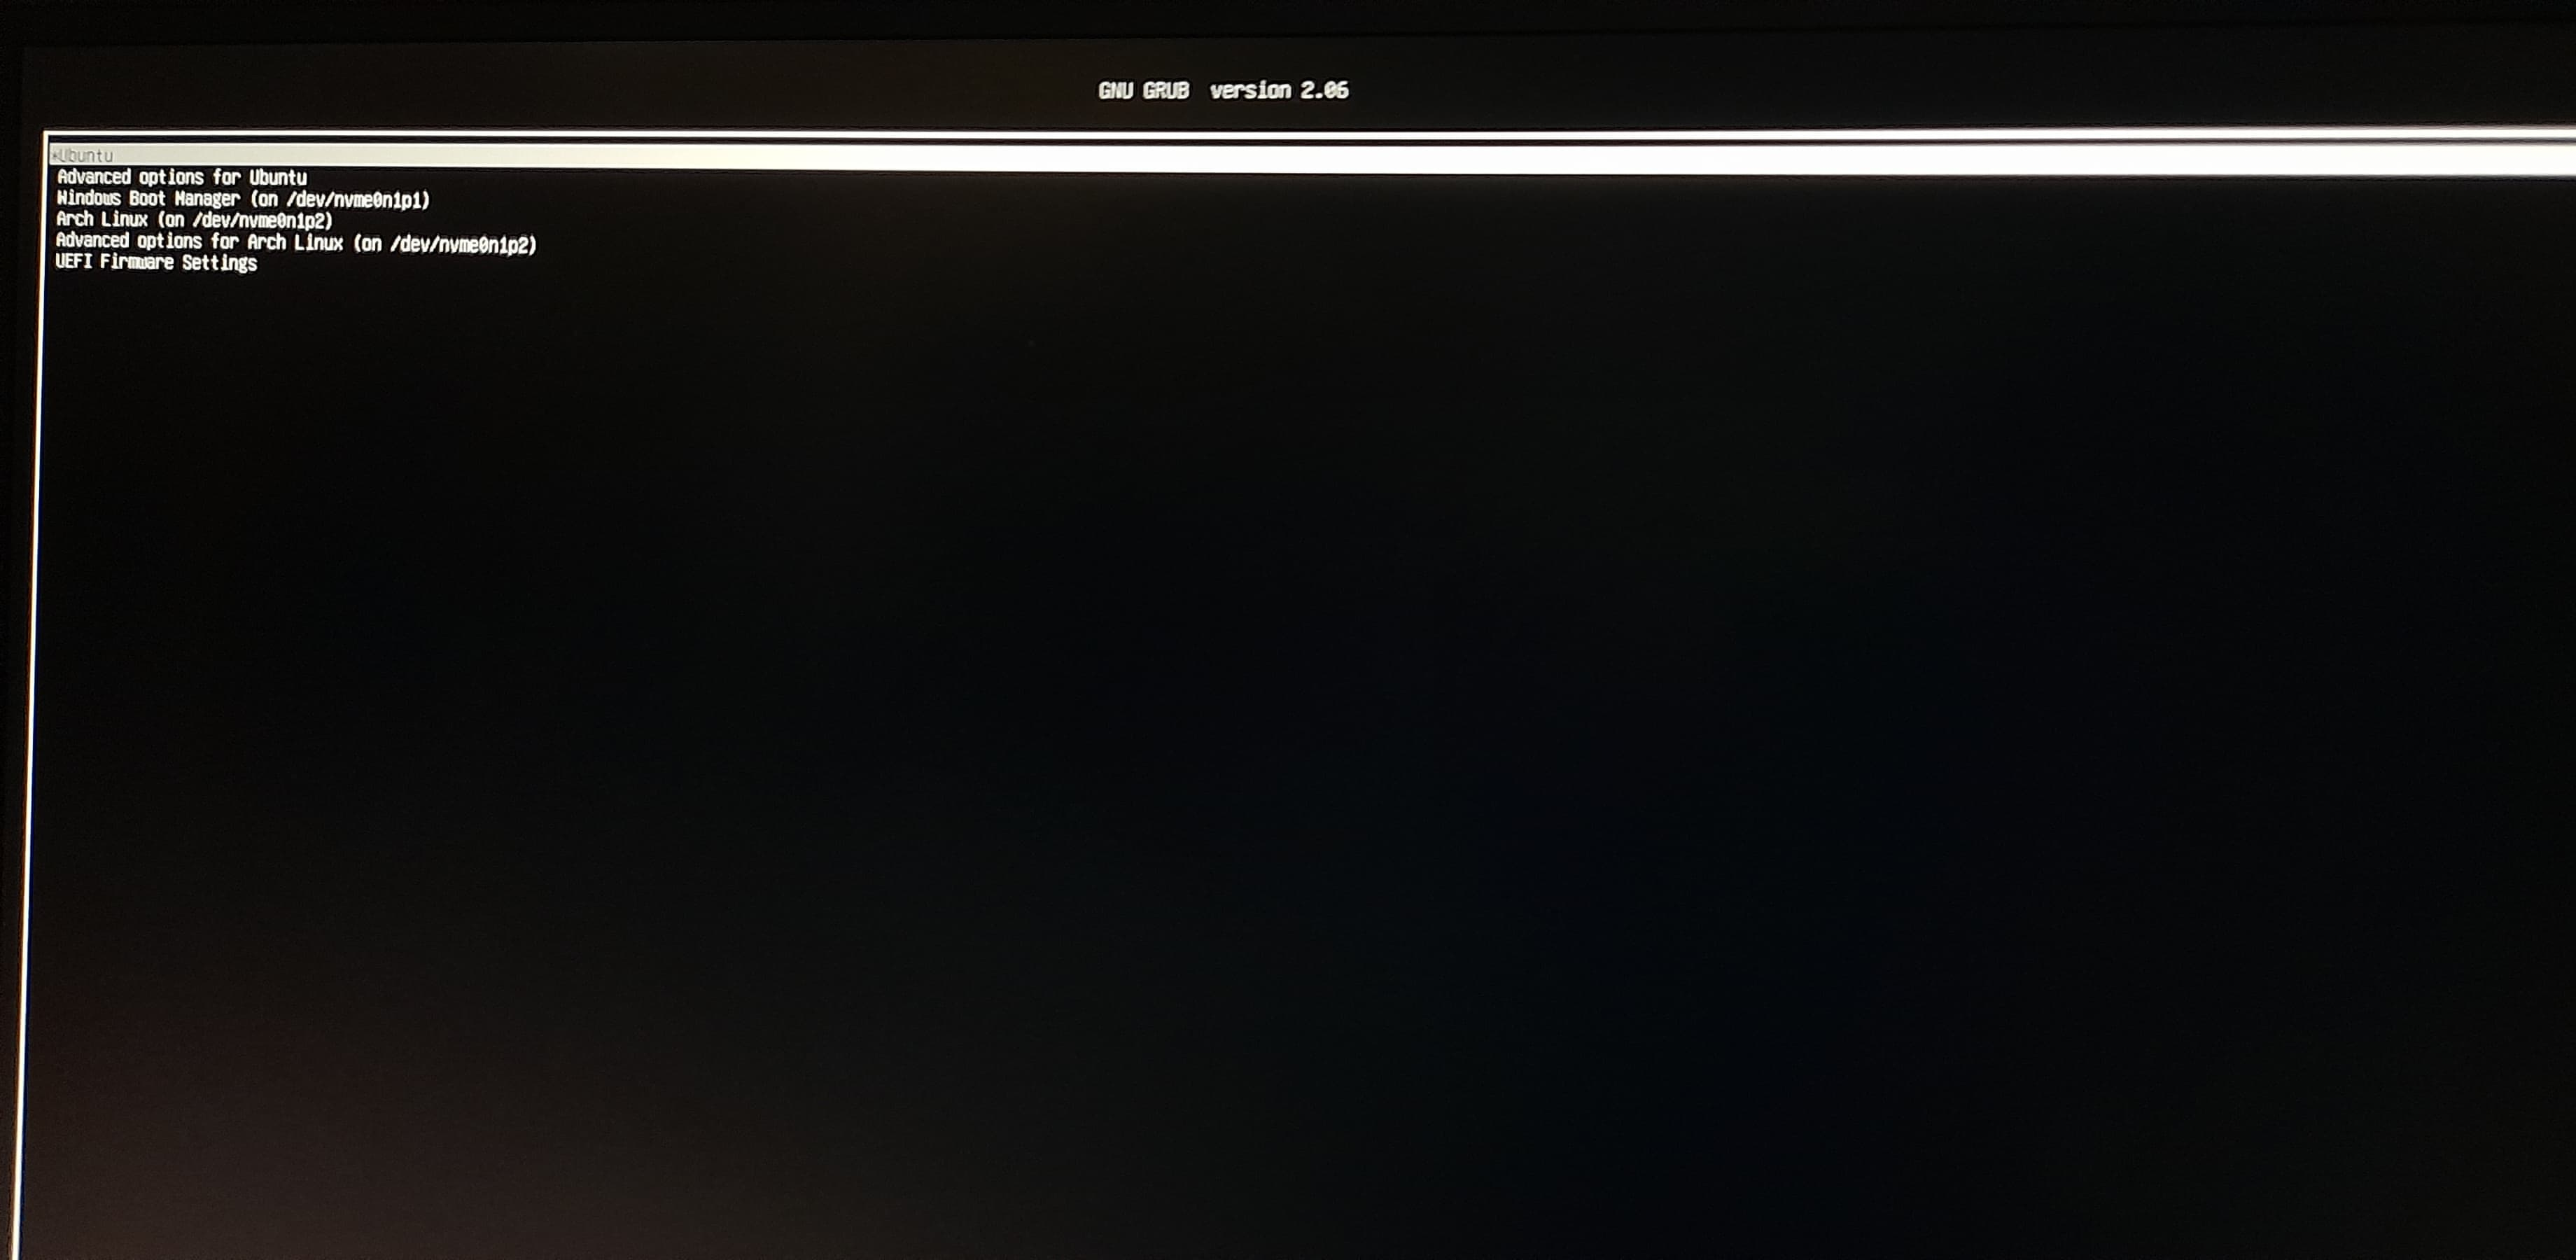
\includegraphics[width=0.8\textwidth]{0.jpeg} % Placeholder for GRUB menu screenshot
    \captionof{figure}{GRUB Menu with Triple Boot Options}
\end{center}
\begin{center}
    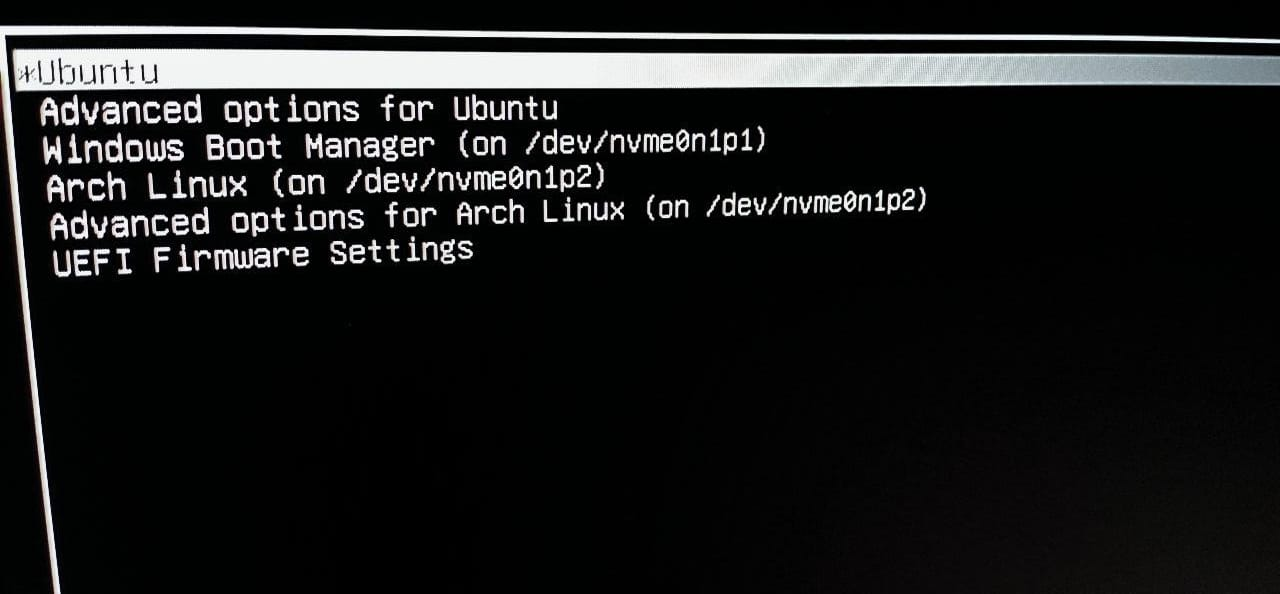
\includegraphics[width=0.8\textwidth]{1.jpeg} % Placeholder for GRUB menu screenshot
    \captionof{figure}{GRUB Menu with Triple Boot Options}
\end{center}


\newpage
\tableofcontents
\newpage

\section{Introduction}
This document provides a comprehensive, step-by-step guide to installing Windows 11, Arch Linux, and Ubuntu on a single machine using a virtual machine setup. The guide covers partitioning, operating system installations, bootloader configurations, and post-installation verification.

\section{Virtual Machine Setup}
We begin by allocating the appropriate resources for the virtual machine, ensuring optimal performance.

\subsection{Disk and RAM Allocation}
Allocate 120GB of disk space and configure the virtual machine with 6784MB of RAM for smooth operation.

\begin{center}
    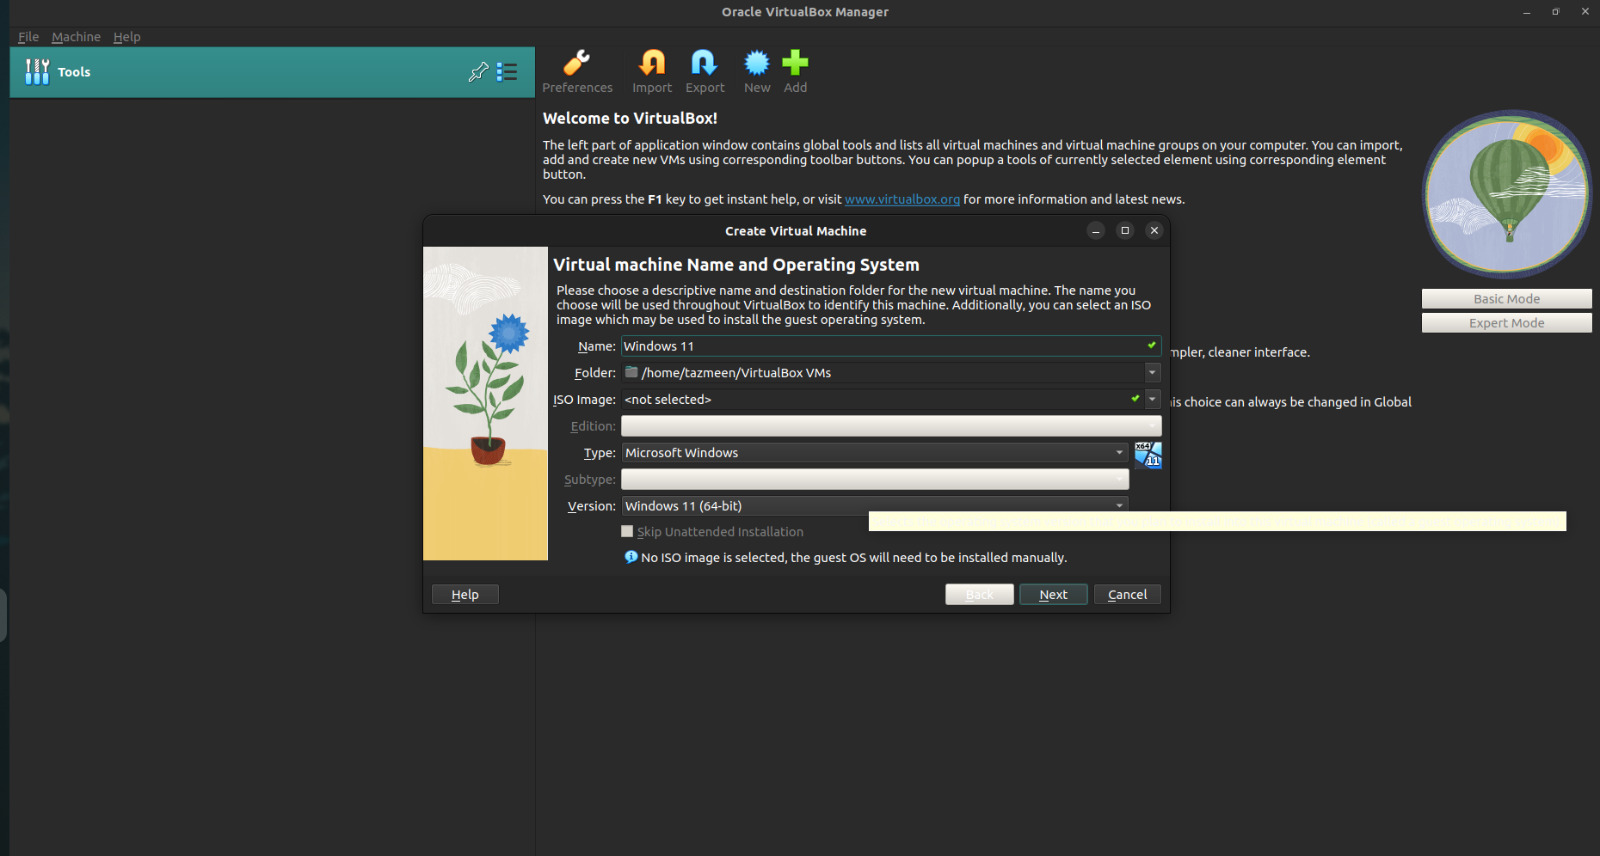
\includegraphics[width=0.8\textwidth]{2.jpeg} % Placeholder for VM allocation screenshot
    \captionof{figure}{Virtual Machine Allocation for Windows, Arch, and Ubuntu}
\end{center}
\begin{center}
    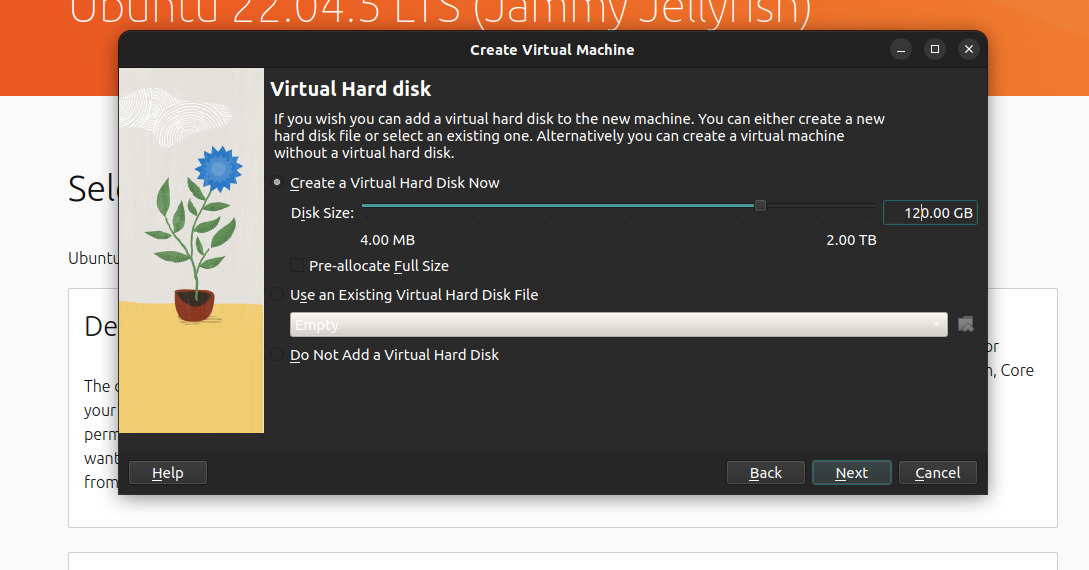
\includegraphics[width=0.8\textwidth]{3.jpeg} % Placeholder for VM allocation screenshot
    \captionof{figure}{Virtual Machine Allocation for Windows, Arch, and Ubuntu}
\end{center}
\begin{center}
    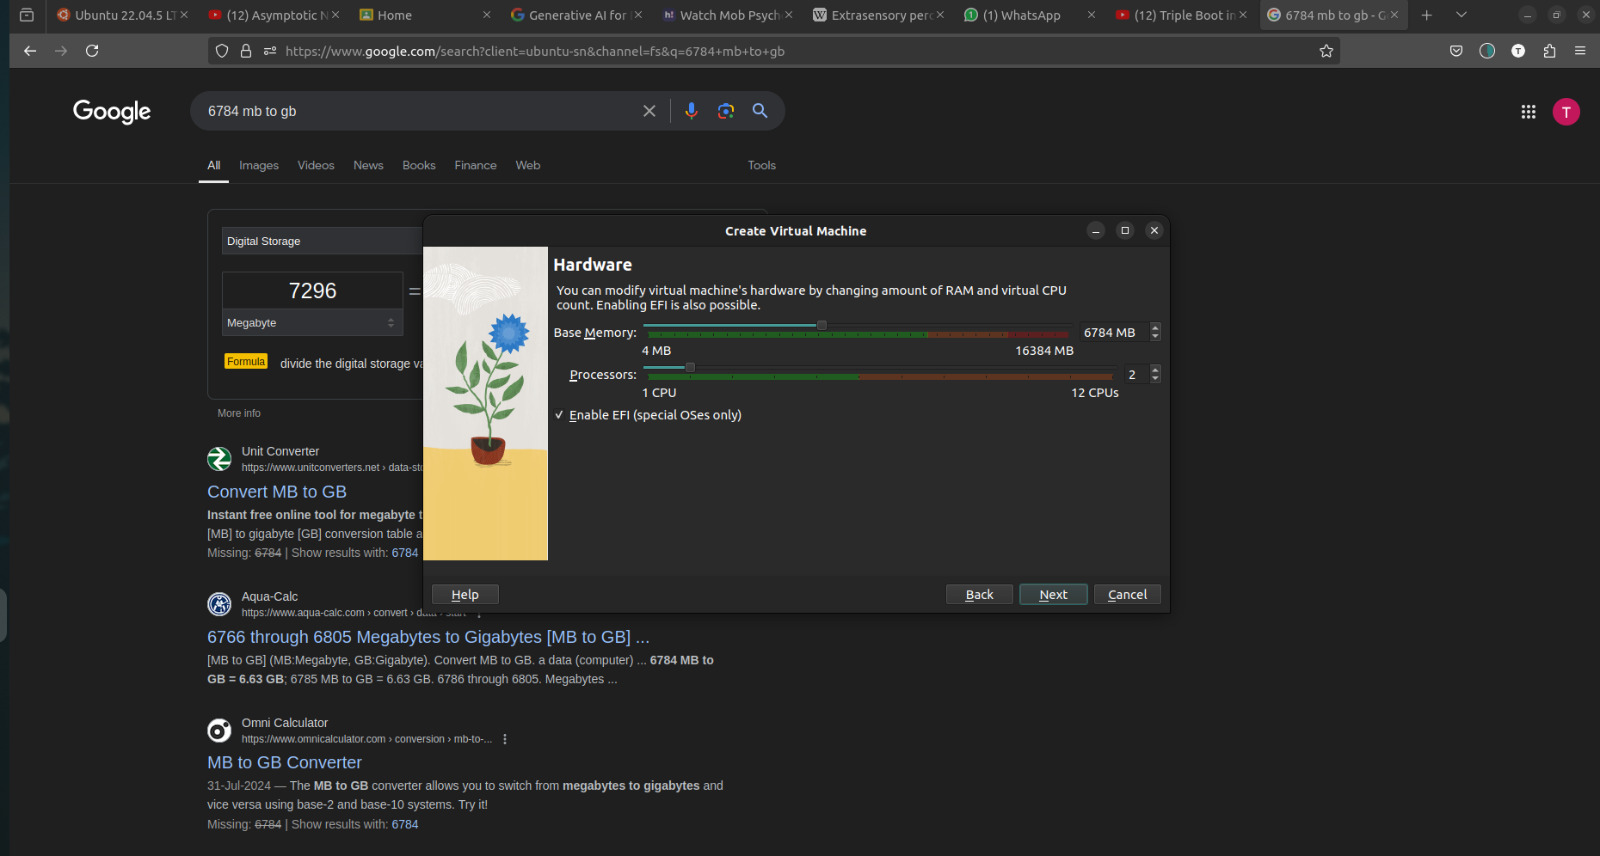
\includegraphics[width=0.8\textwidth]{4.jpeg} % Placeholder for VM allocation screenshot
    \captionof{figure}{Virtual Machine Allocation for Windows, Arch, and Ubuntu}
\end{center}
\begin{center}
    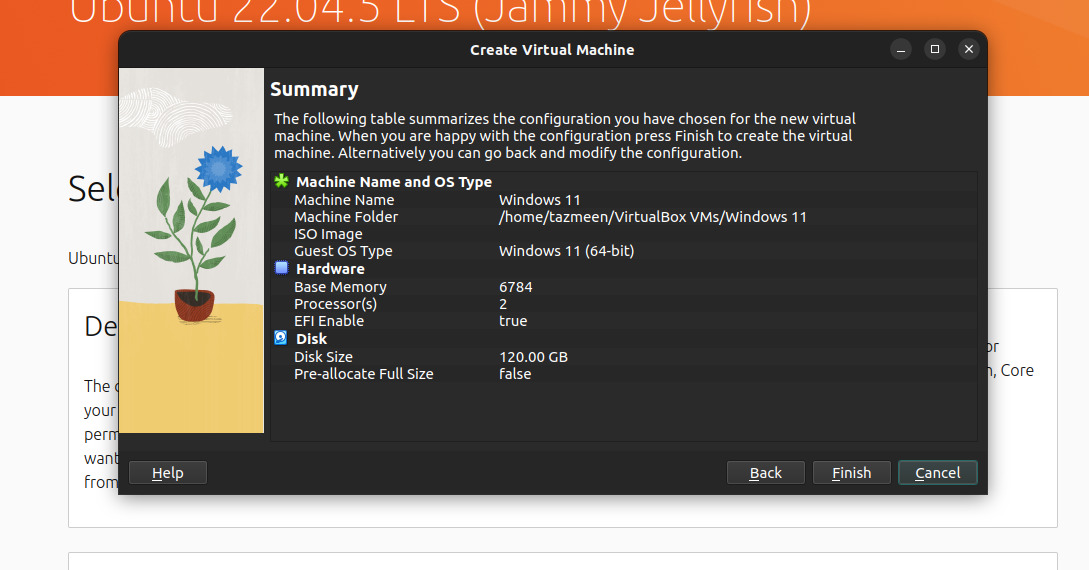
\includegraphics[width=0.8\textwidth]{5.jpeg} % Placeholder for VM allocation screenshot
    \captionof{figure}{Virtual Machine Allocation for Windows, Arch, and Ubuntu}
\end{center}
\begin{center}
    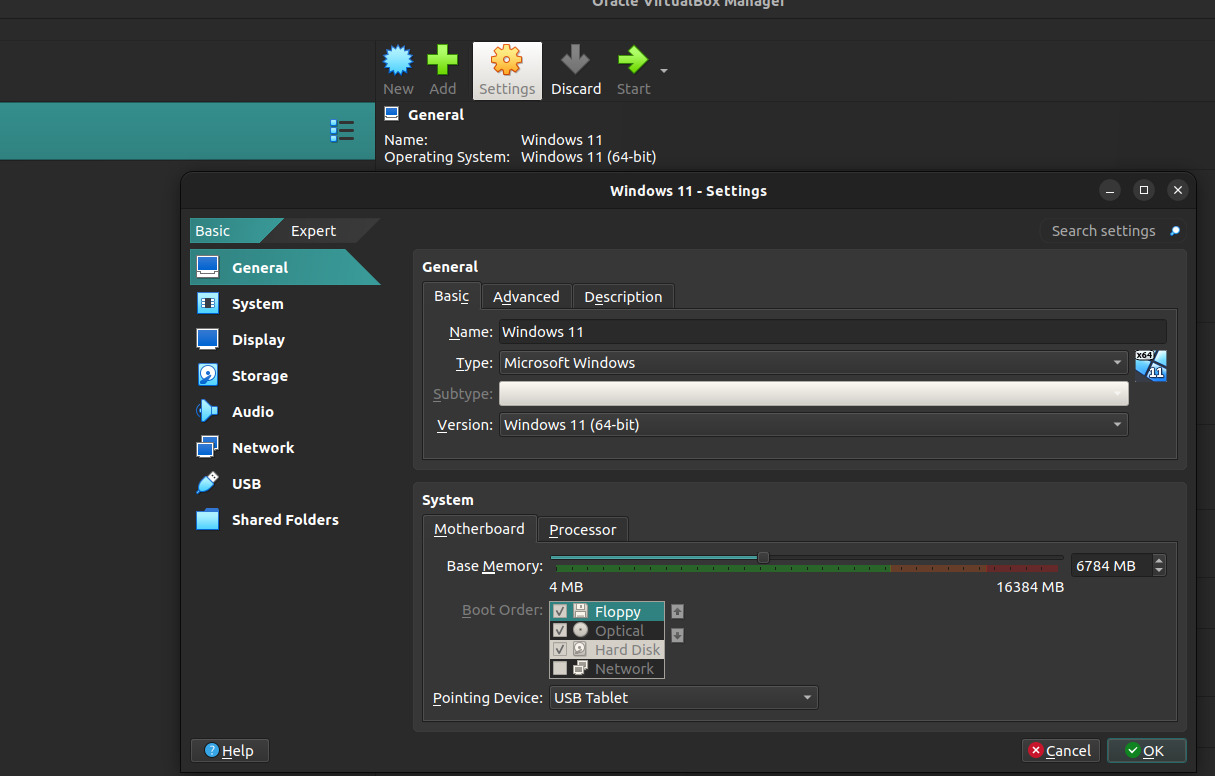
\includegraphics[width=0.8\textwidth]{6.jpeg} % Placeholder for VM allocation screenshot
    \captionof{figure}{Virtual Machine Allocation for Windows, Arch, and Ubuntu}
\end{center}
\begin{center}
    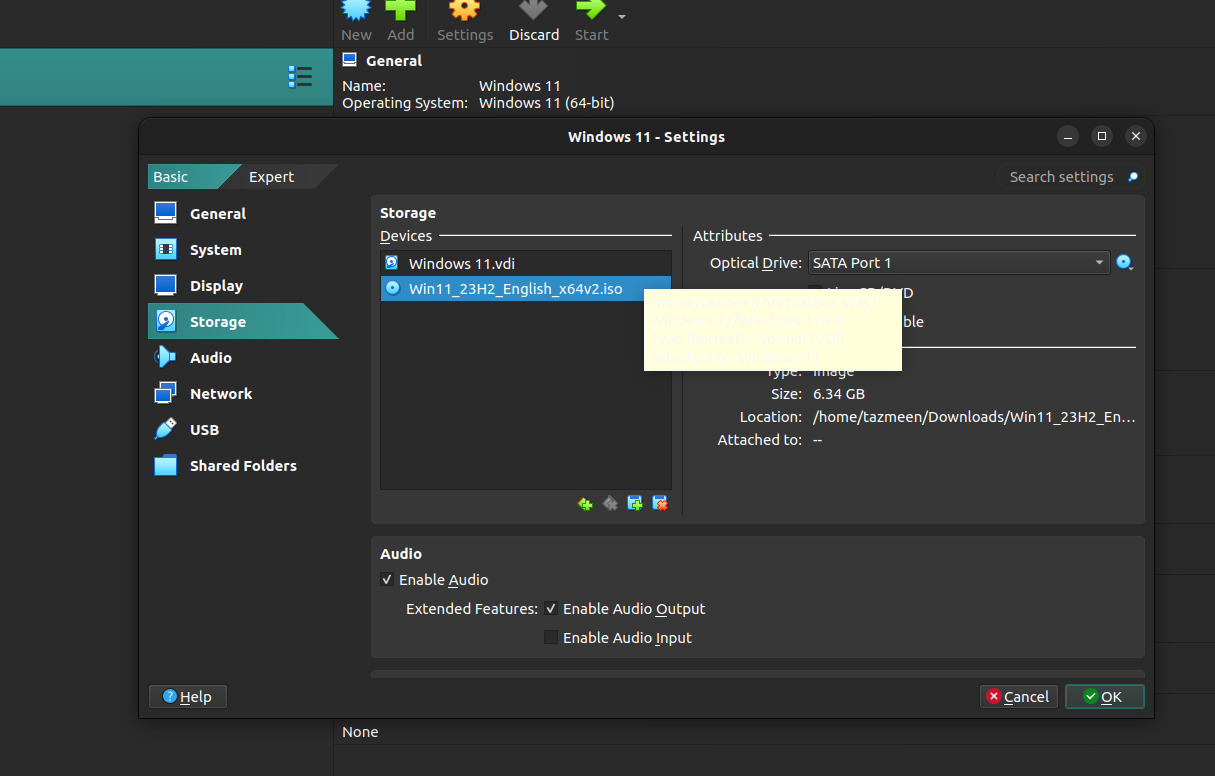
\includegraphics[width=0.8\textwidth]{7.jpeg} % Placeholder for VM allocation screenshot
    \captionof{figure}{Virtual Machine Allocation for Windows, Arch, and Ubuntu}
\end{center}

\section{Installing Windows 11}
Follow the instructions below to install Windows 11 on your virtual machine.

\subsection{UEFI Mode and ISO Selection}
Ensure that the virtual machine is set to UEFI mode, then load the Windows 11 ISO file.

\begin{center}
    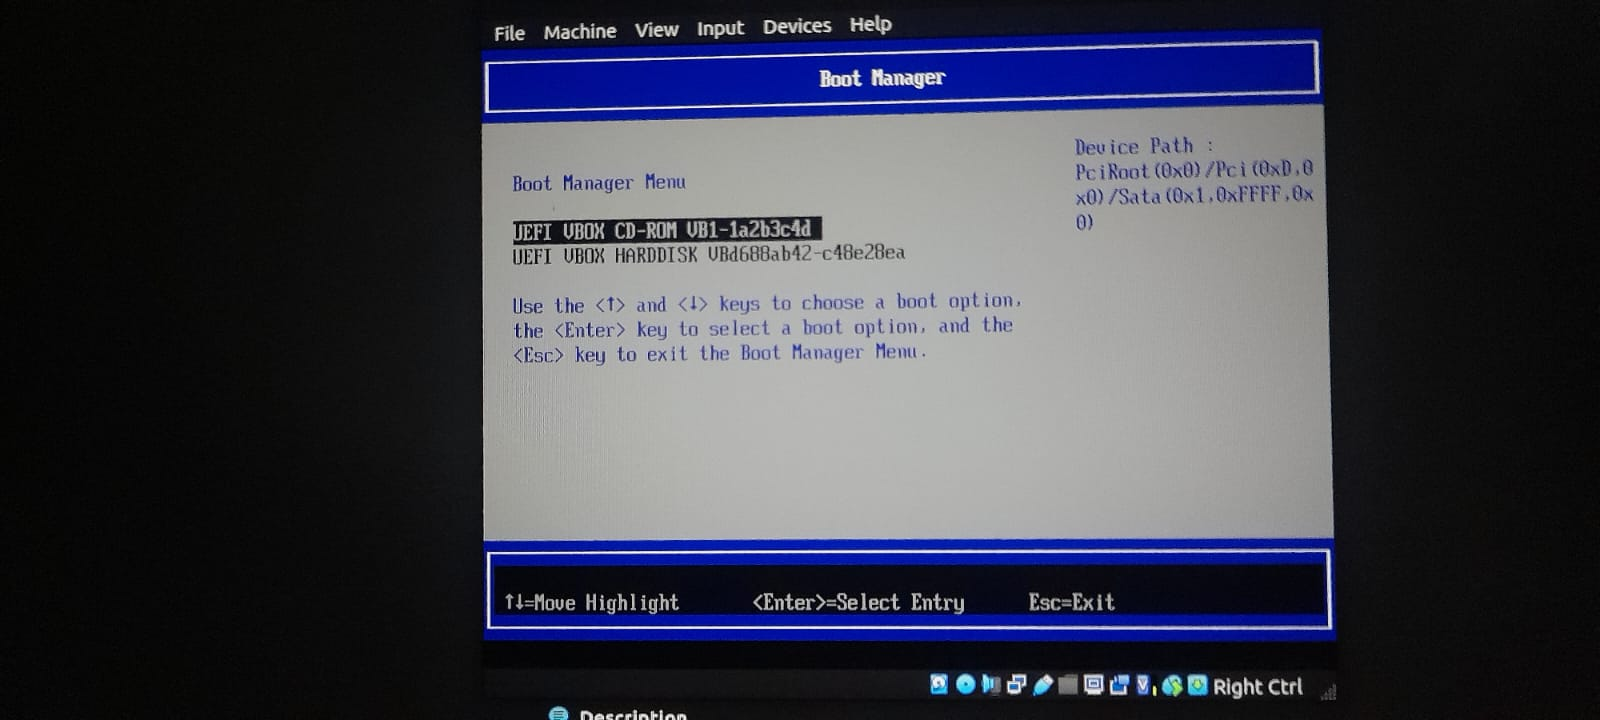
\includegraphics[width=0.8\textwidth]{8.jpeg} % Placeholder for UEFI & ISO screenshot
    \captionof{figure}{Selecting UEFI Mode and Windows ISO File}
\end{center}
\begin{center}
    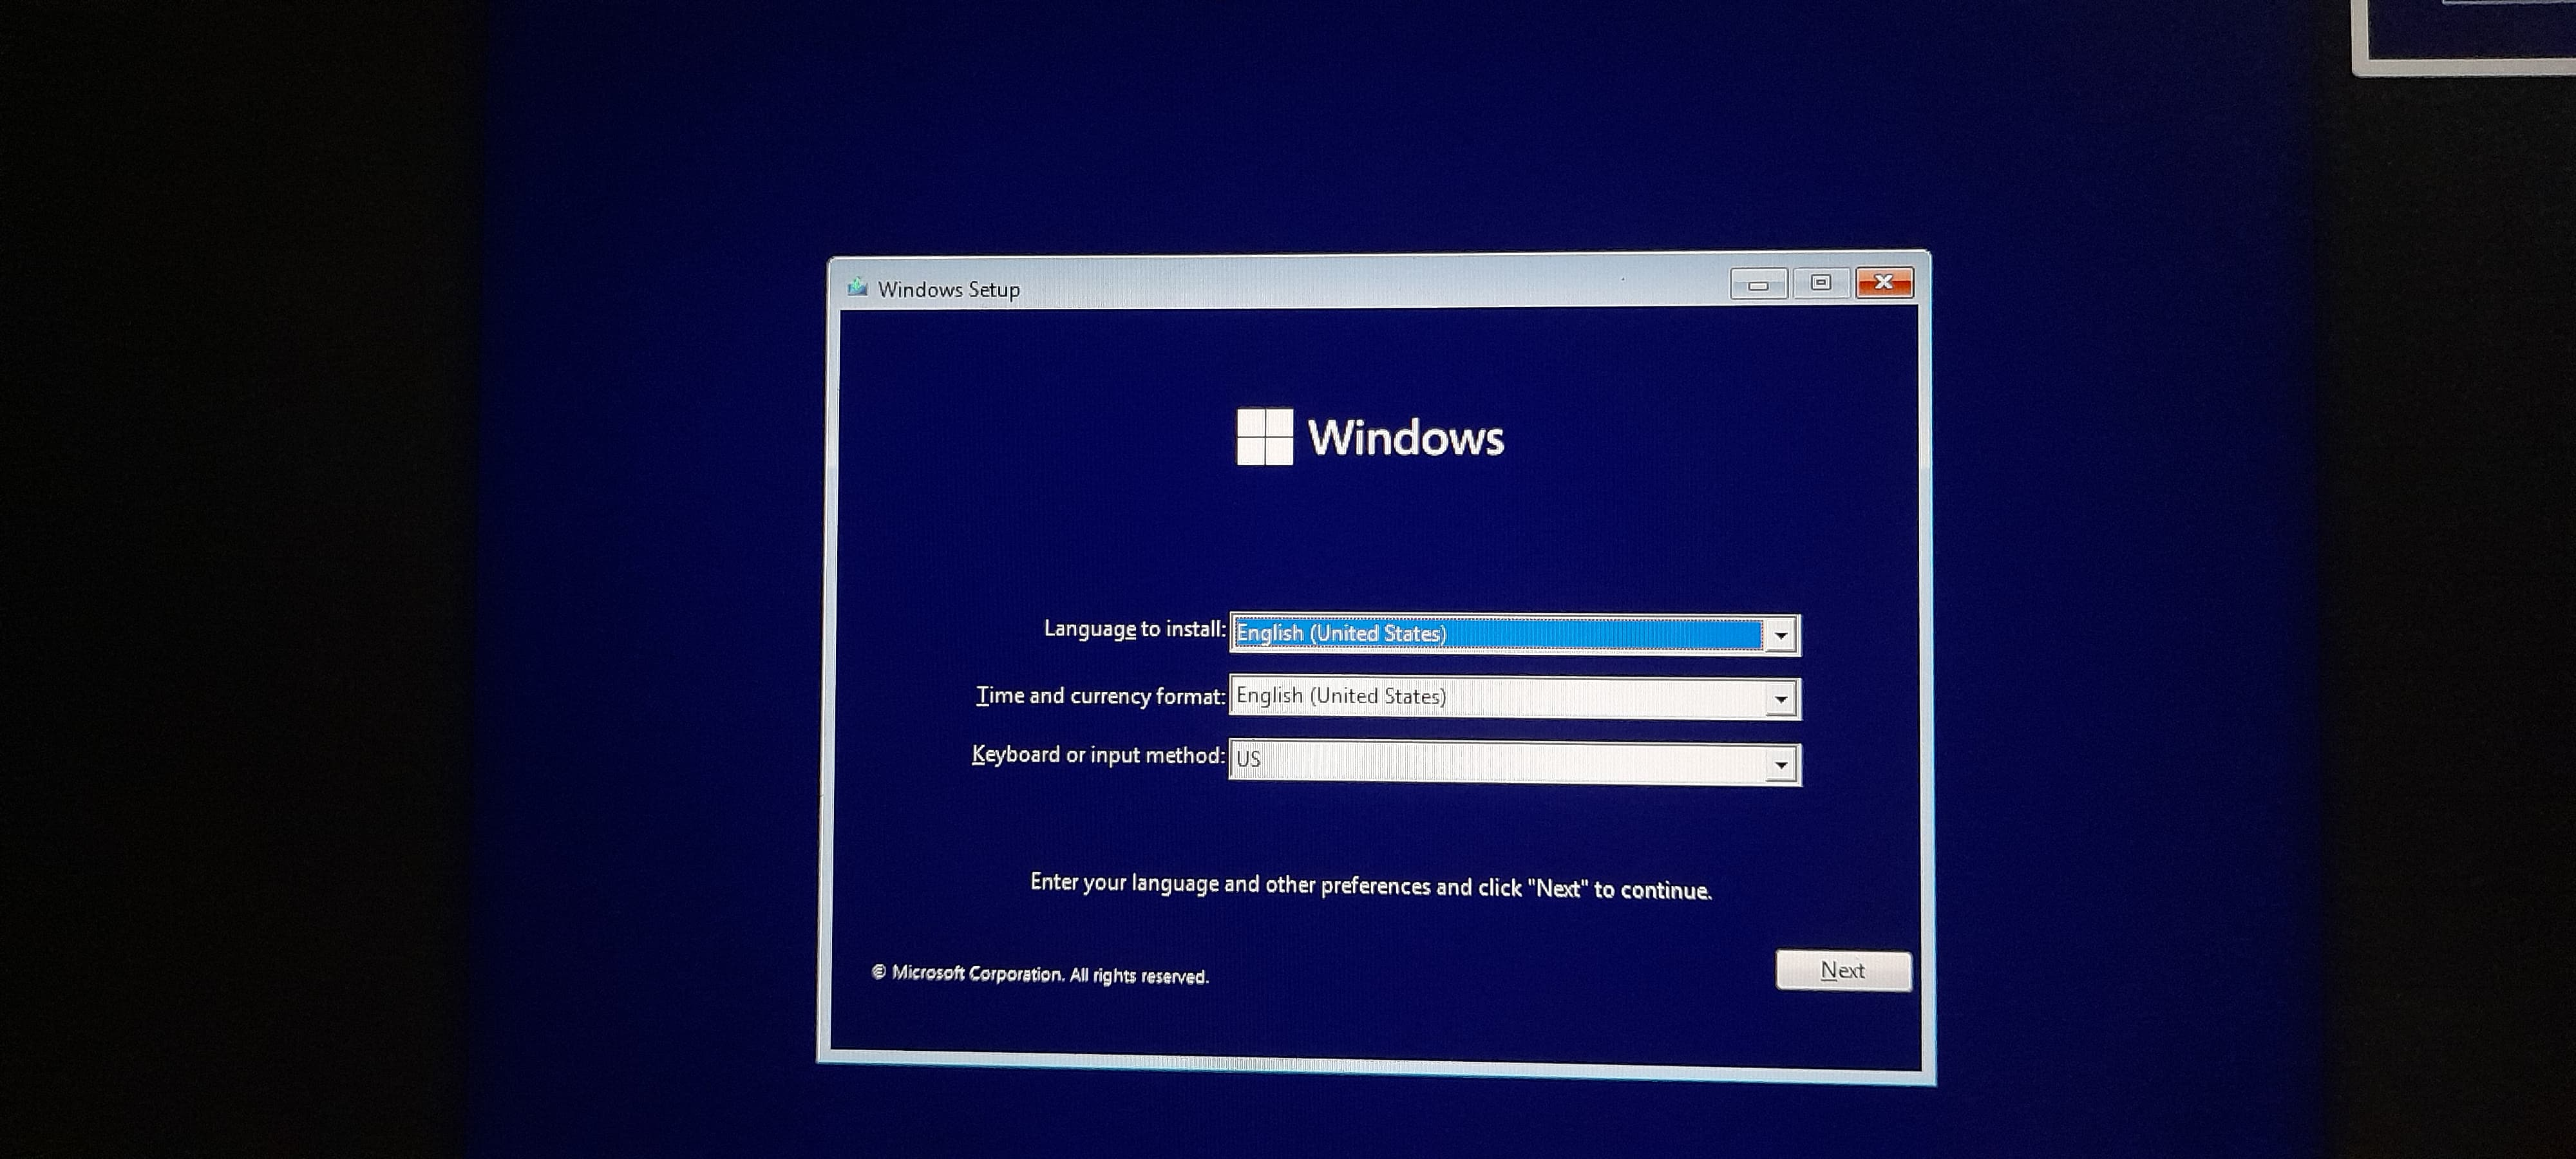
\includegraphics[width=0.8\textwidth]{9.jpeg} % Placeholder for UEFI & ISO screenshot
    \captionof{figure}{Installation of Windows}
\end{center}
\begin{center}
    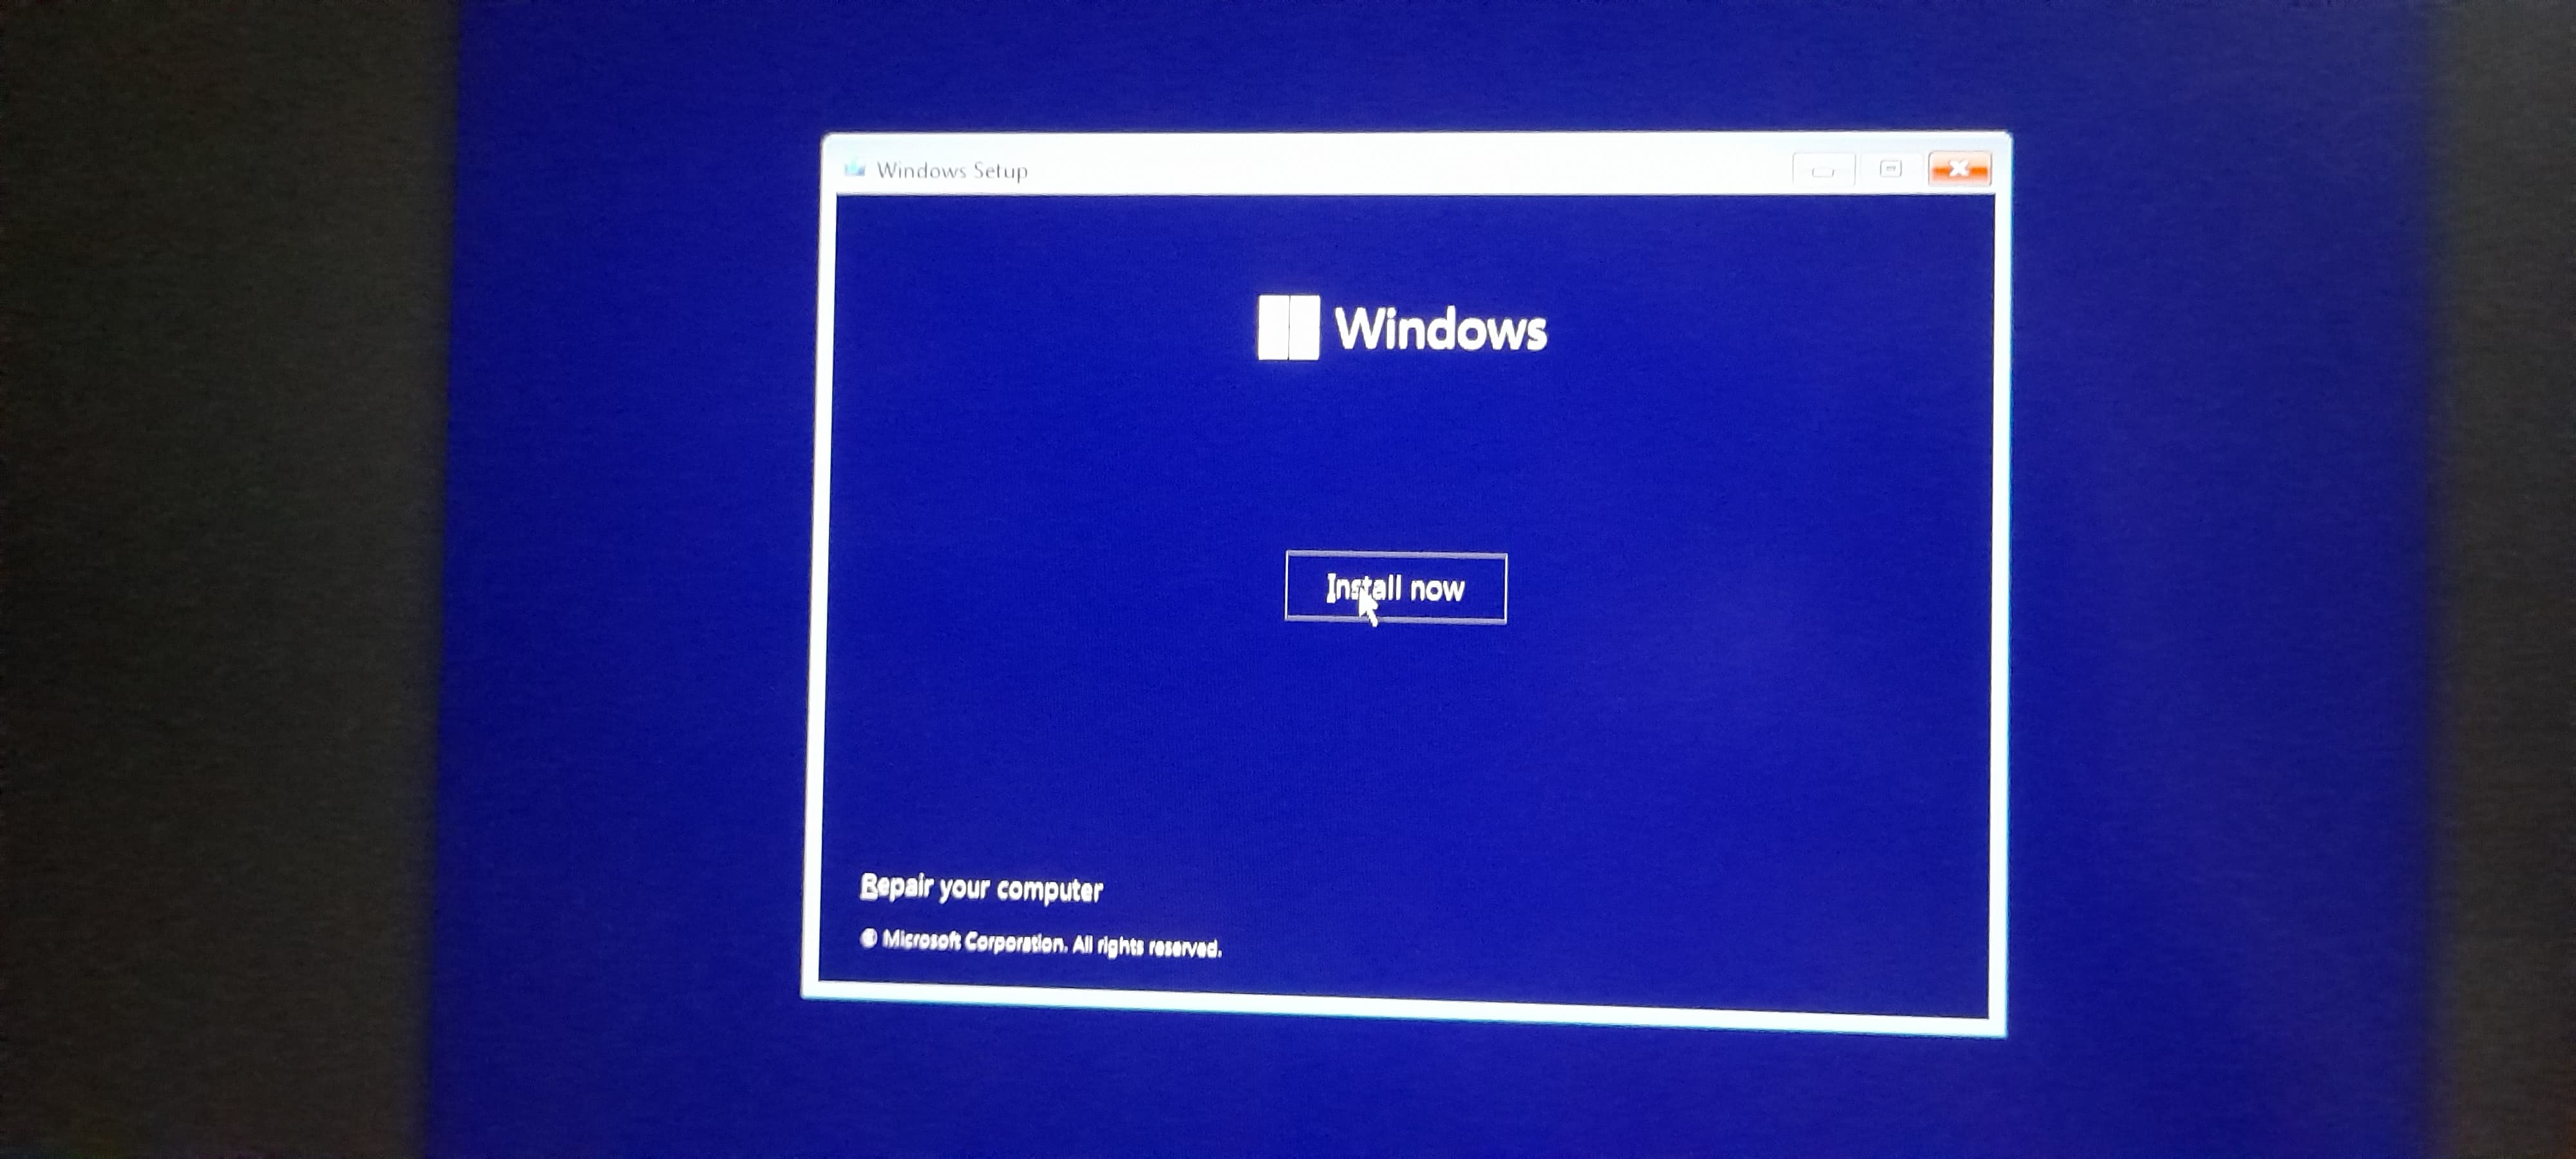
\includegraphics[width=0.8\textwidth]{10.jpeg} % Placeholder for UEFI & ISO screenshot
    \captionof{figure}{Installation of Windows}
\end{center}
\begin{center}
    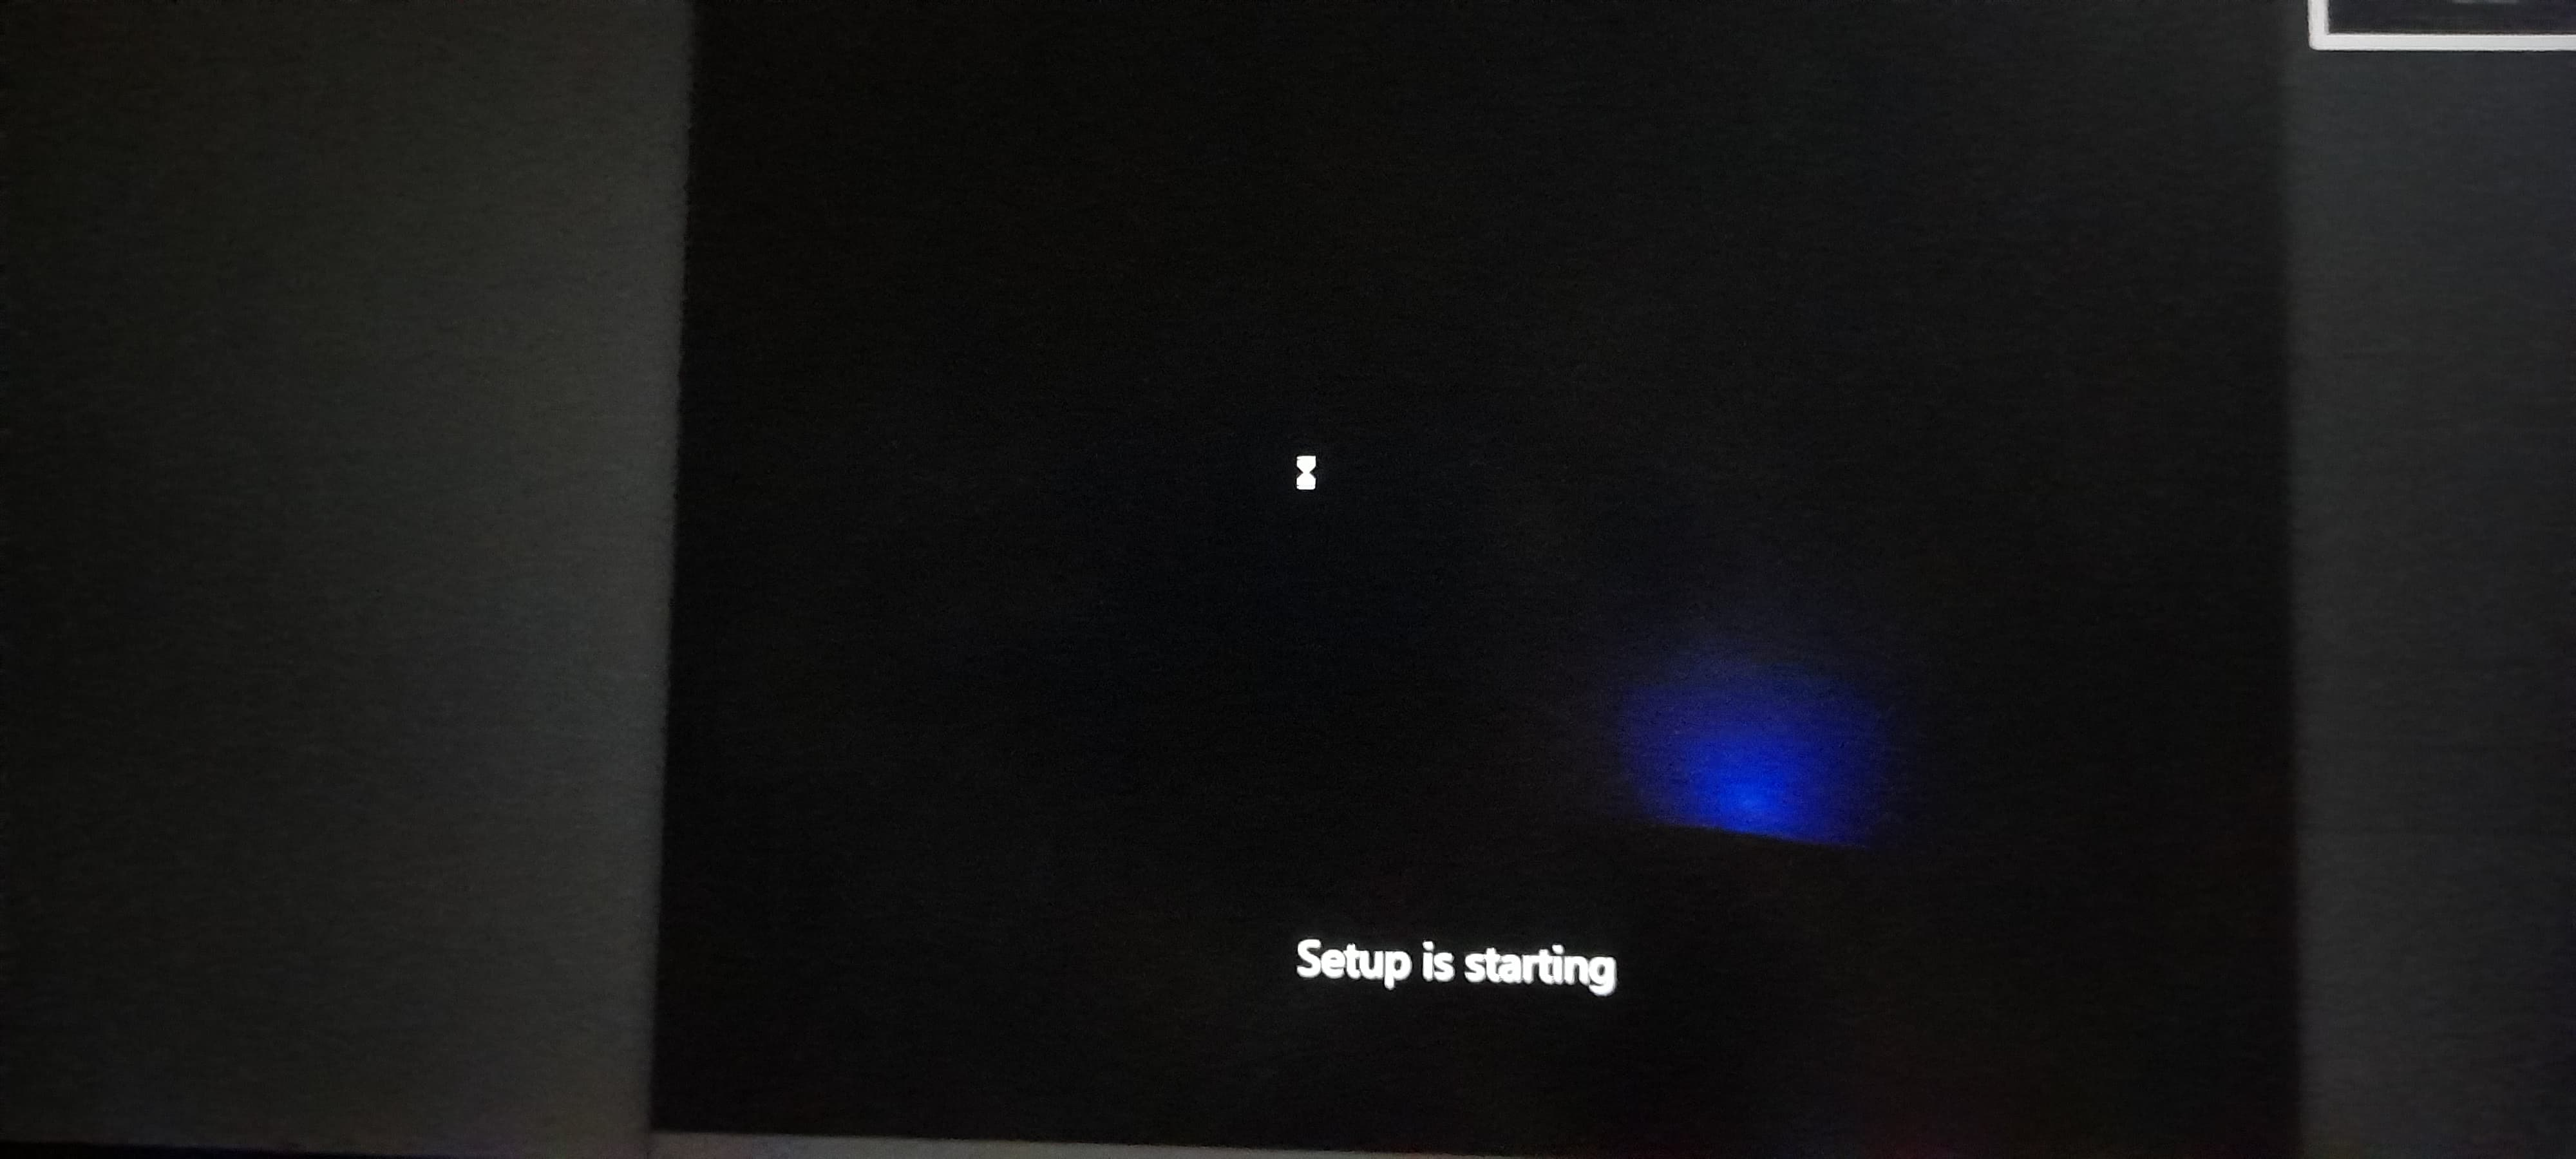
\includegraphics[width=0.8\textwidth]{11.jpeg} % Placeholder for UEFI & ISO screenshot
    \captionof{figure}{Installation of Windows}
\end{center}
\begin{center}
    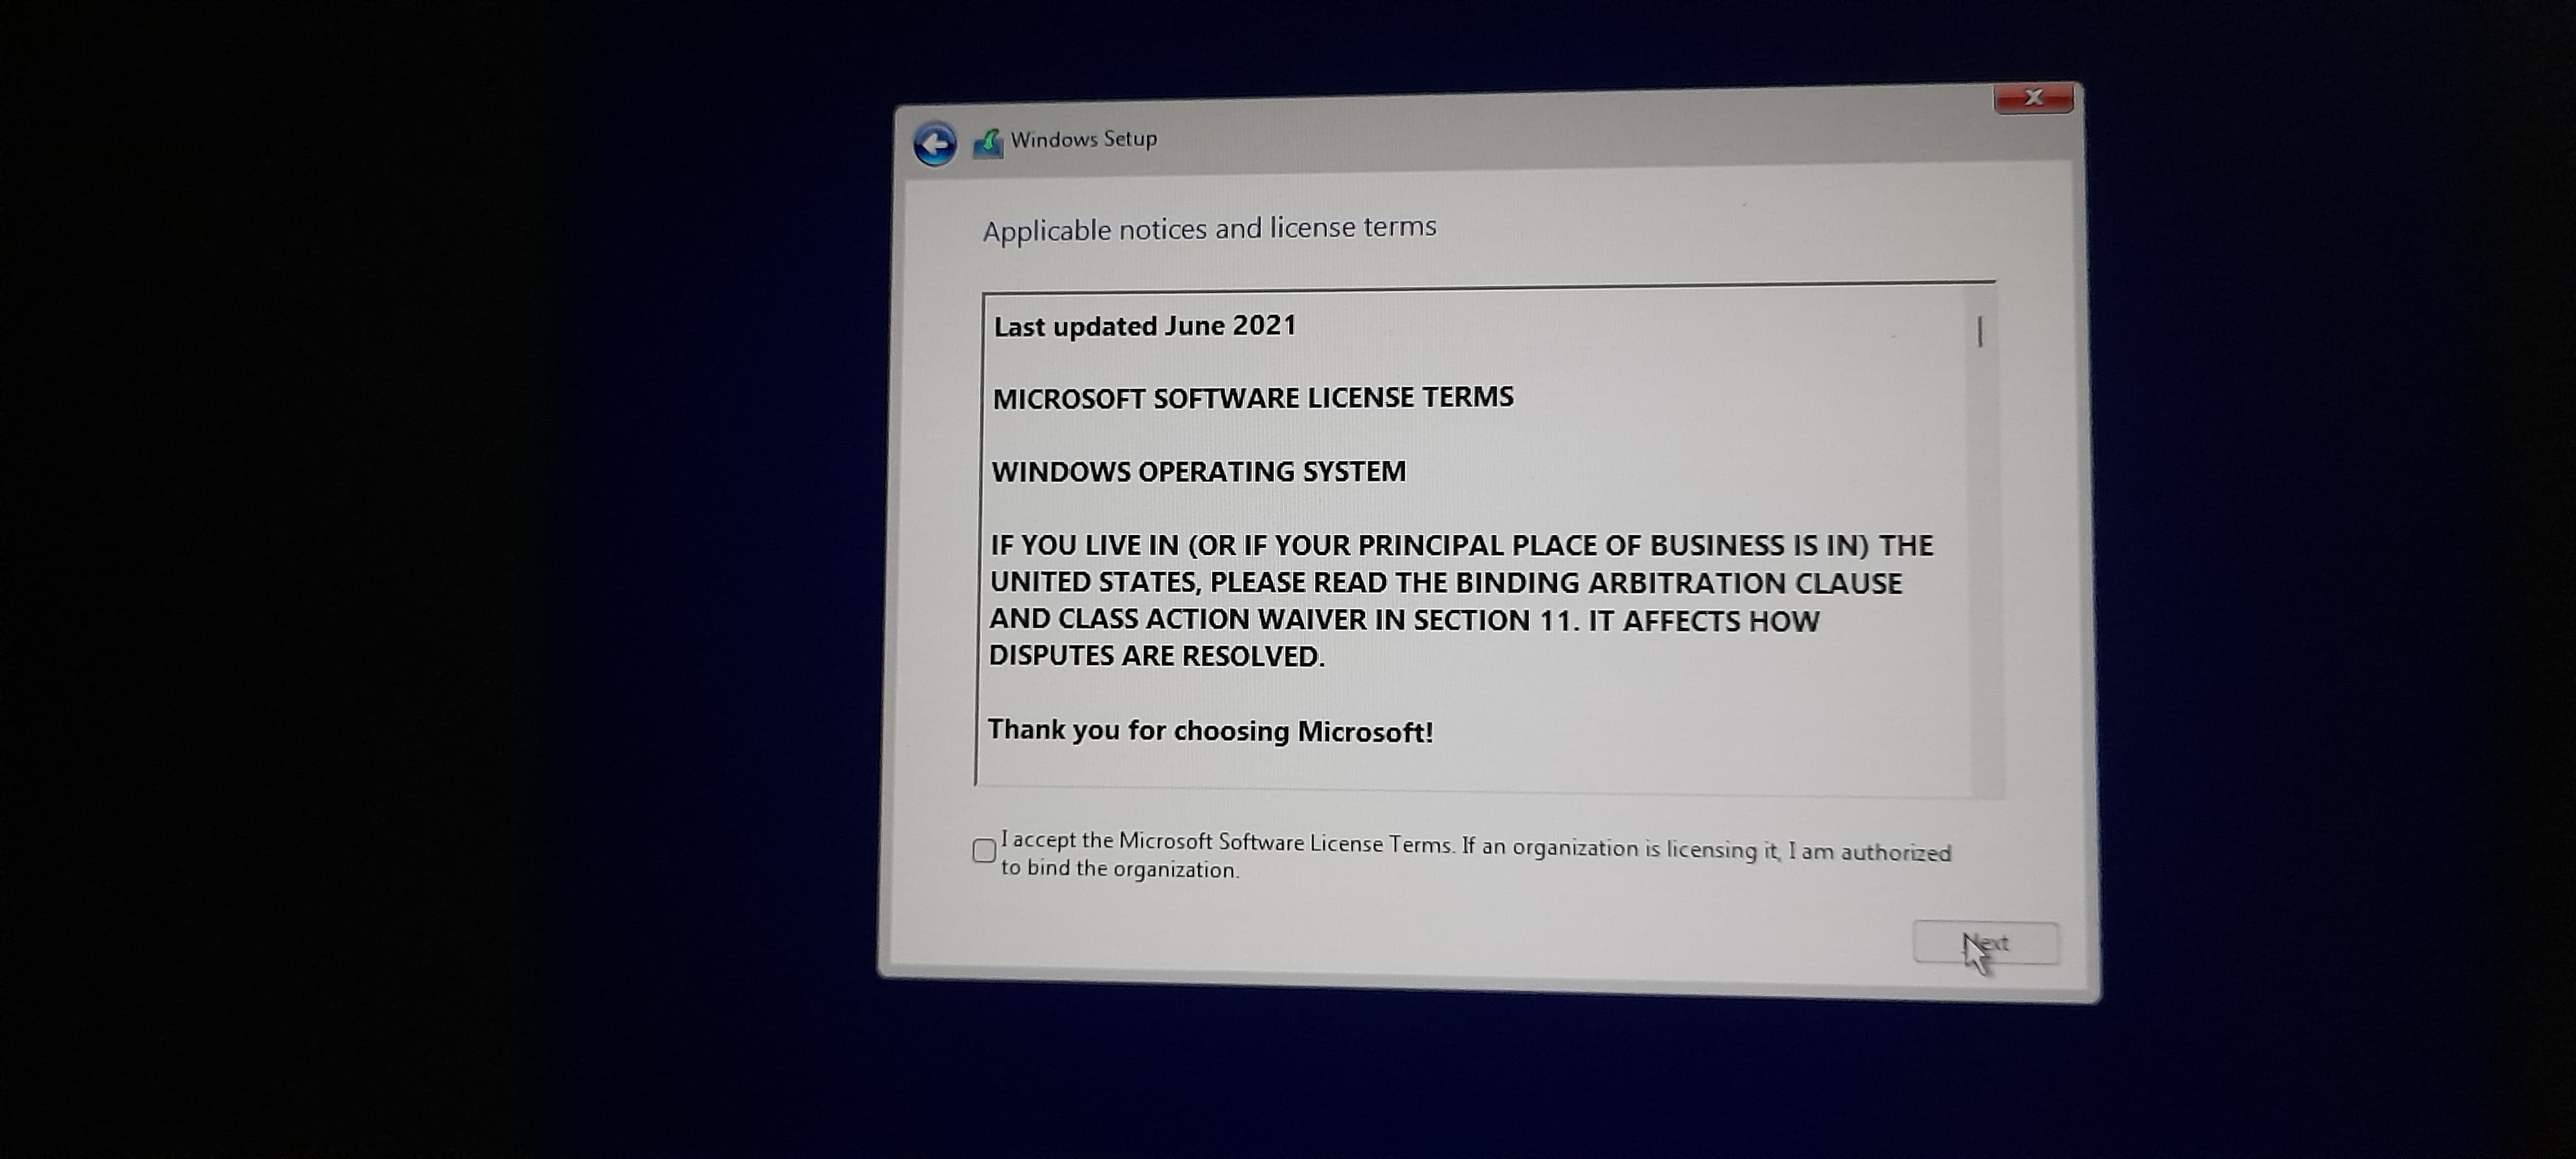
\includegraphics[width=0.8\textwidth]{12.jpeg} % Placeholder for UEFI & ISO screenshot
    \captionof{figure}{Installation of Windows}
\end{center}

\subsection{Partition Setup}
During installation, create the following partitions:
\begin{itemize}
    \item \textbf{62GB} for Windows 11
    \item \textbf{33GB} for Arch Linux
    \item \textbf{24GB} for Ubuntu
\end{itemize}

\begin{center}
    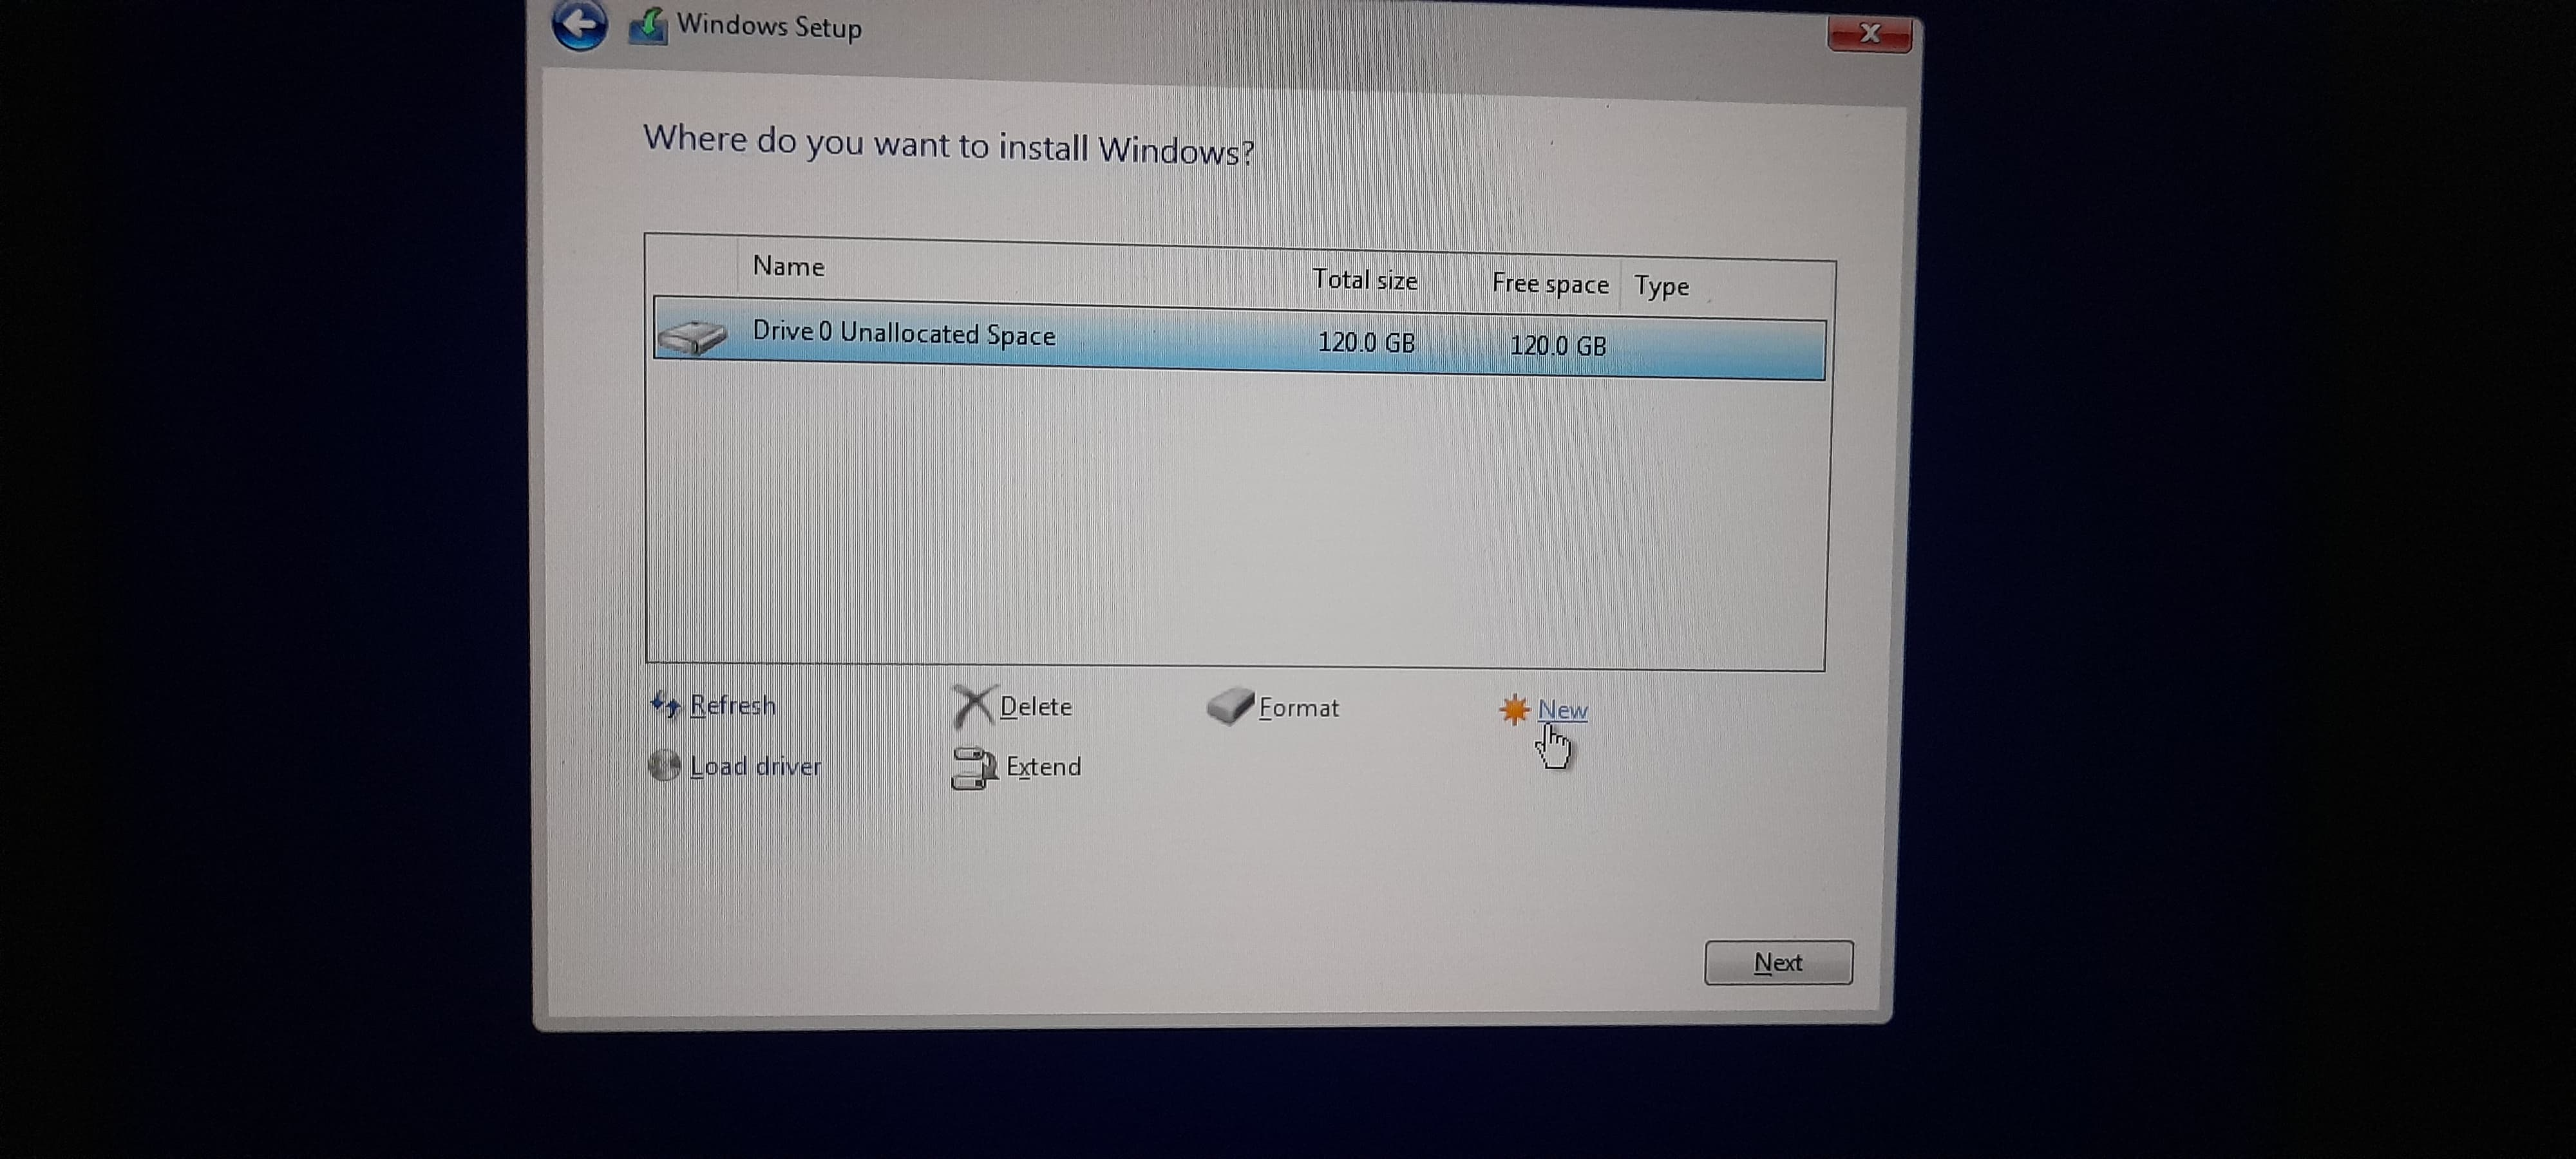
\includegraphics[width=0.8\textwidth]{13.jpeg} % Placeholder for partition creation screenshot
    \captionof{figure}{Partition Setup for Windows, Arch, and Ubuntu}
\end{center}
\begin{center}
    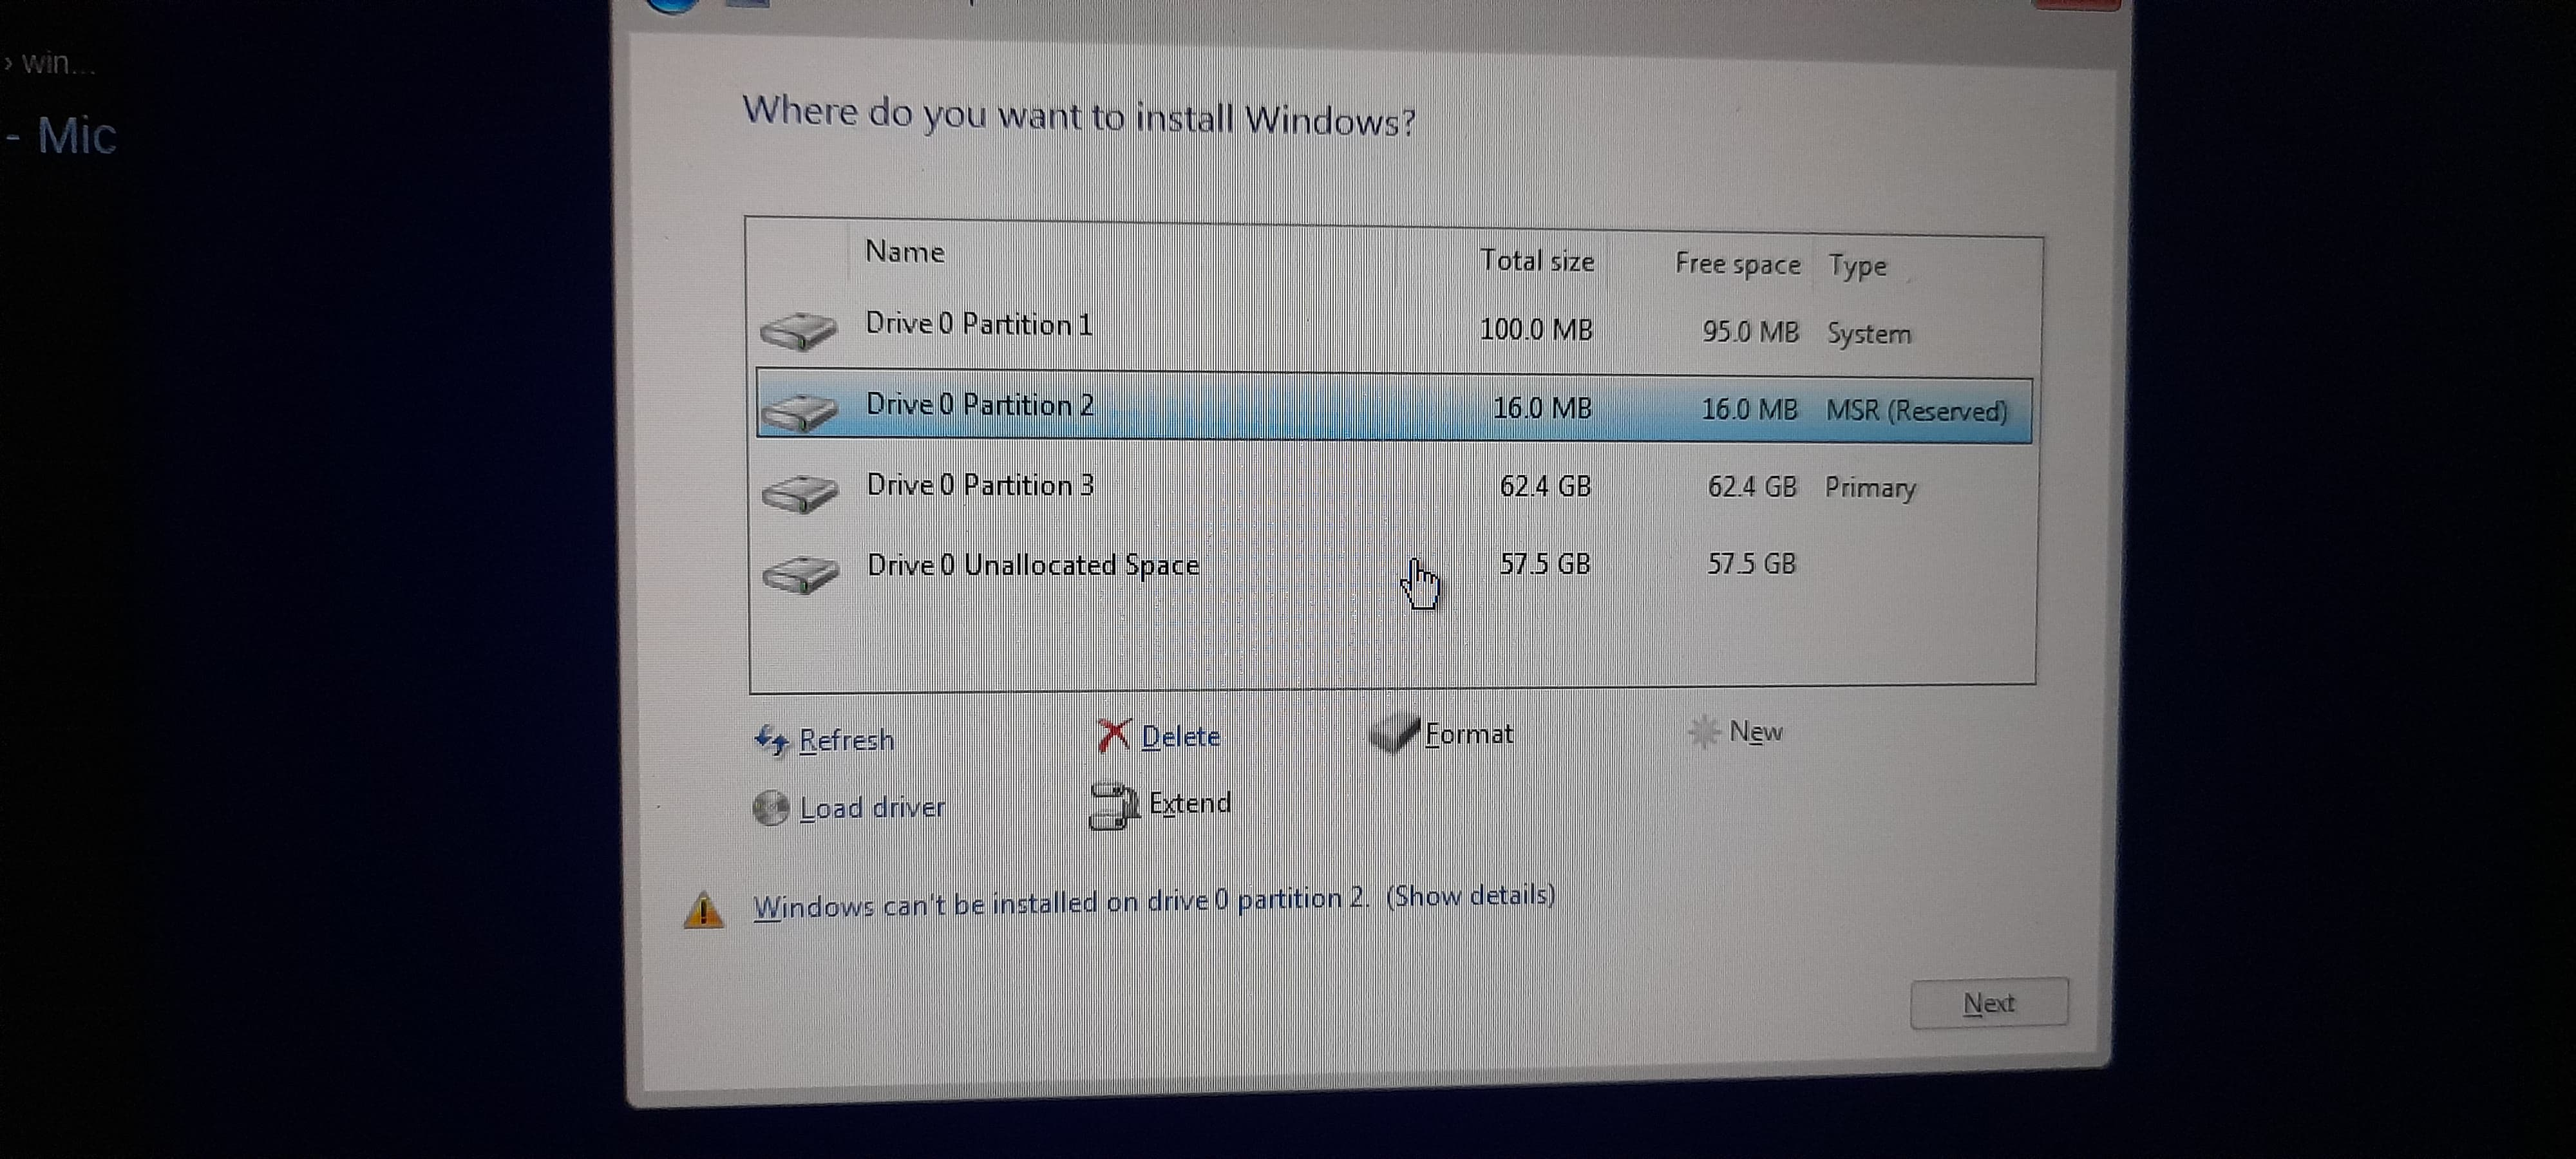
\includegraphics[width=0.8\textwidth]{14.jpeg} % Placeholder for partition creation screenshot
    \captionof{figure}{Partition Setup for Windows, Arch, and Ubuntu}
\end{center}
\begin{center}
    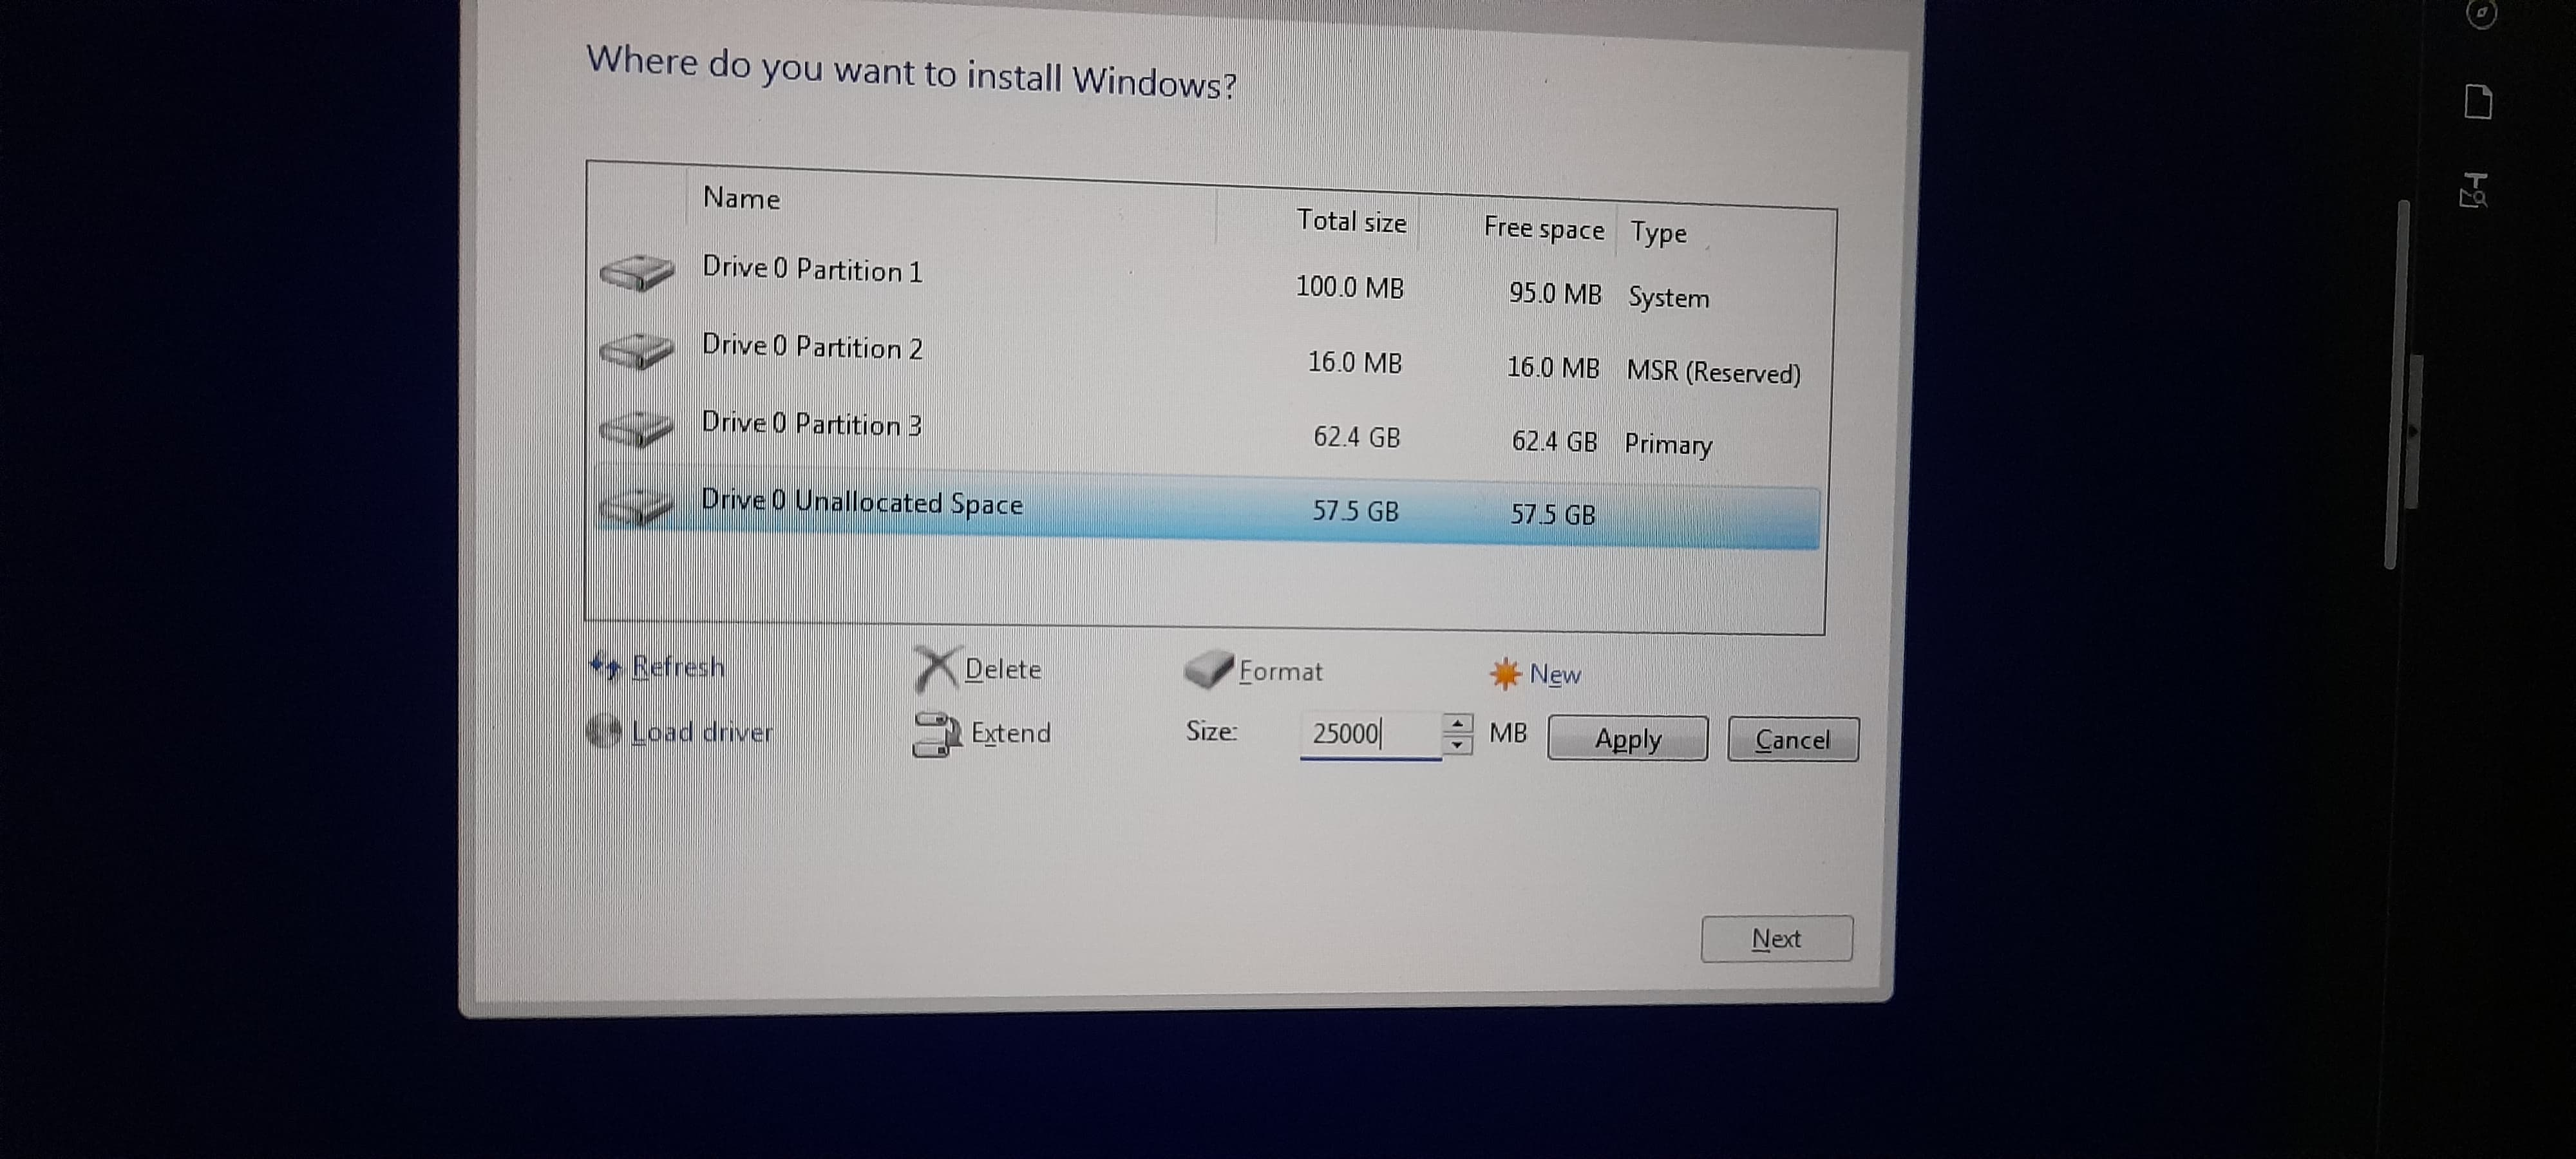
\includegraphics[width=0.8\textwidth]{15.jpeg} % Placeholder for partition creation screenshot
    \captionof{figure}{Partition Setup for Windows, Arch, and Ubuntu}
\end{center}
\begin{center}
    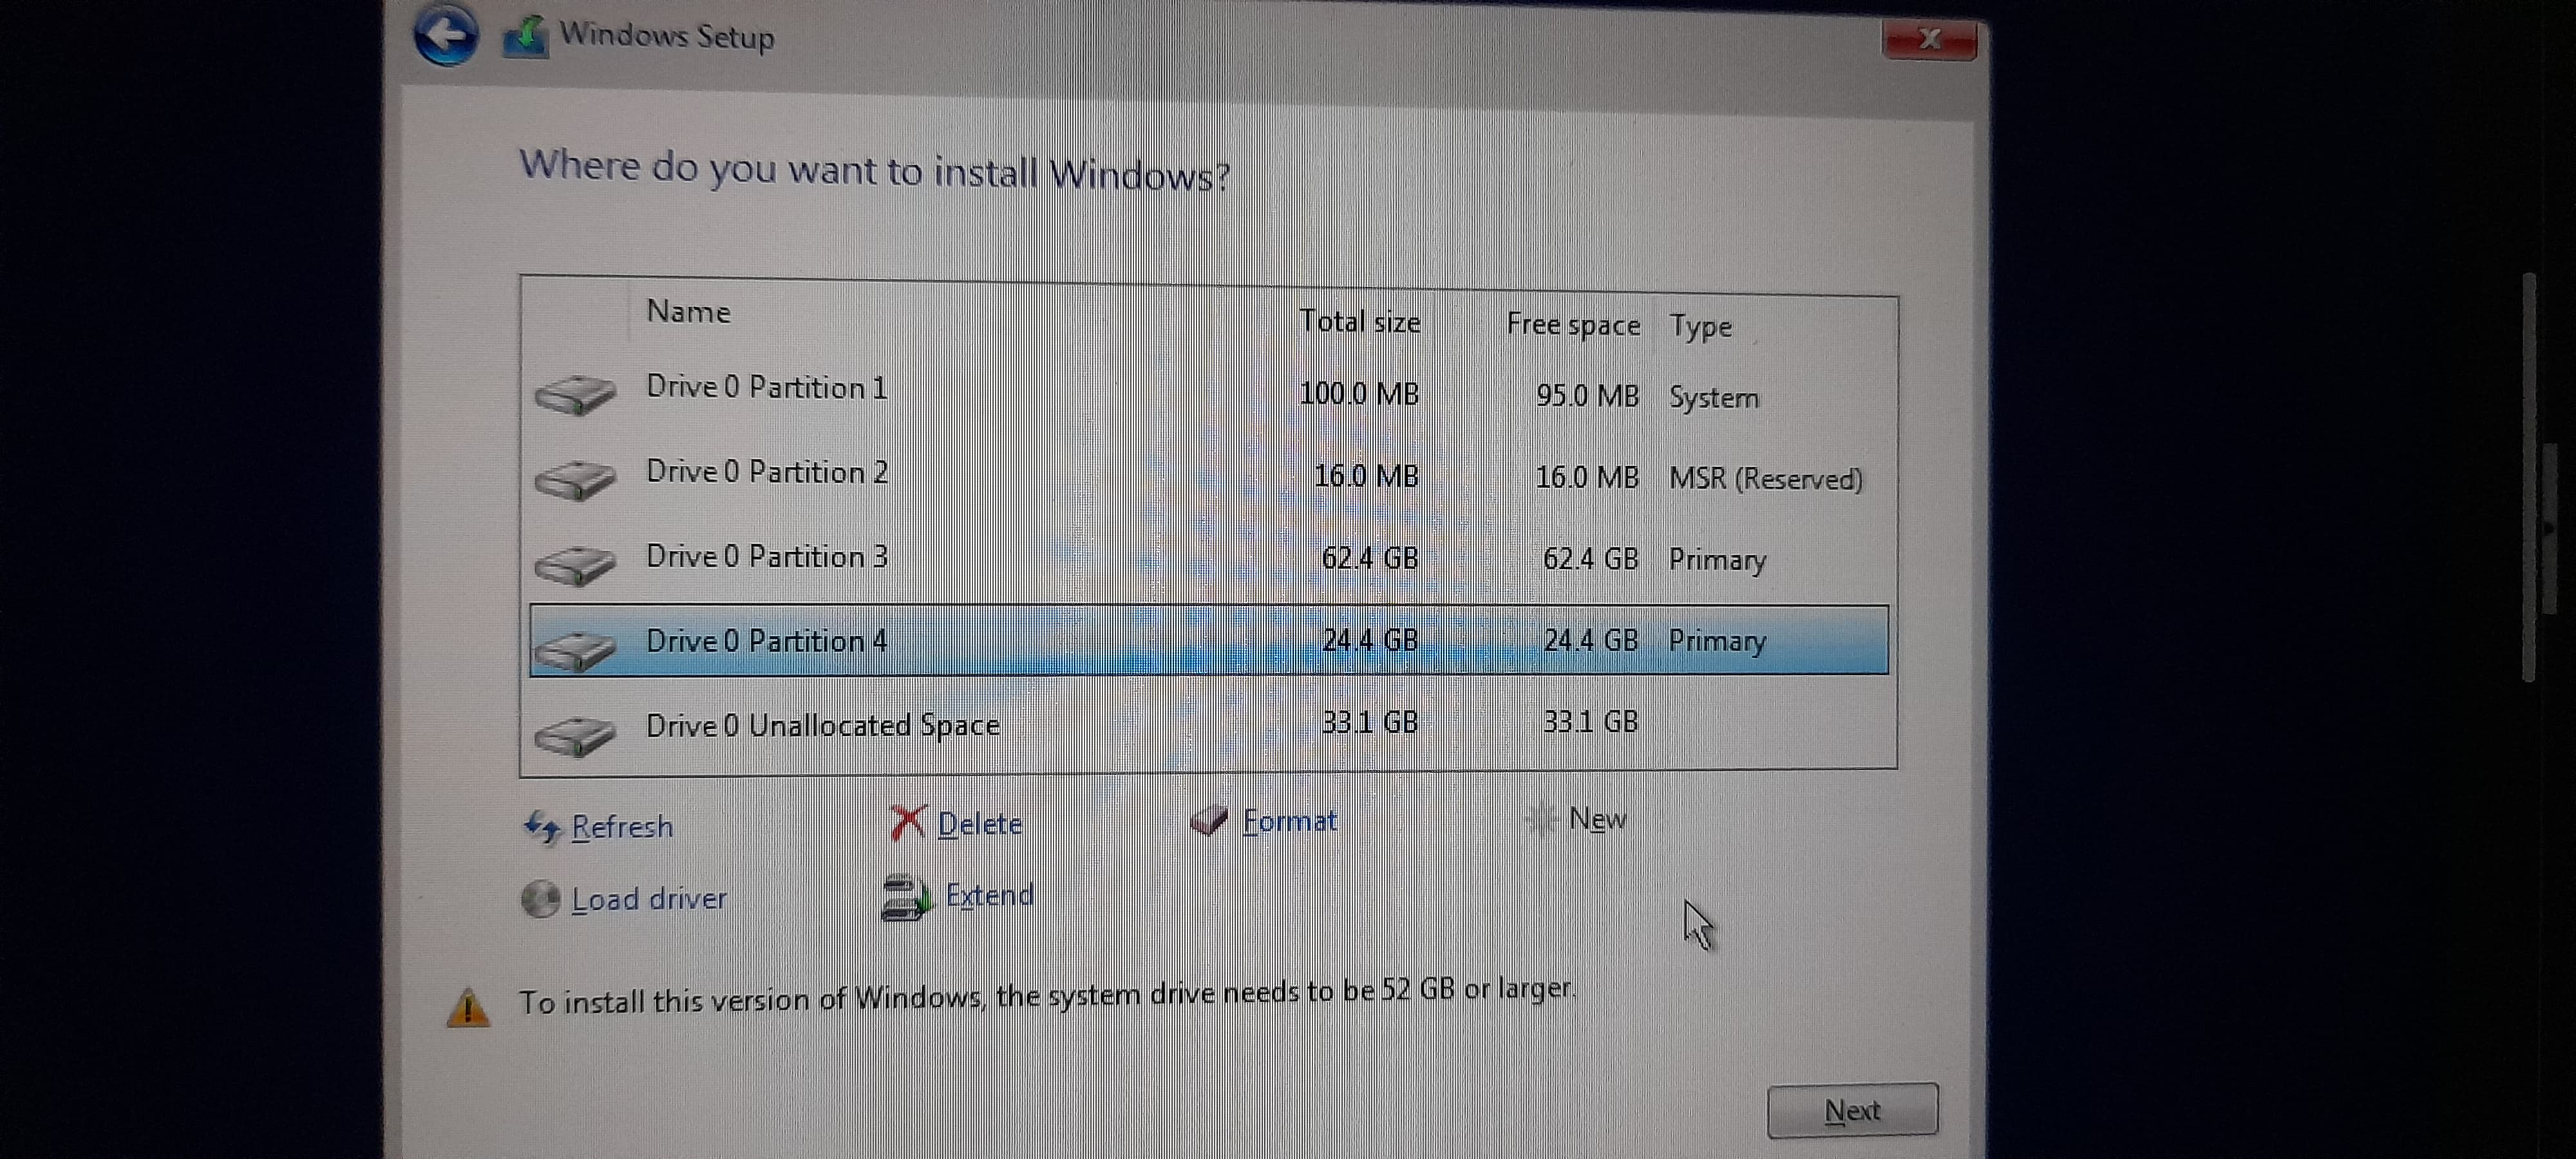
\includegraphics[width=0.8\textwidth]{16.jpeg} % Placeholder for partition creation screenshot
    \captionof{figure}{Partition Setup for Windows, Arch, and Ubuntu}
\end{center}
\begin{center}
    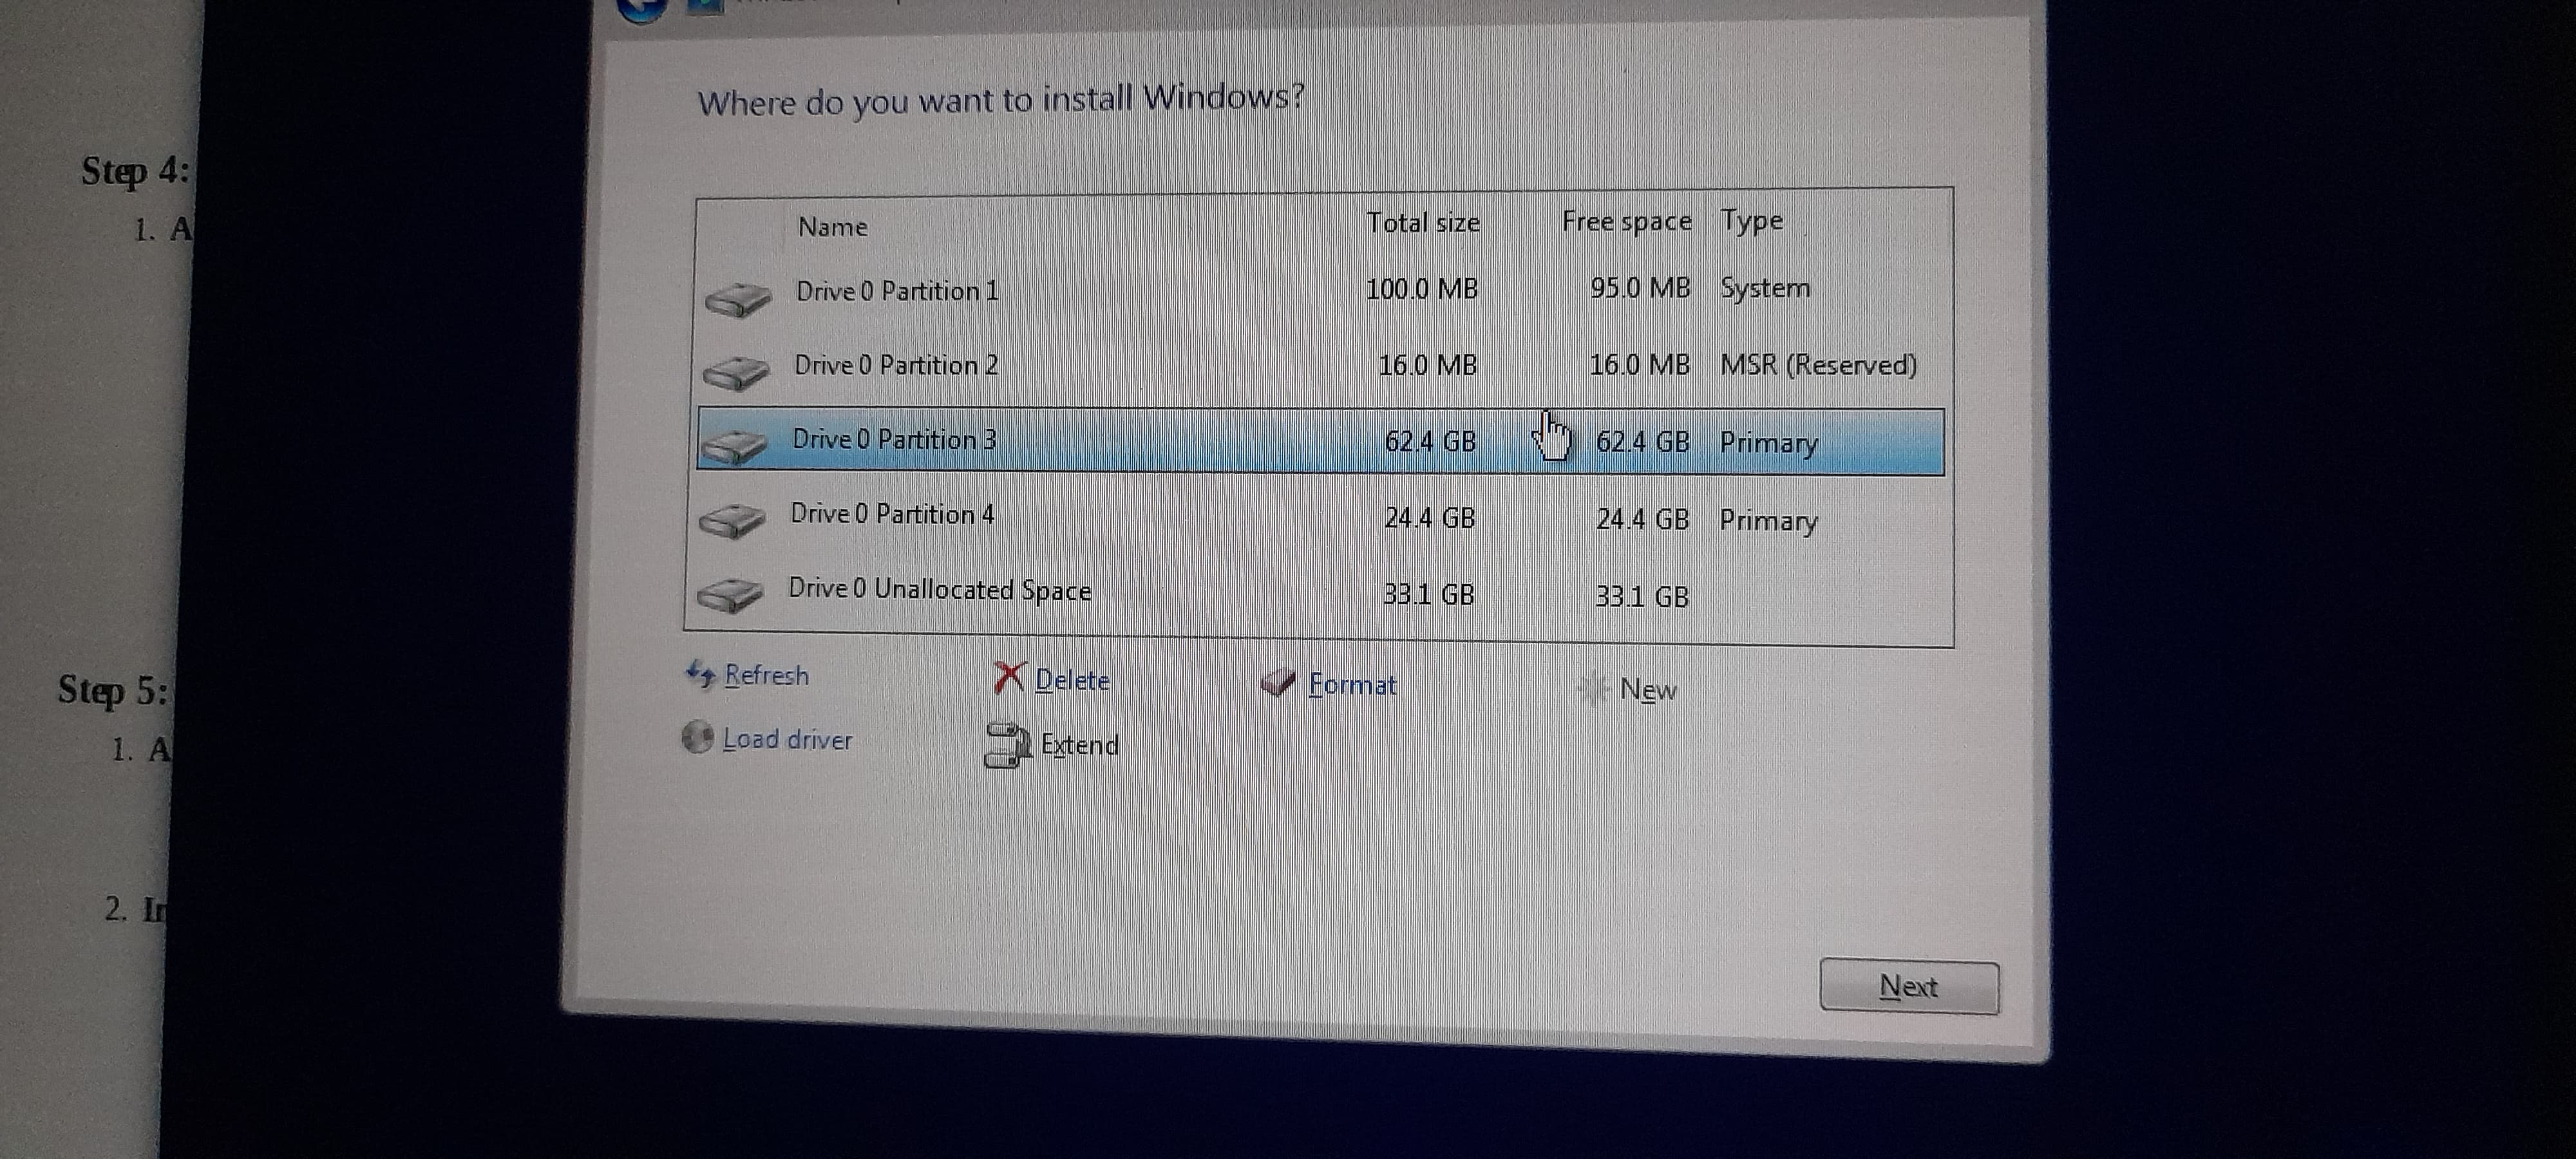
\includegraphics[width=0.8\textwidth]{17.jpeg} % Placeholder for partition creation screenshot
    \captionof{figure}{Partition Setup for Windows, Arch, and Ubuntu}
\end{center}

\subsection{Naming the Device and Disk Management}
Once installation completes, name your device and verify the partitions using the Disk Management tool.

\begin{center}
    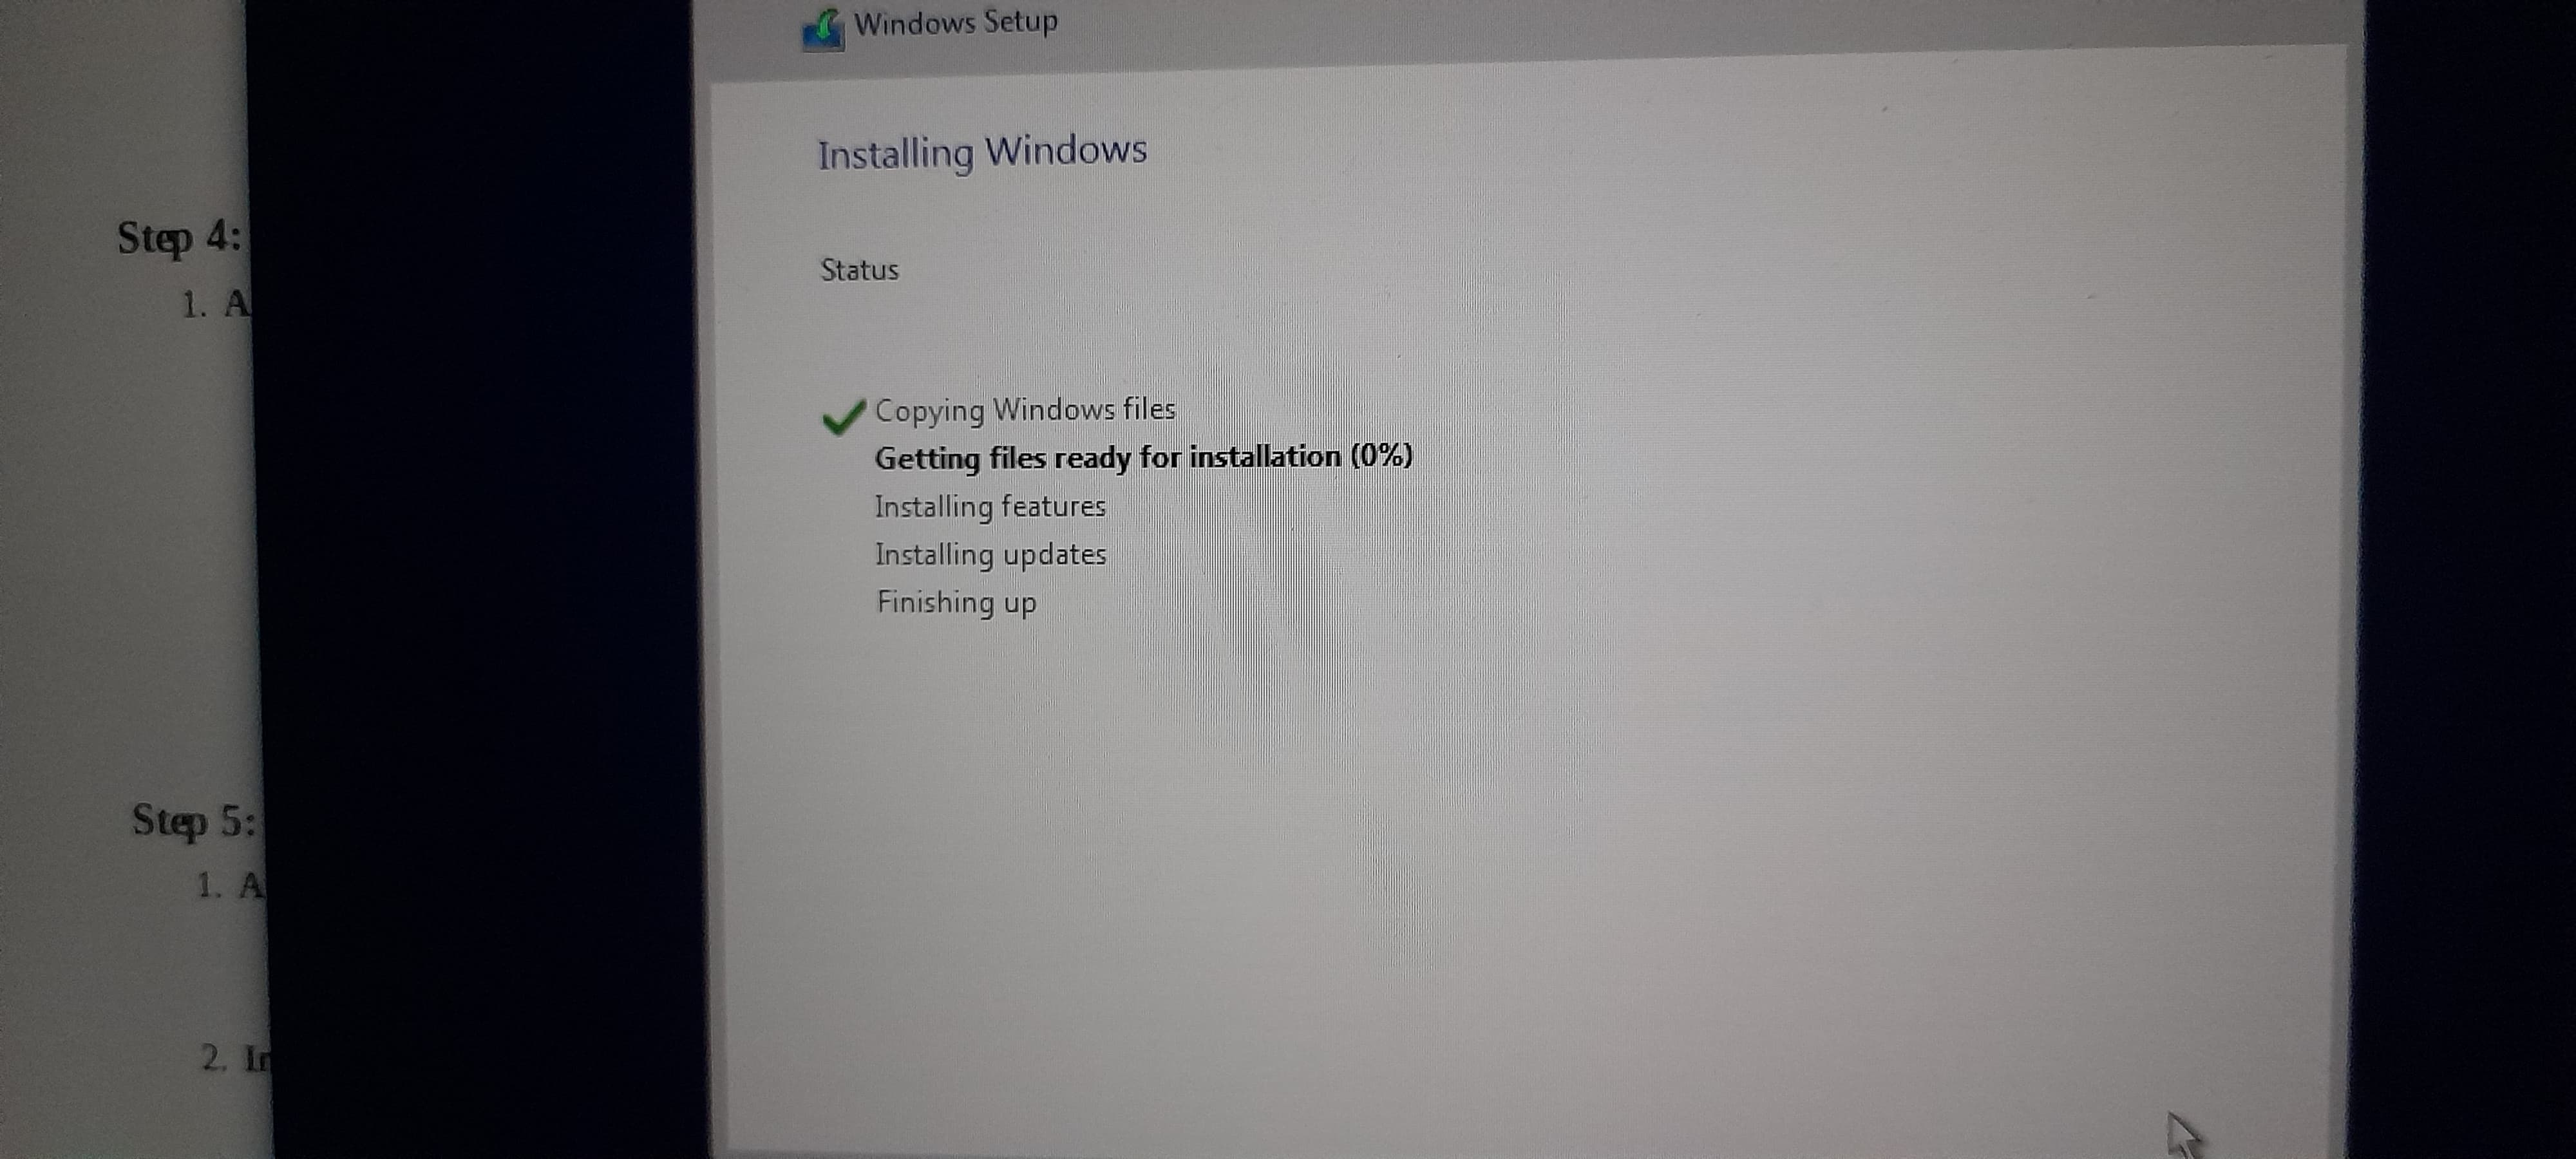
\includegraphics[width=0.8\textwidth]{18.jpeg} % Placeholder for device naming screenshot
    \captionof{figure}{Setup}
\end{center}
\begin{center}
    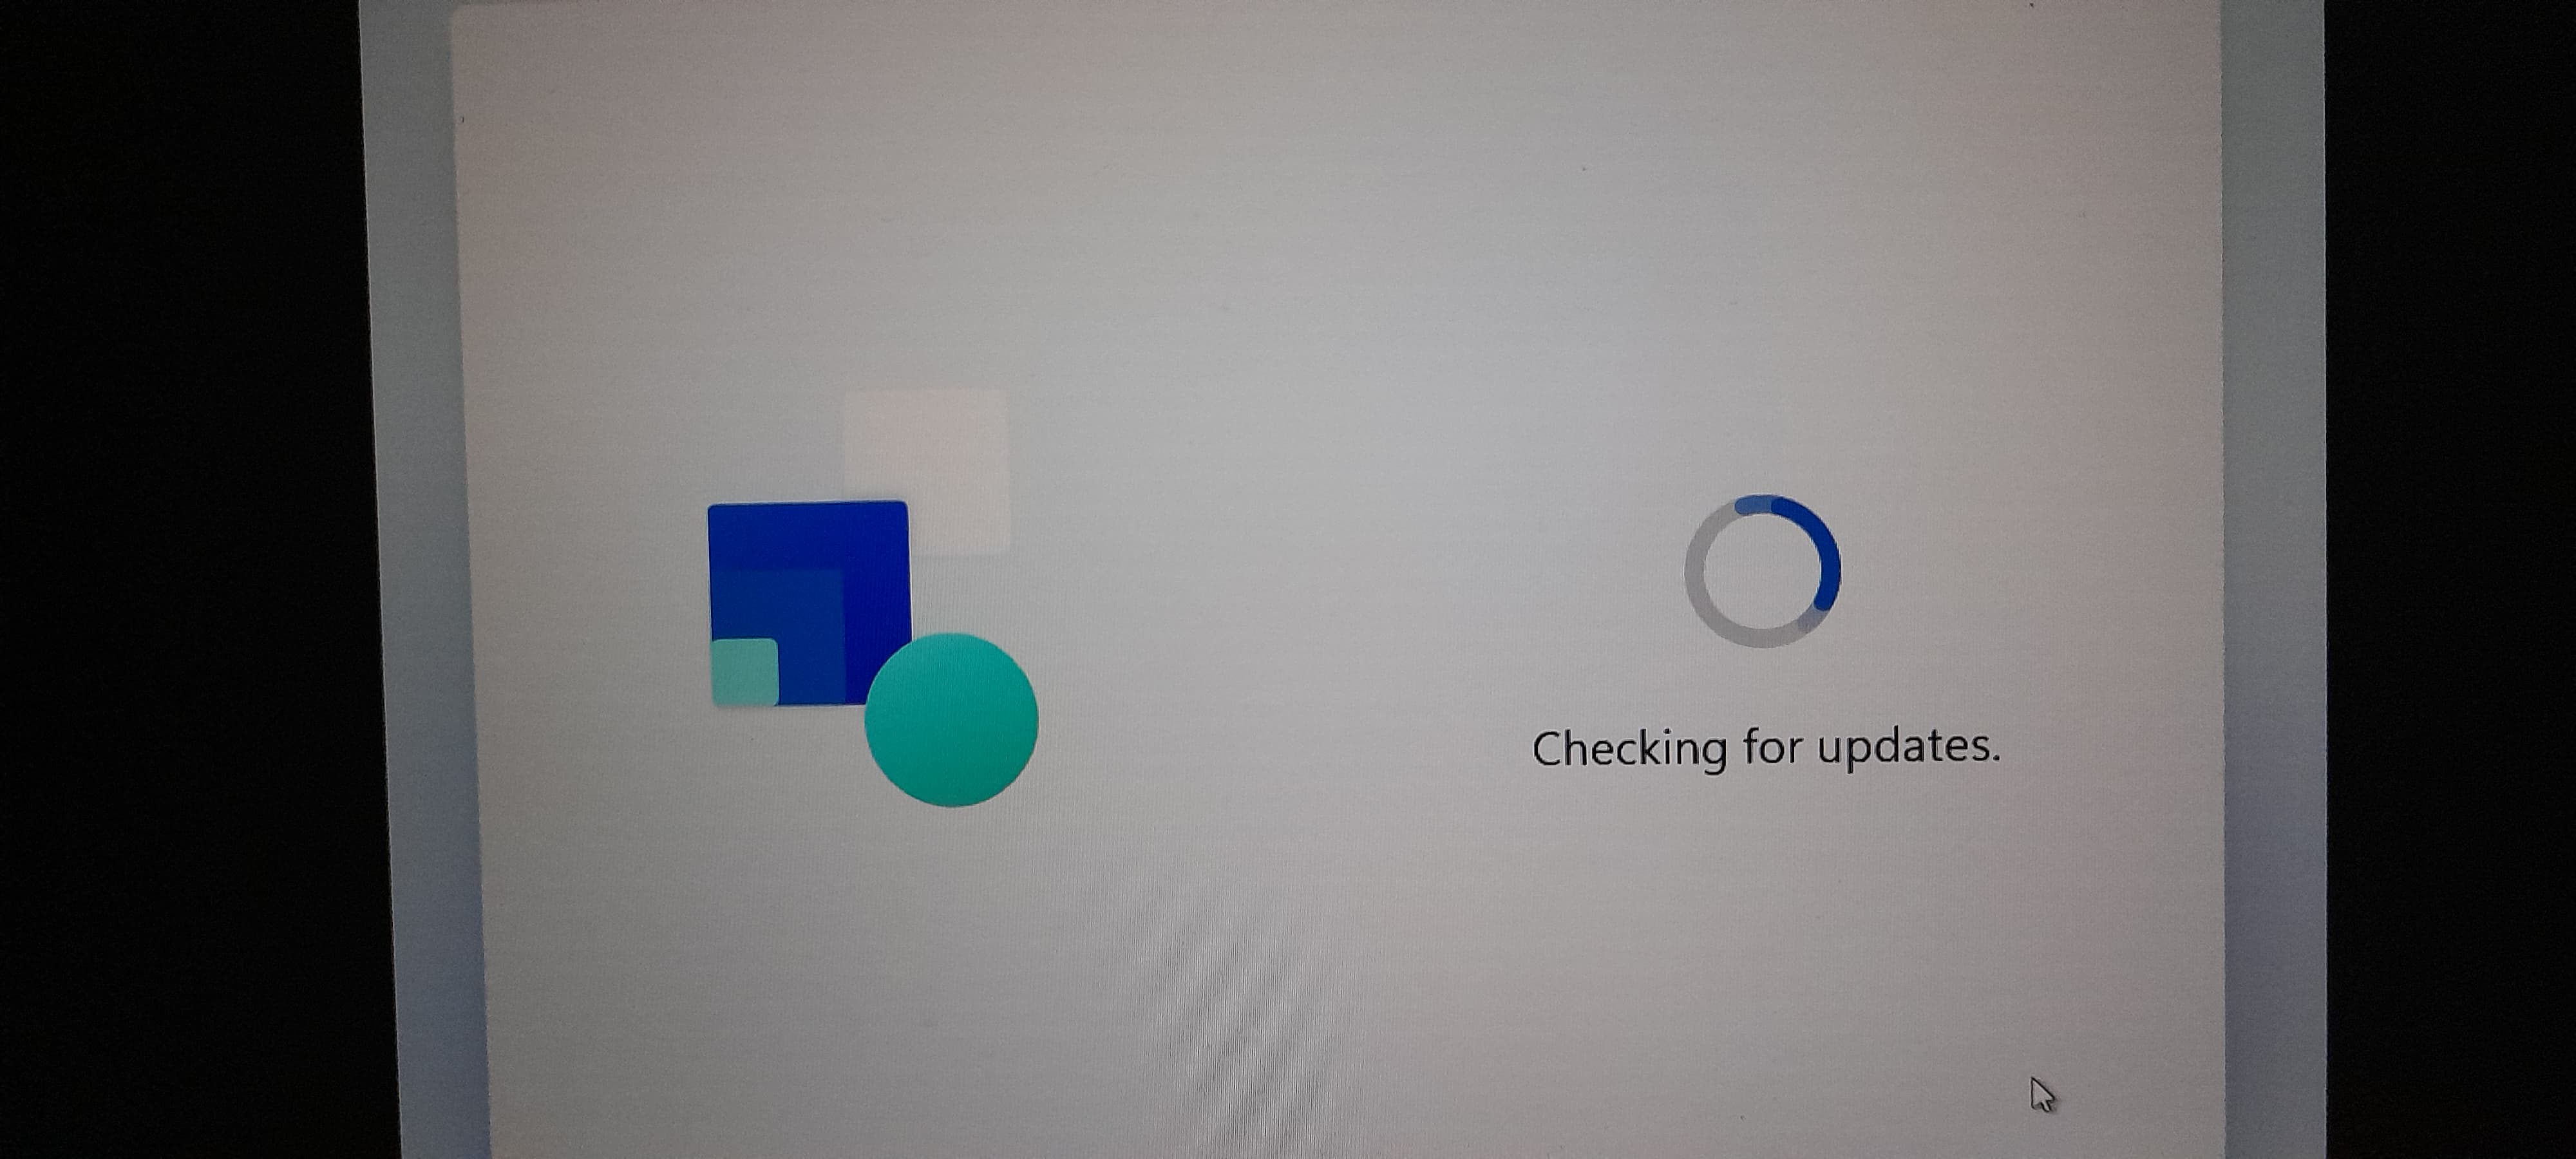
\includegraphics[width=0.8\textwidth]{19.jpeg} % Placeholder for device naming screenshot
    \captionof{figure}{Setup}
\end{center}
\begin{center}
    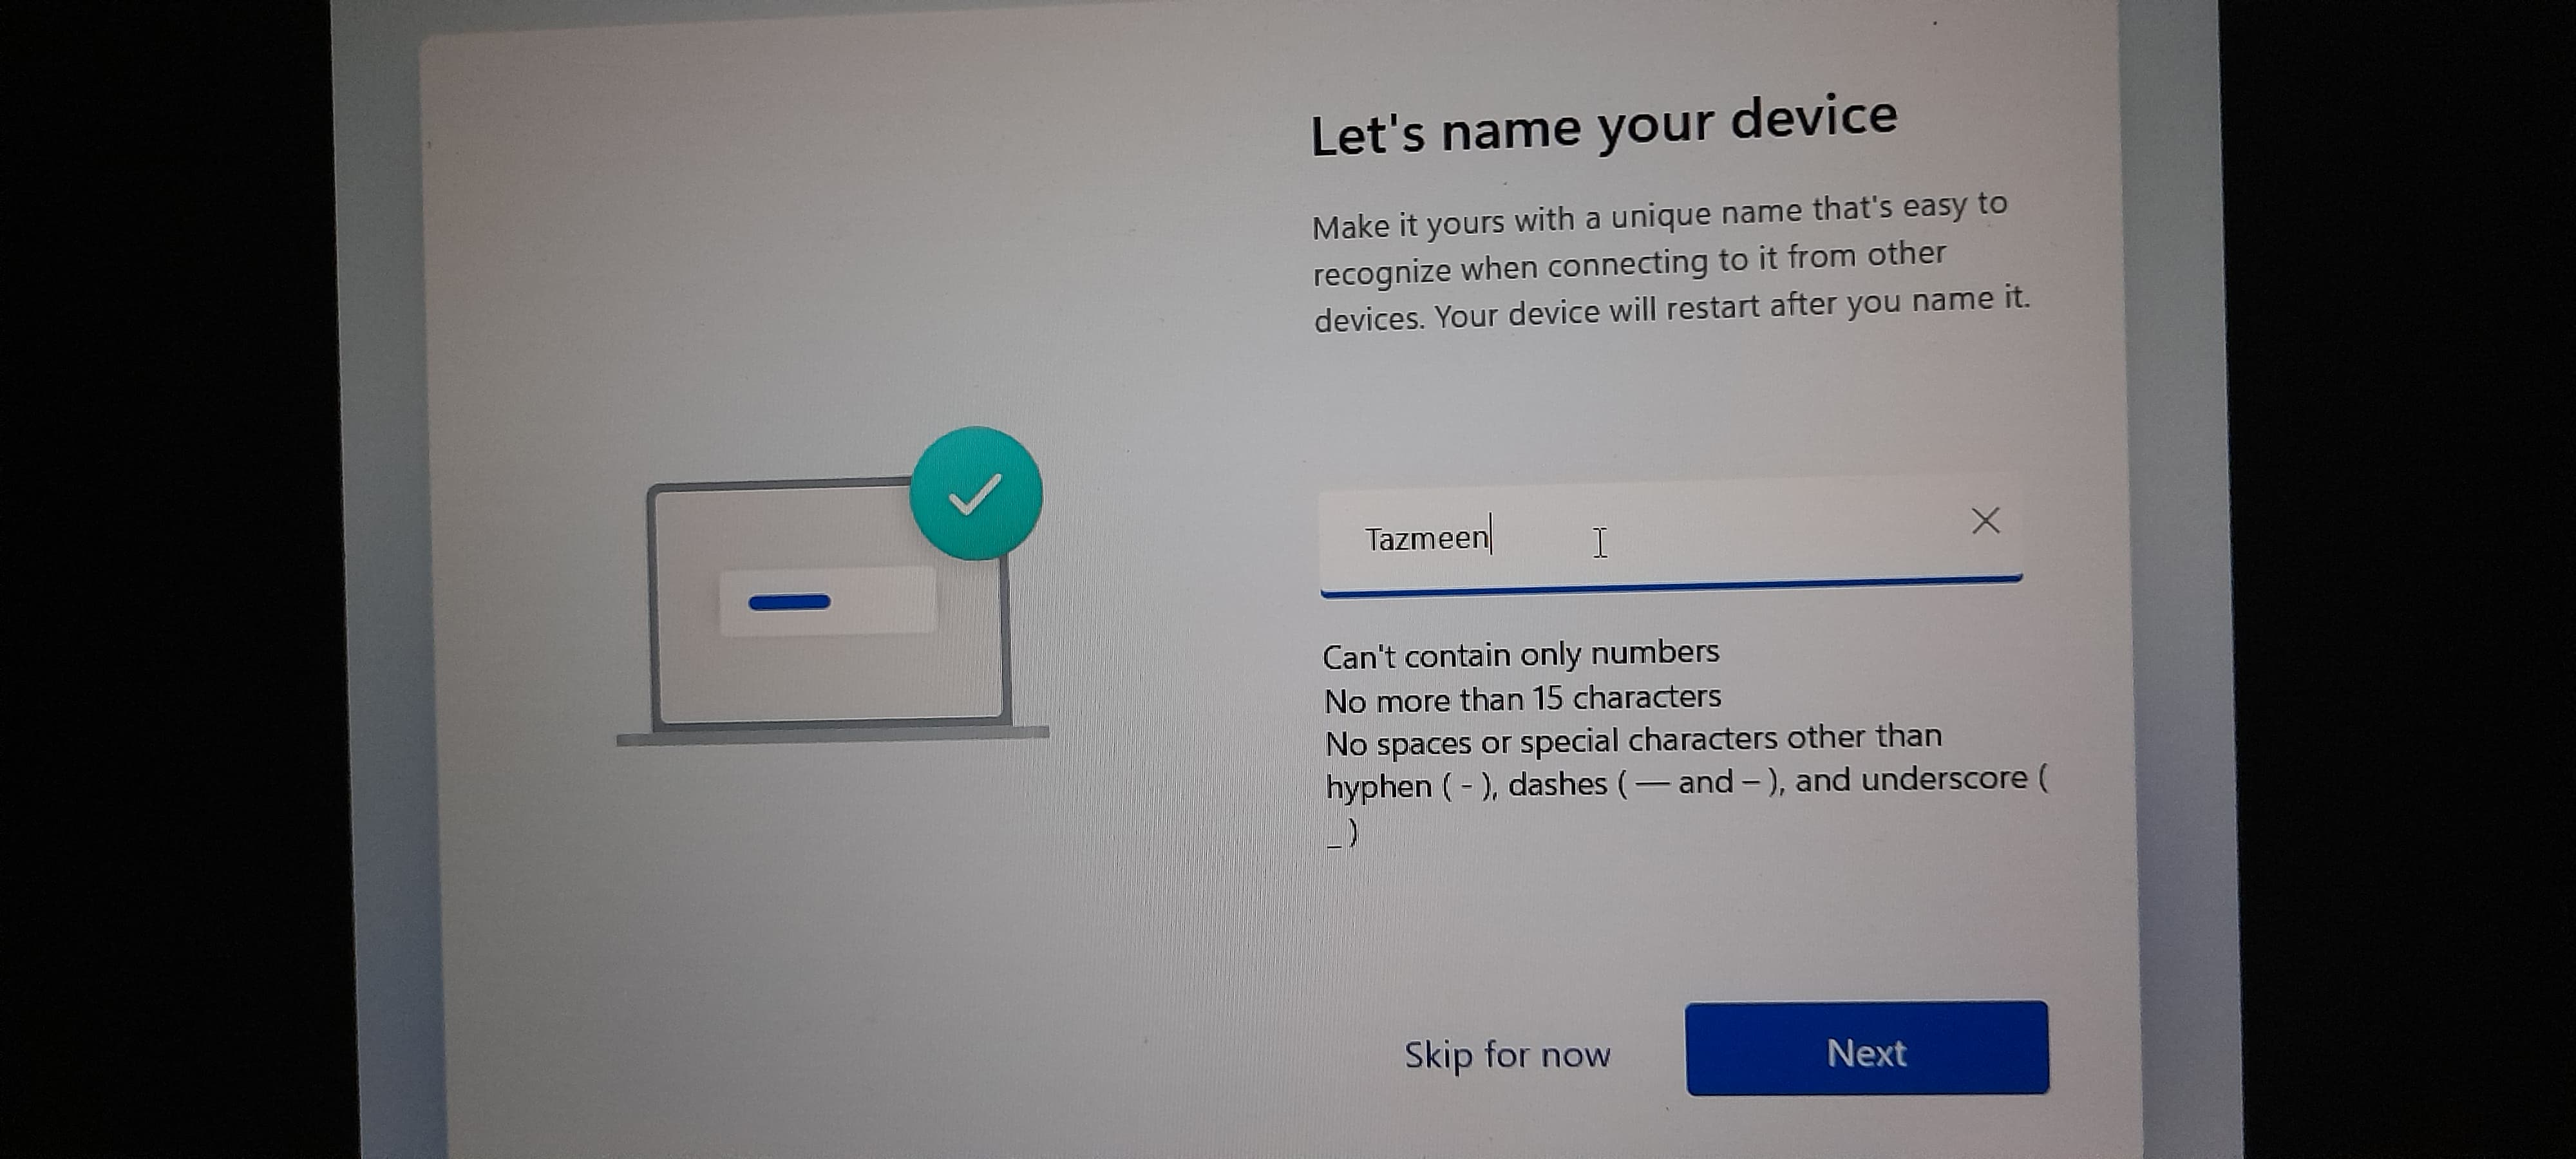
\includegraphics[width=0.8\textwidth]{20.jpeg} % Placeholder for device naming screenshot
    \captionof{figure}{Setup}
\end{center}
\begin{center}
    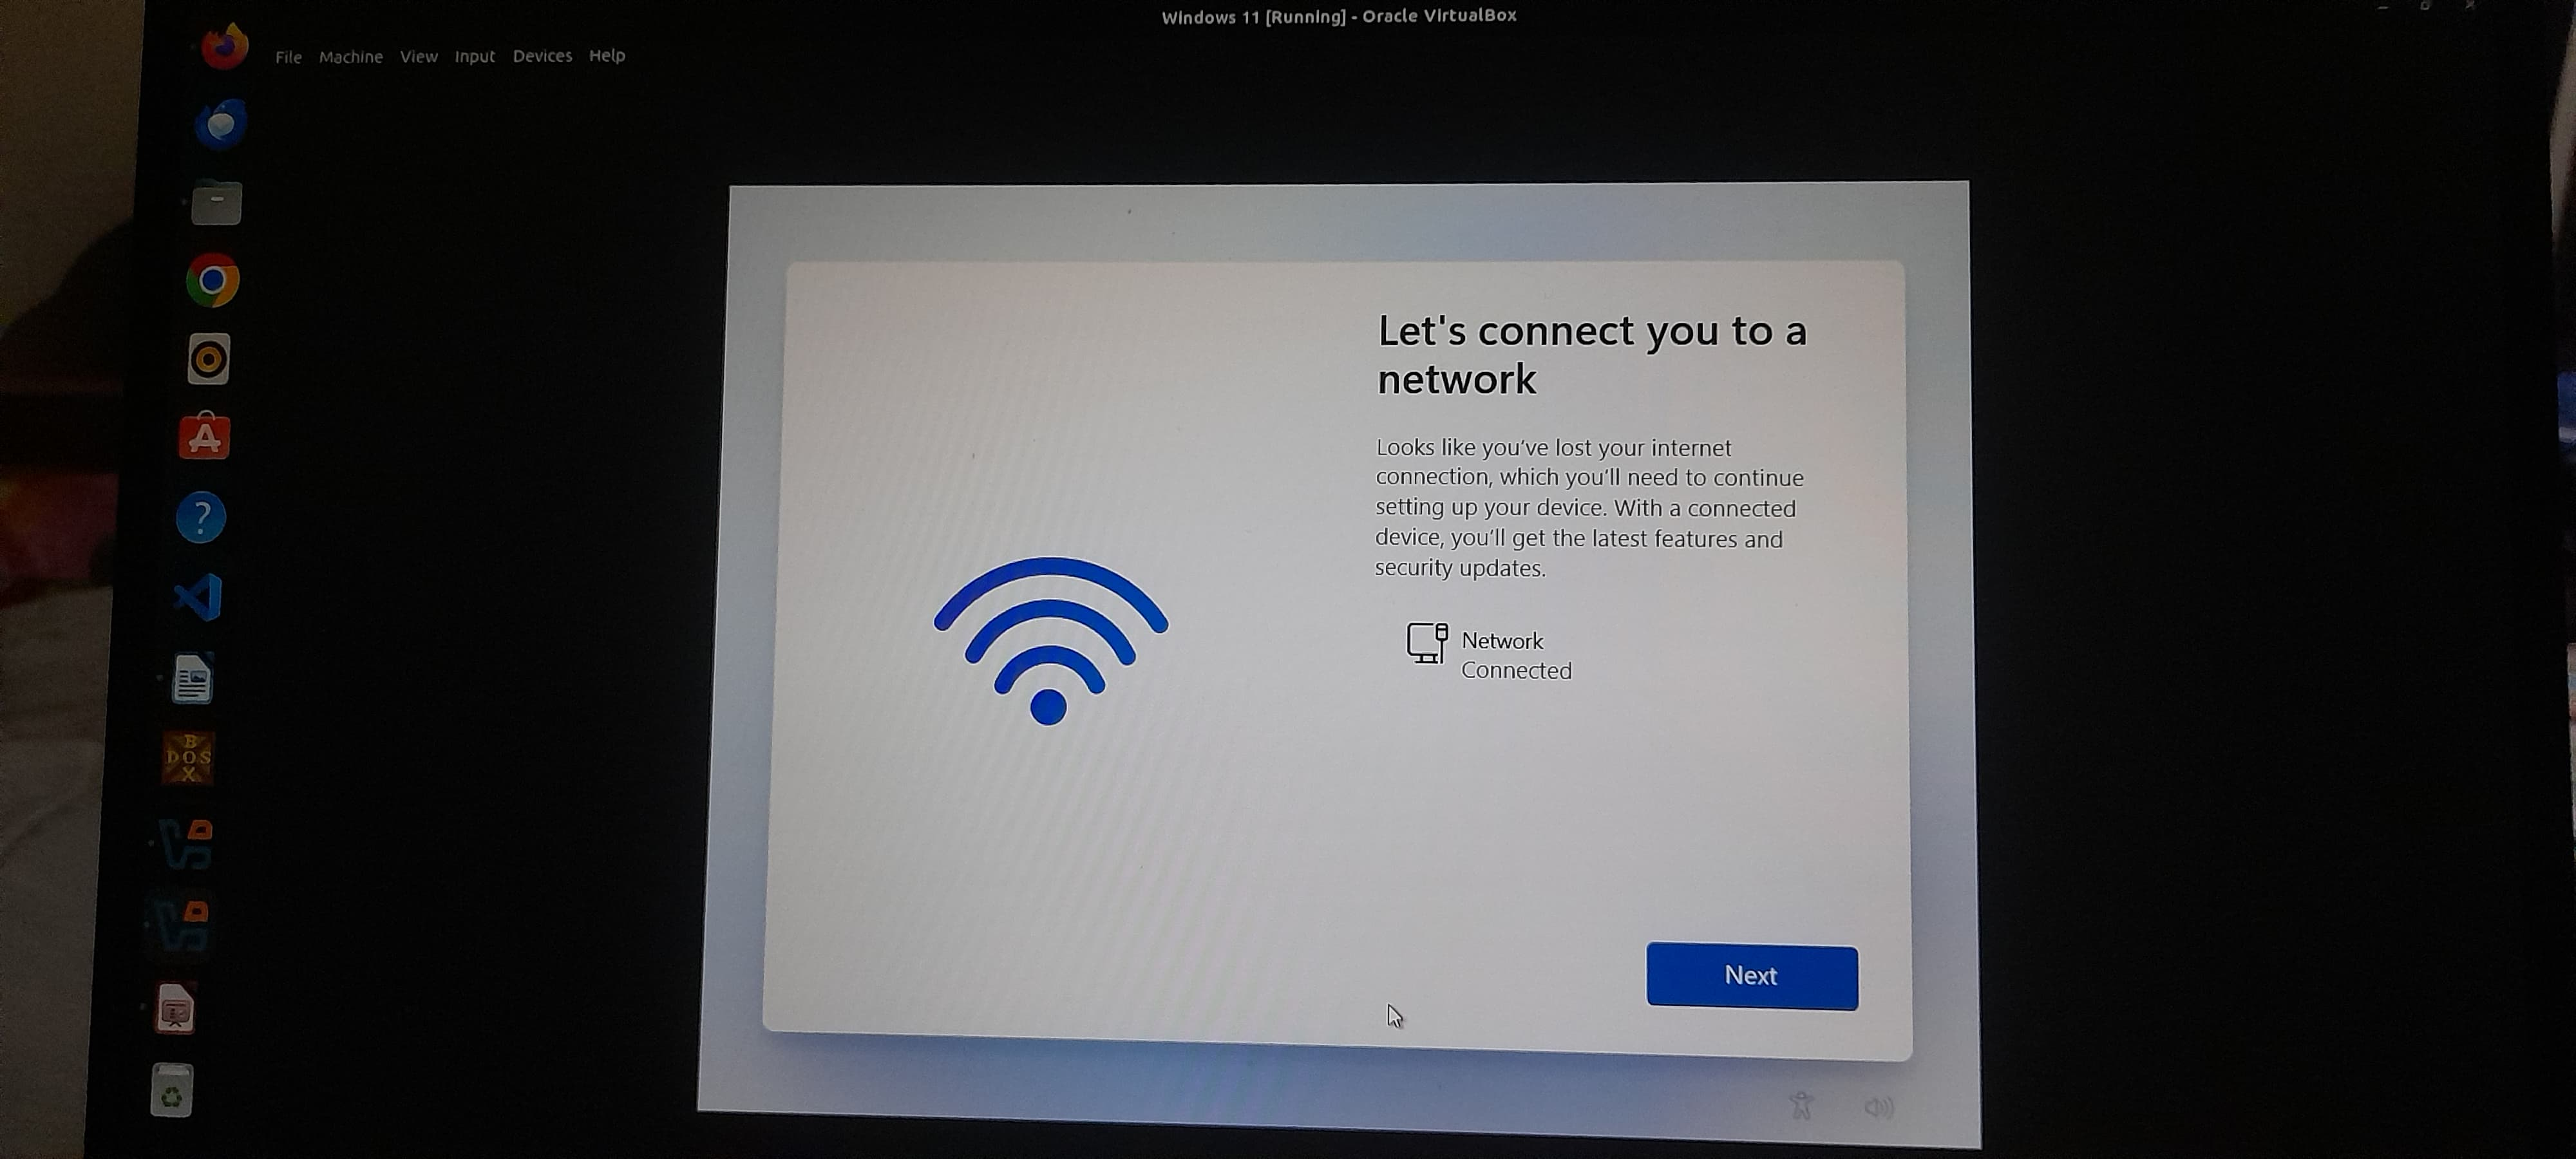
\includegraphics[width=0.8\textwidth]{21.jpeg} % Placeholder for device naming screenshot
    \captionof{figure}{Setup}
\end{center}
\begin{center}
    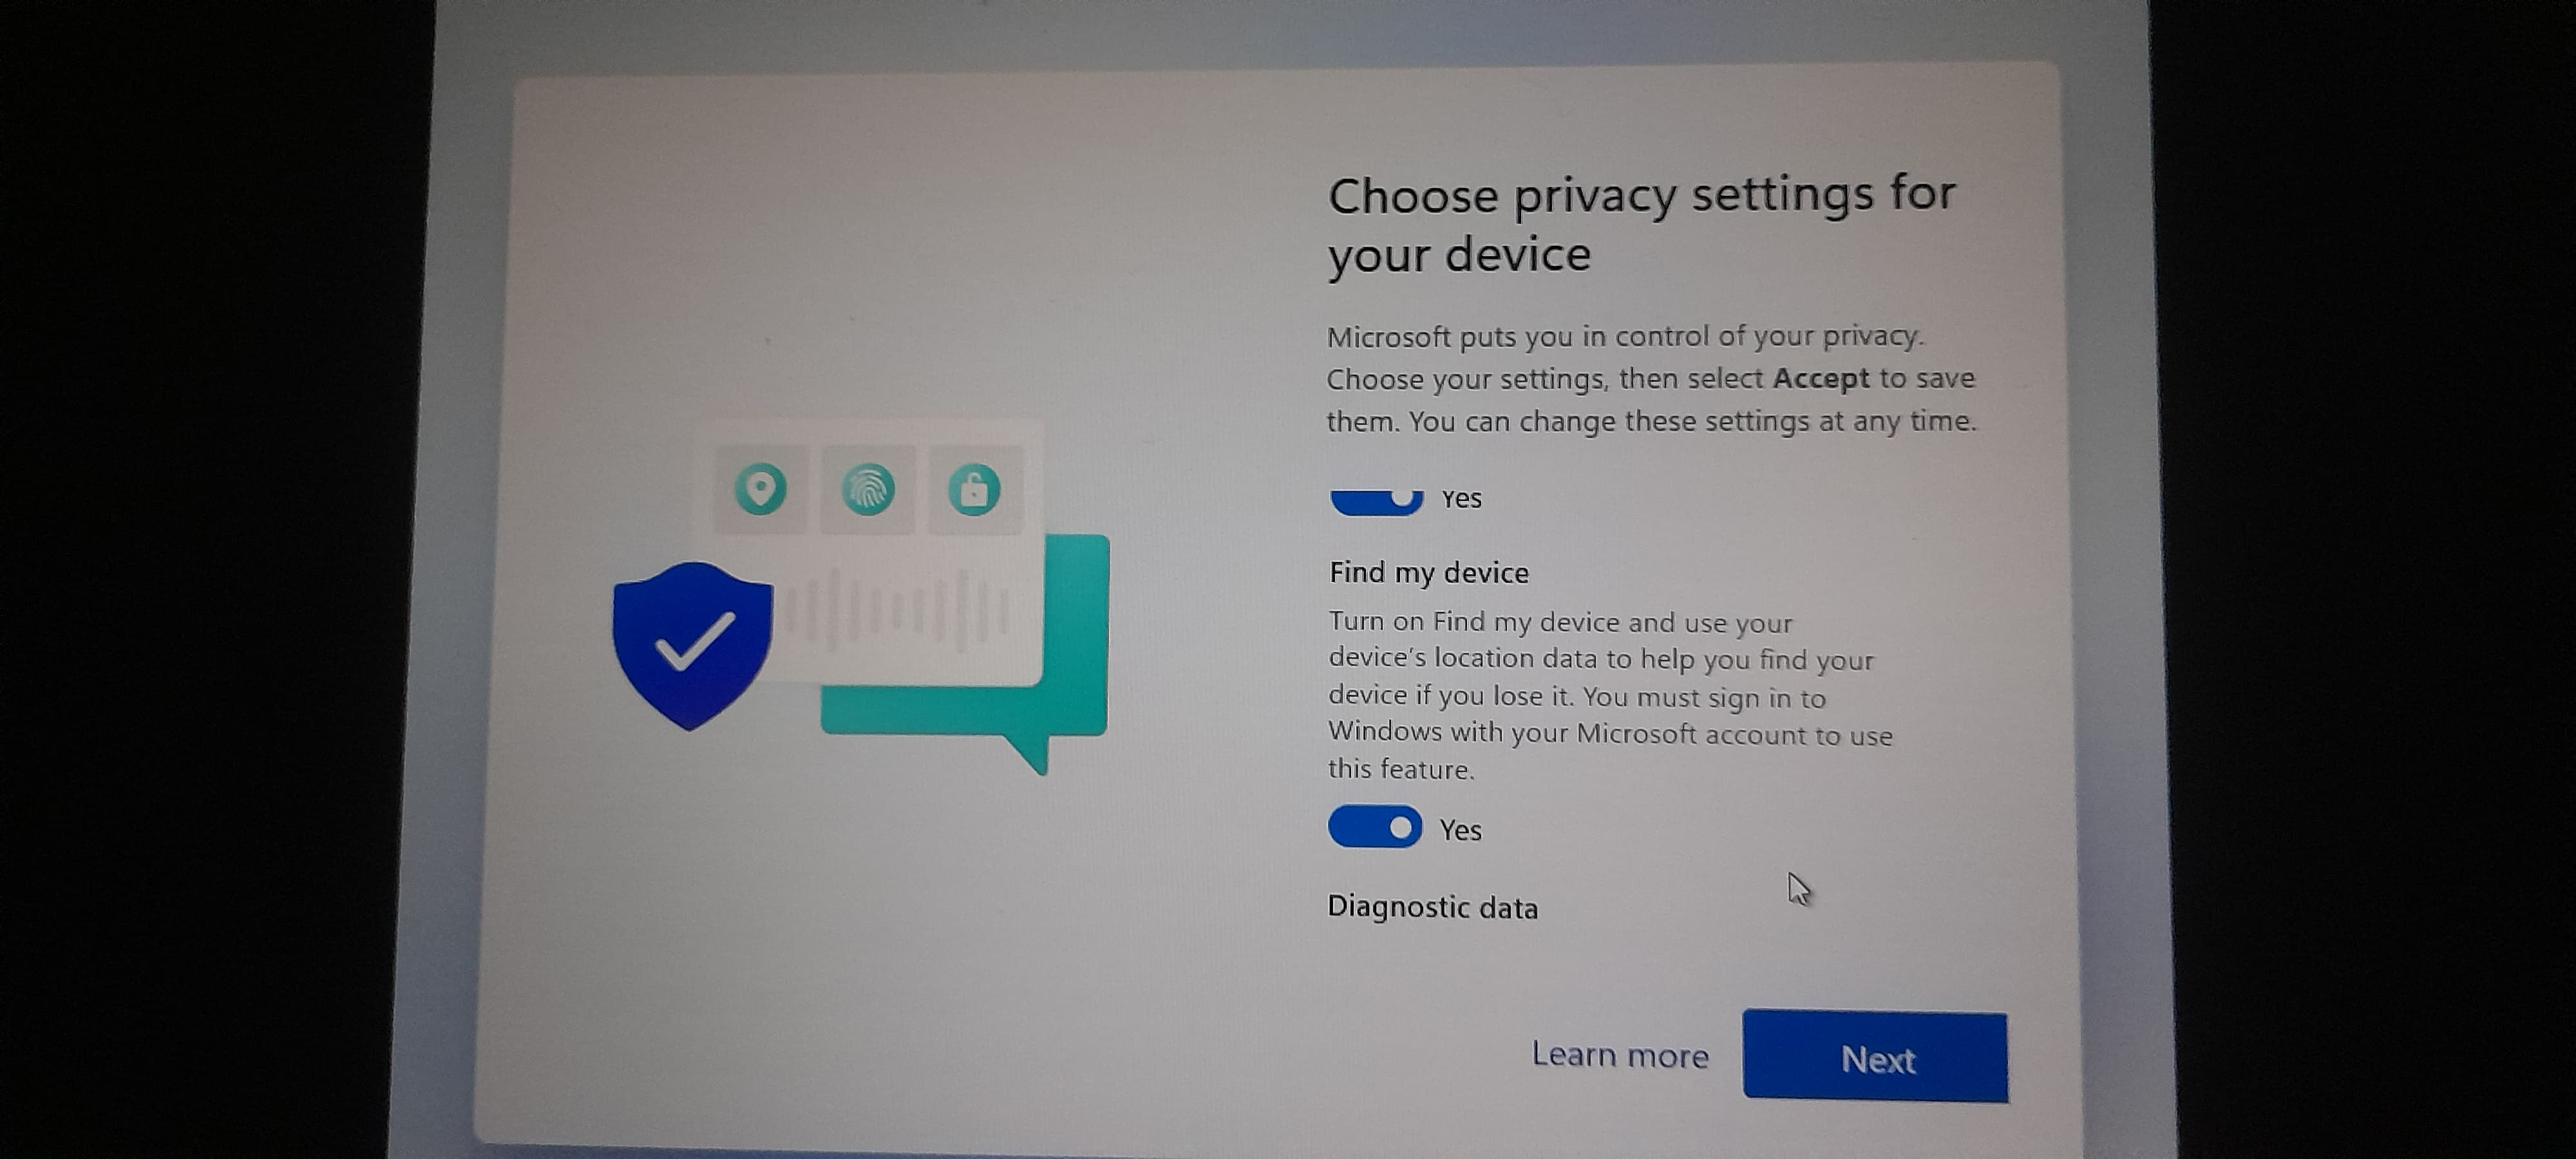
\includegraphics[width=0.8\textwidth]{22.jpeg} % Placeholder for device naming screenshot
    \captionof{figure}{Setup}
\end{center}
\begin{center}
    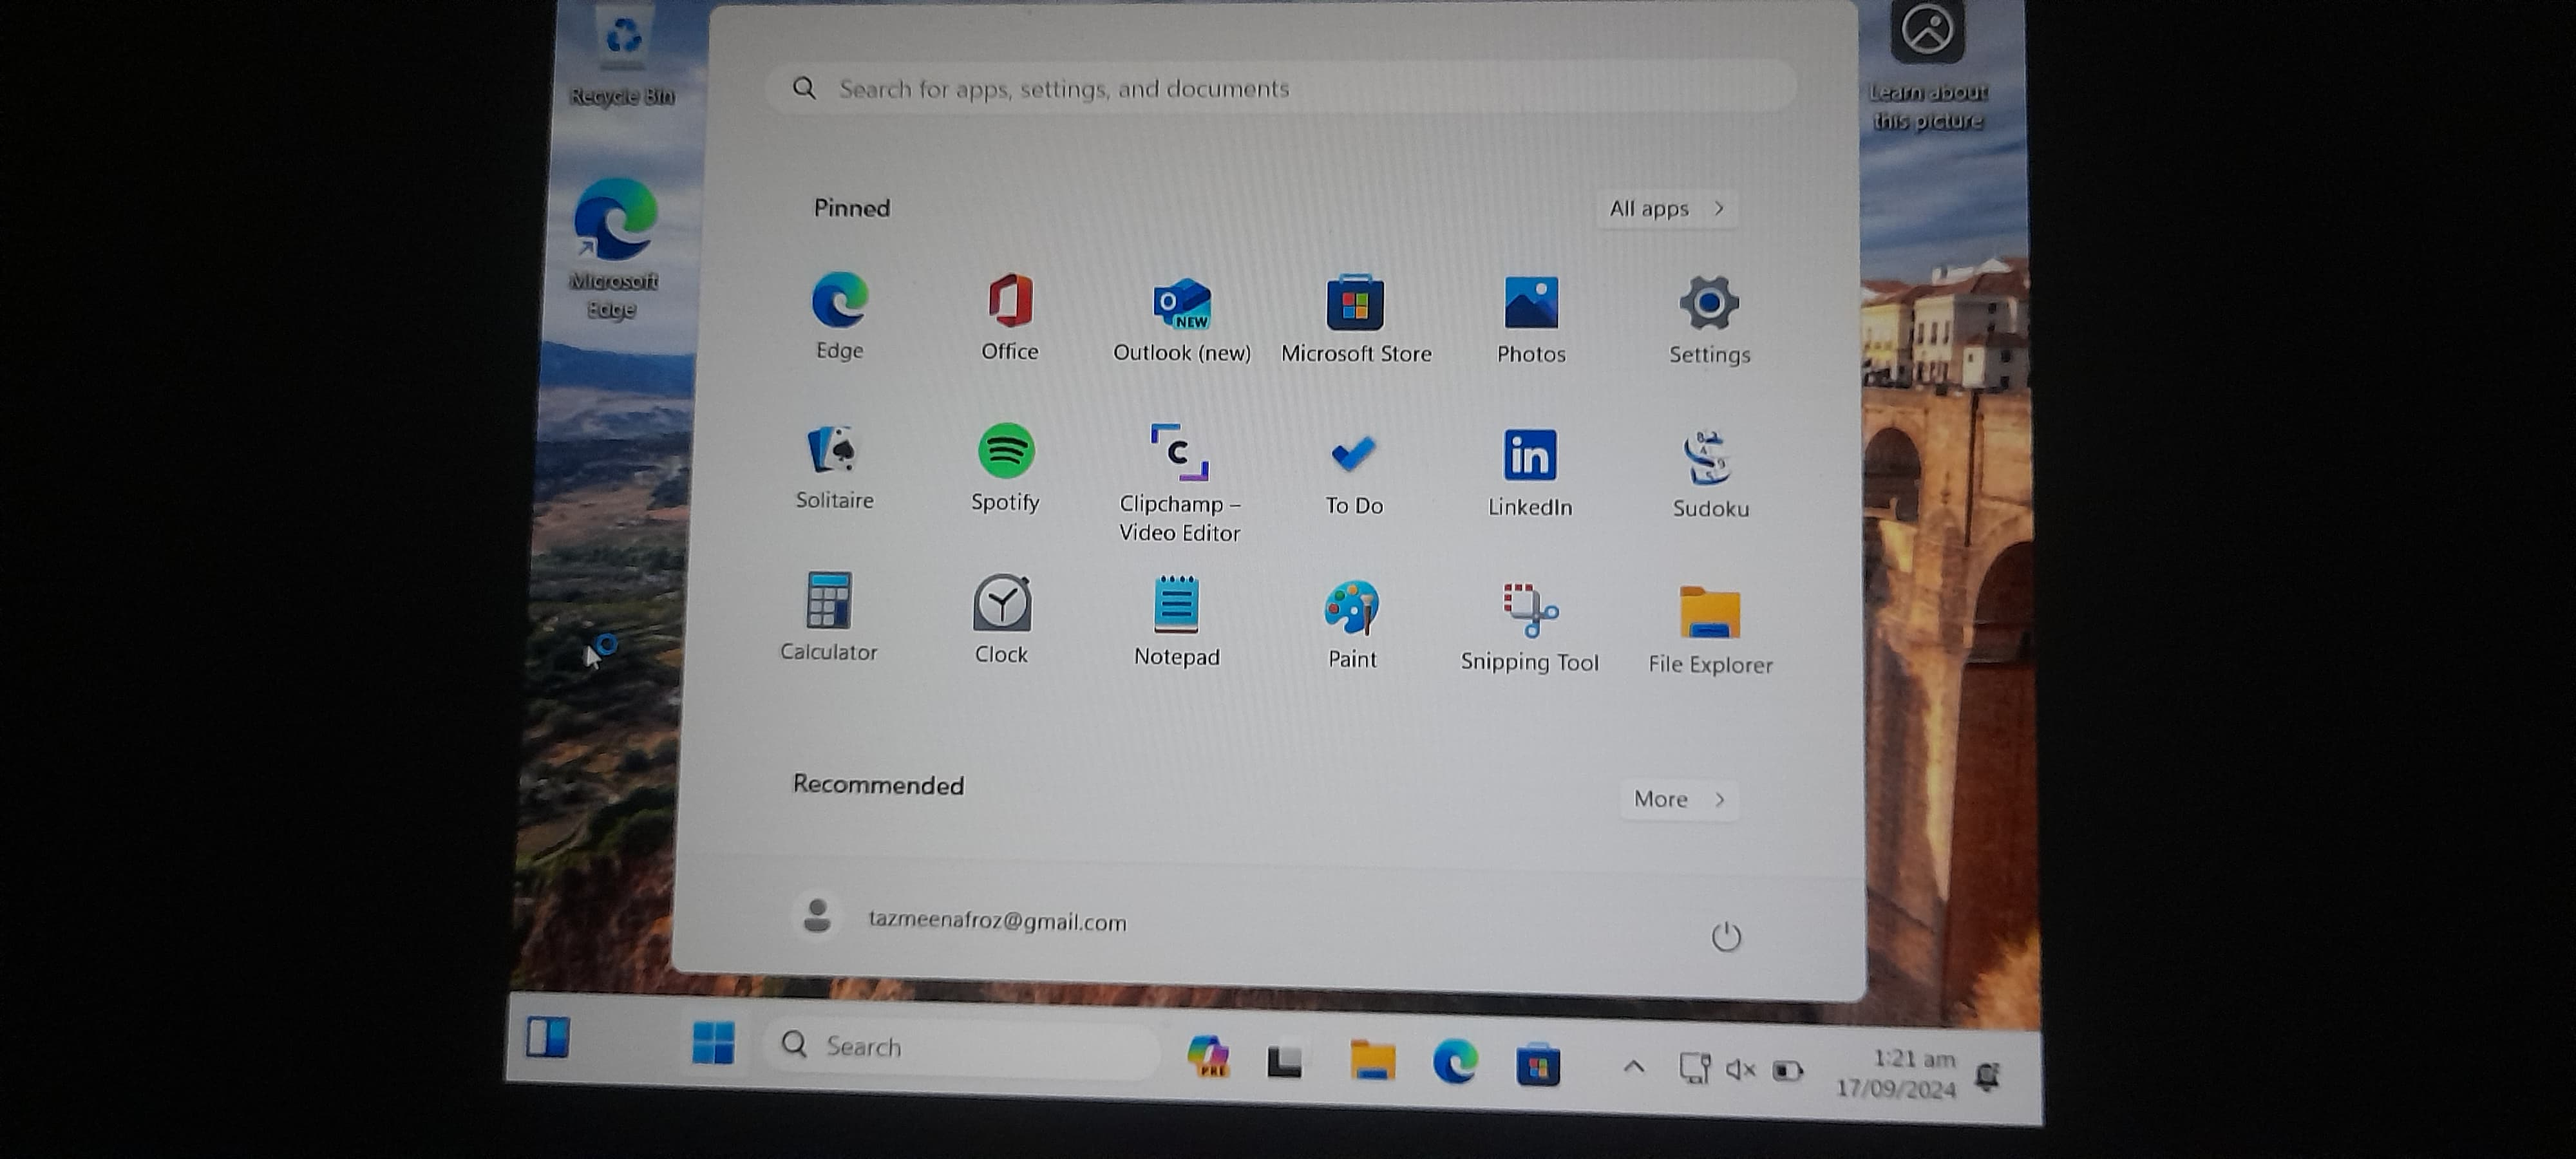
\includegraphics[width=0.8\textwidth]{23.jpeg} % Placeholder for device naming screenshot
    \captionof{figure}{Setup}
\end{center}

\begin{center}
    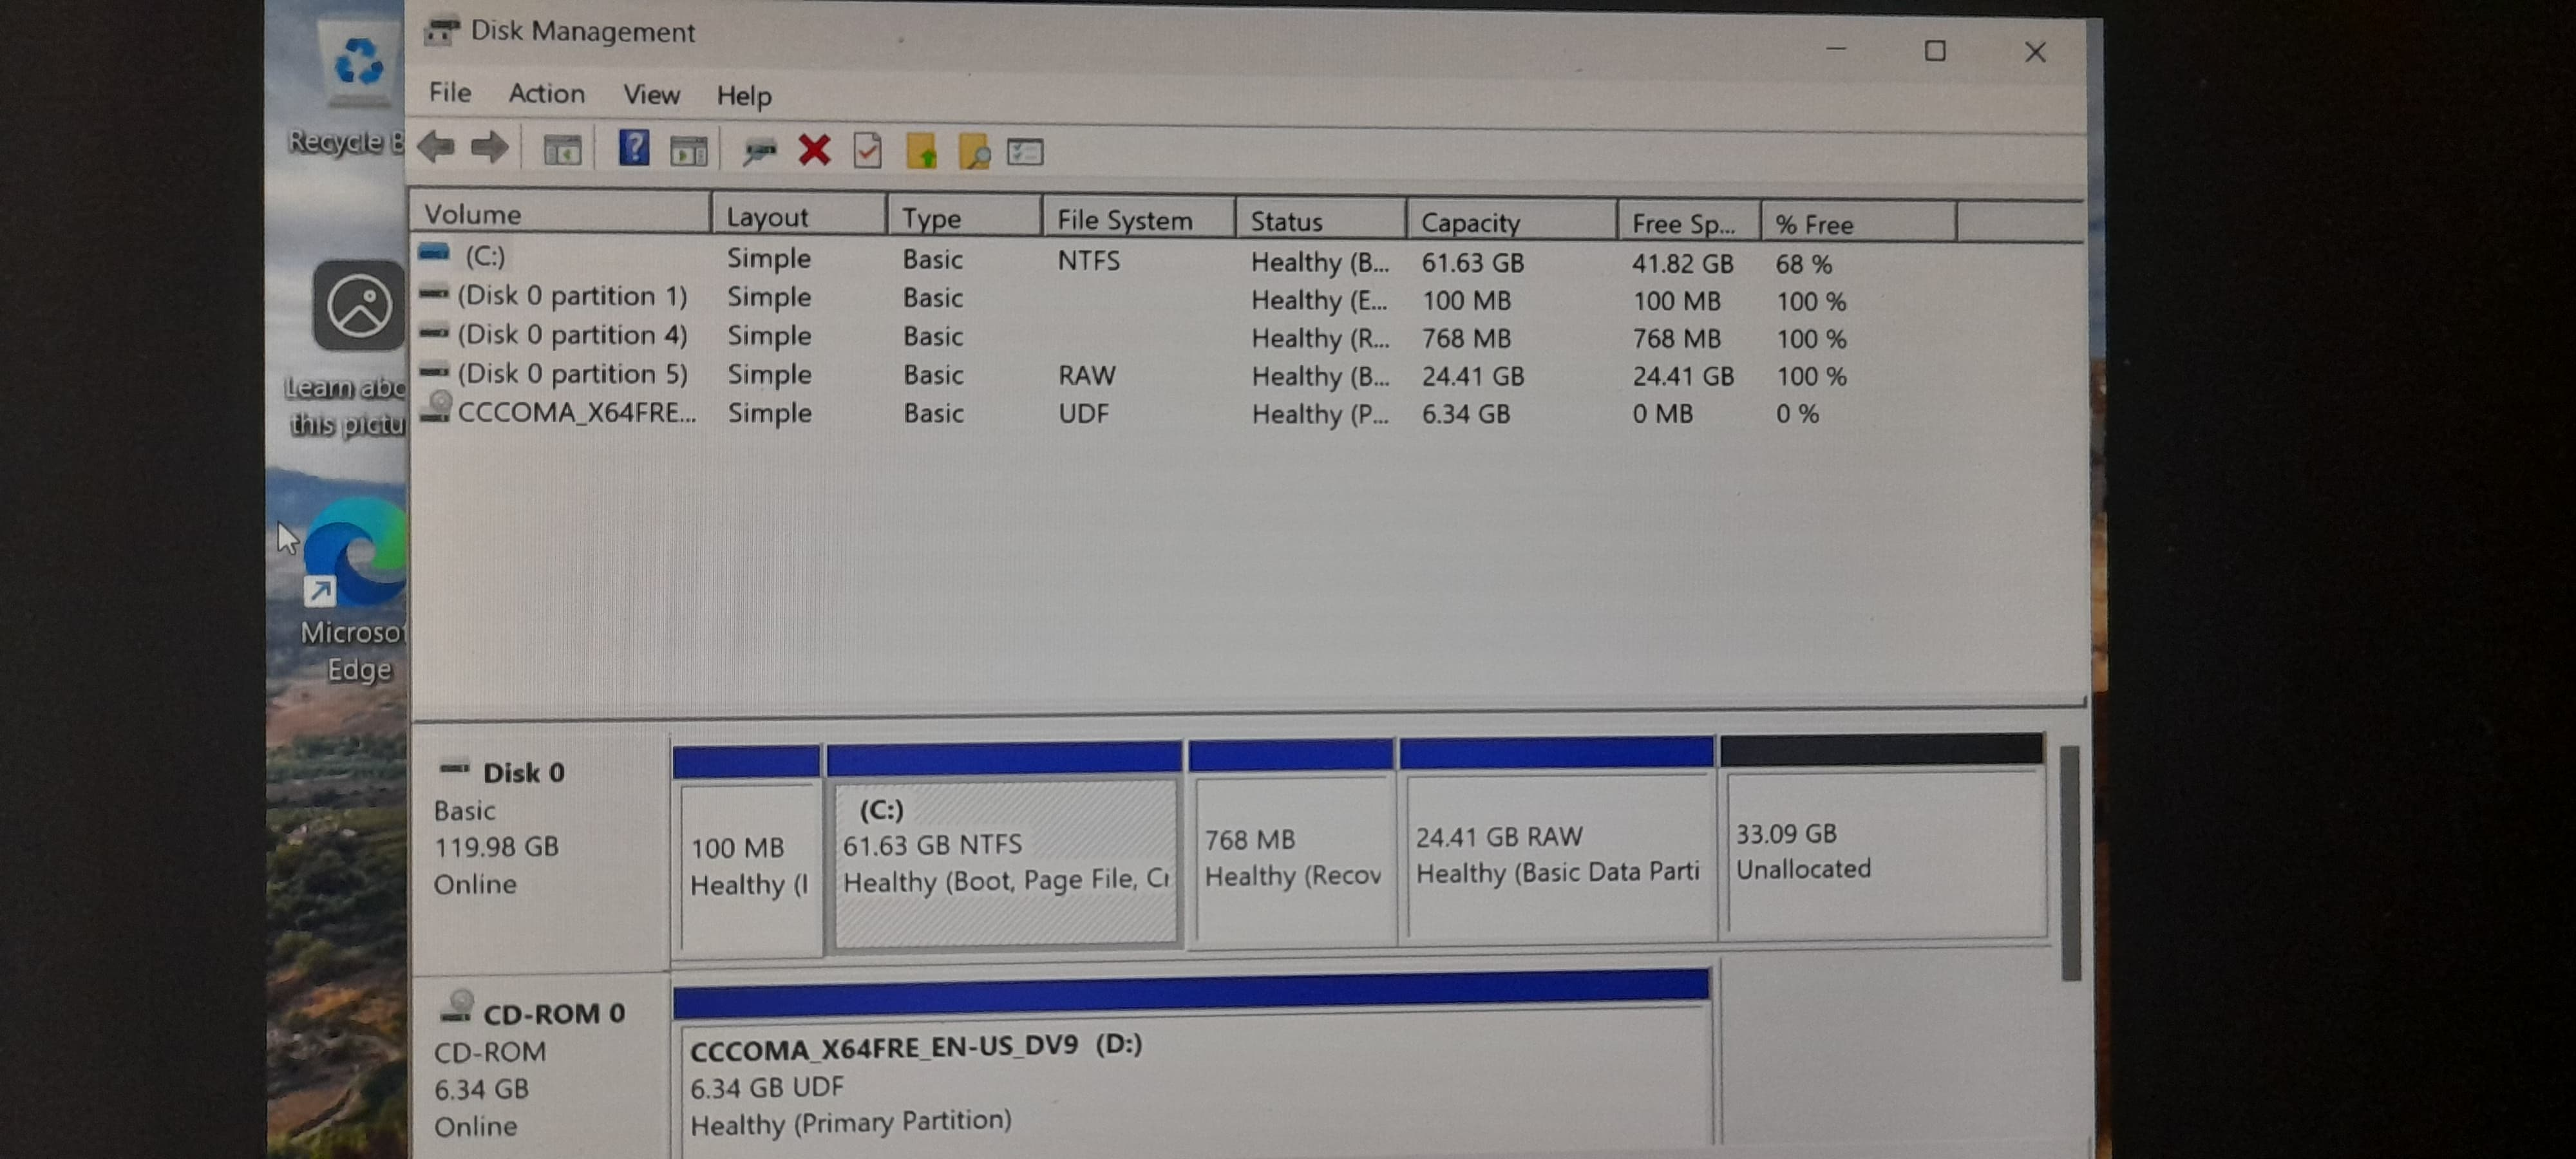
\includegraphics[width=0.8\textwidth]{24.jpeg} % Placeholder for disk management screenshot
    \captionof{figure}{Verifying Partitions in Disk Management}
\end{center}

\section{Installing Arch Linux}
Next, proceed with the installation of Arch Linux using the \texttt{archinstall} command.

\subsection{Arch Installation Process}
Follow the installation wizard and assign the 33GB partition for Arch Linux. 
Select the manual partitioning option and create two partitions: one formatted as ext4 for the root (/) partition and another formatted as FAT32 for the boot (/boot) partition. Set the ext4 partition as root and the FAT32 partition as the boot partition.Configure your user profile, network, and other essential settings.

\begin{center}
    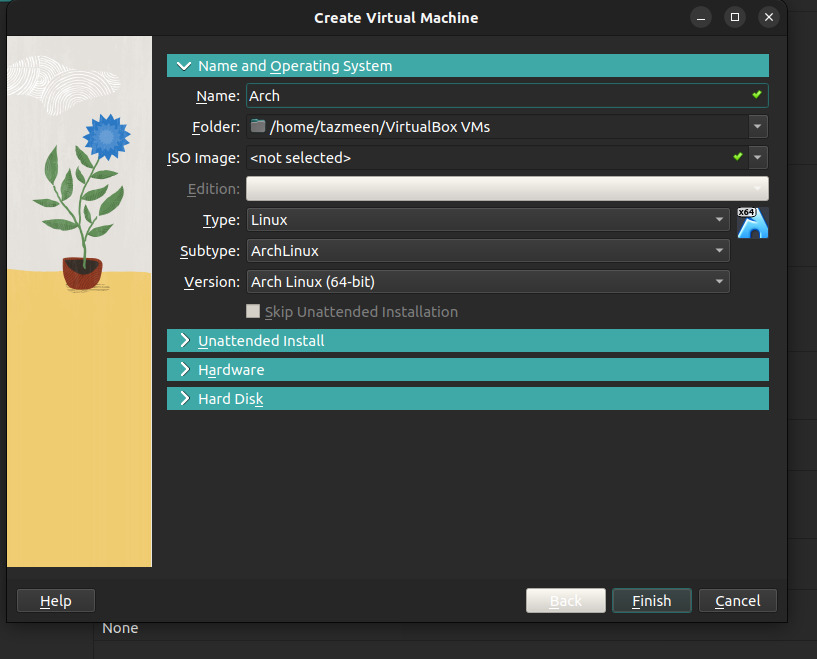
\includegraphics[width=0.8\textwidth]{25.jpeg} % Placeholder for Arch installation screenshot
    \captionof{figure}{Arch Linux Installation Process}
\end{center}
\begin{center}
    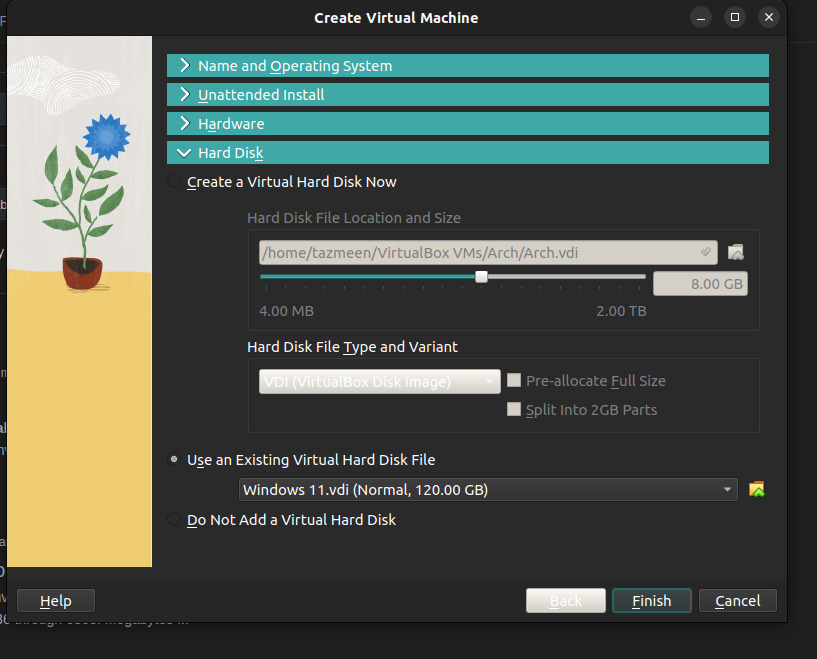
\includegraphics[width=0.8\textwidth]{26.jpeg} % Placeholder for Arch installation screenshot
    \captionof{figure}{Arch Linux Installation Process}
\end{center}
\begin{center}
    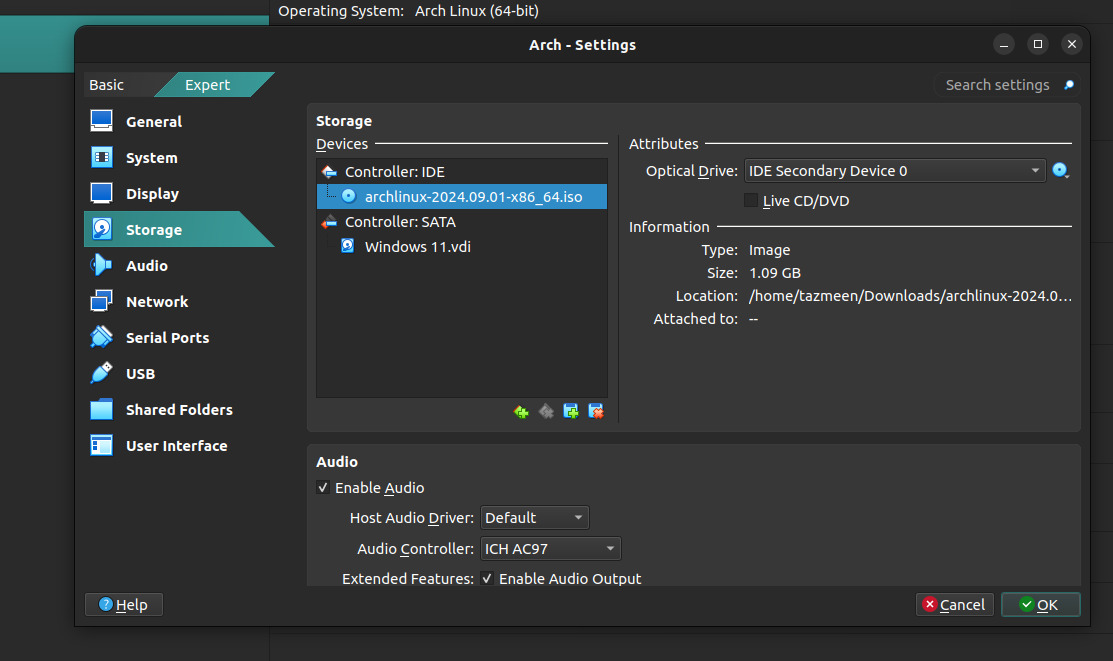
\includegraphics[width=0.8\textwidth]{27.jpeg} % Placeholder for Arch installation screenshot
    \captionof{figure}{Arch Linux Installation Process}
\end{center}
\begin{center}
    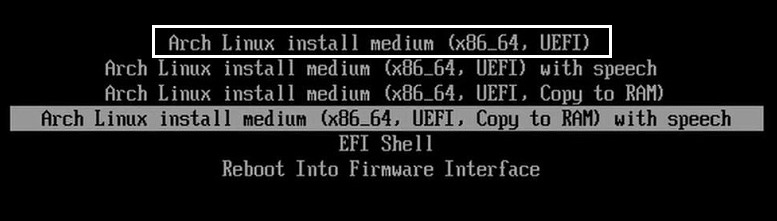
\includegraphics[width=0.8\textwidth]{28.jpeg} % Placeholder for Arch installation screenshot
    \captionof{figure}{Arch Linux Installation Process}
\end{center}
\begin{center}
    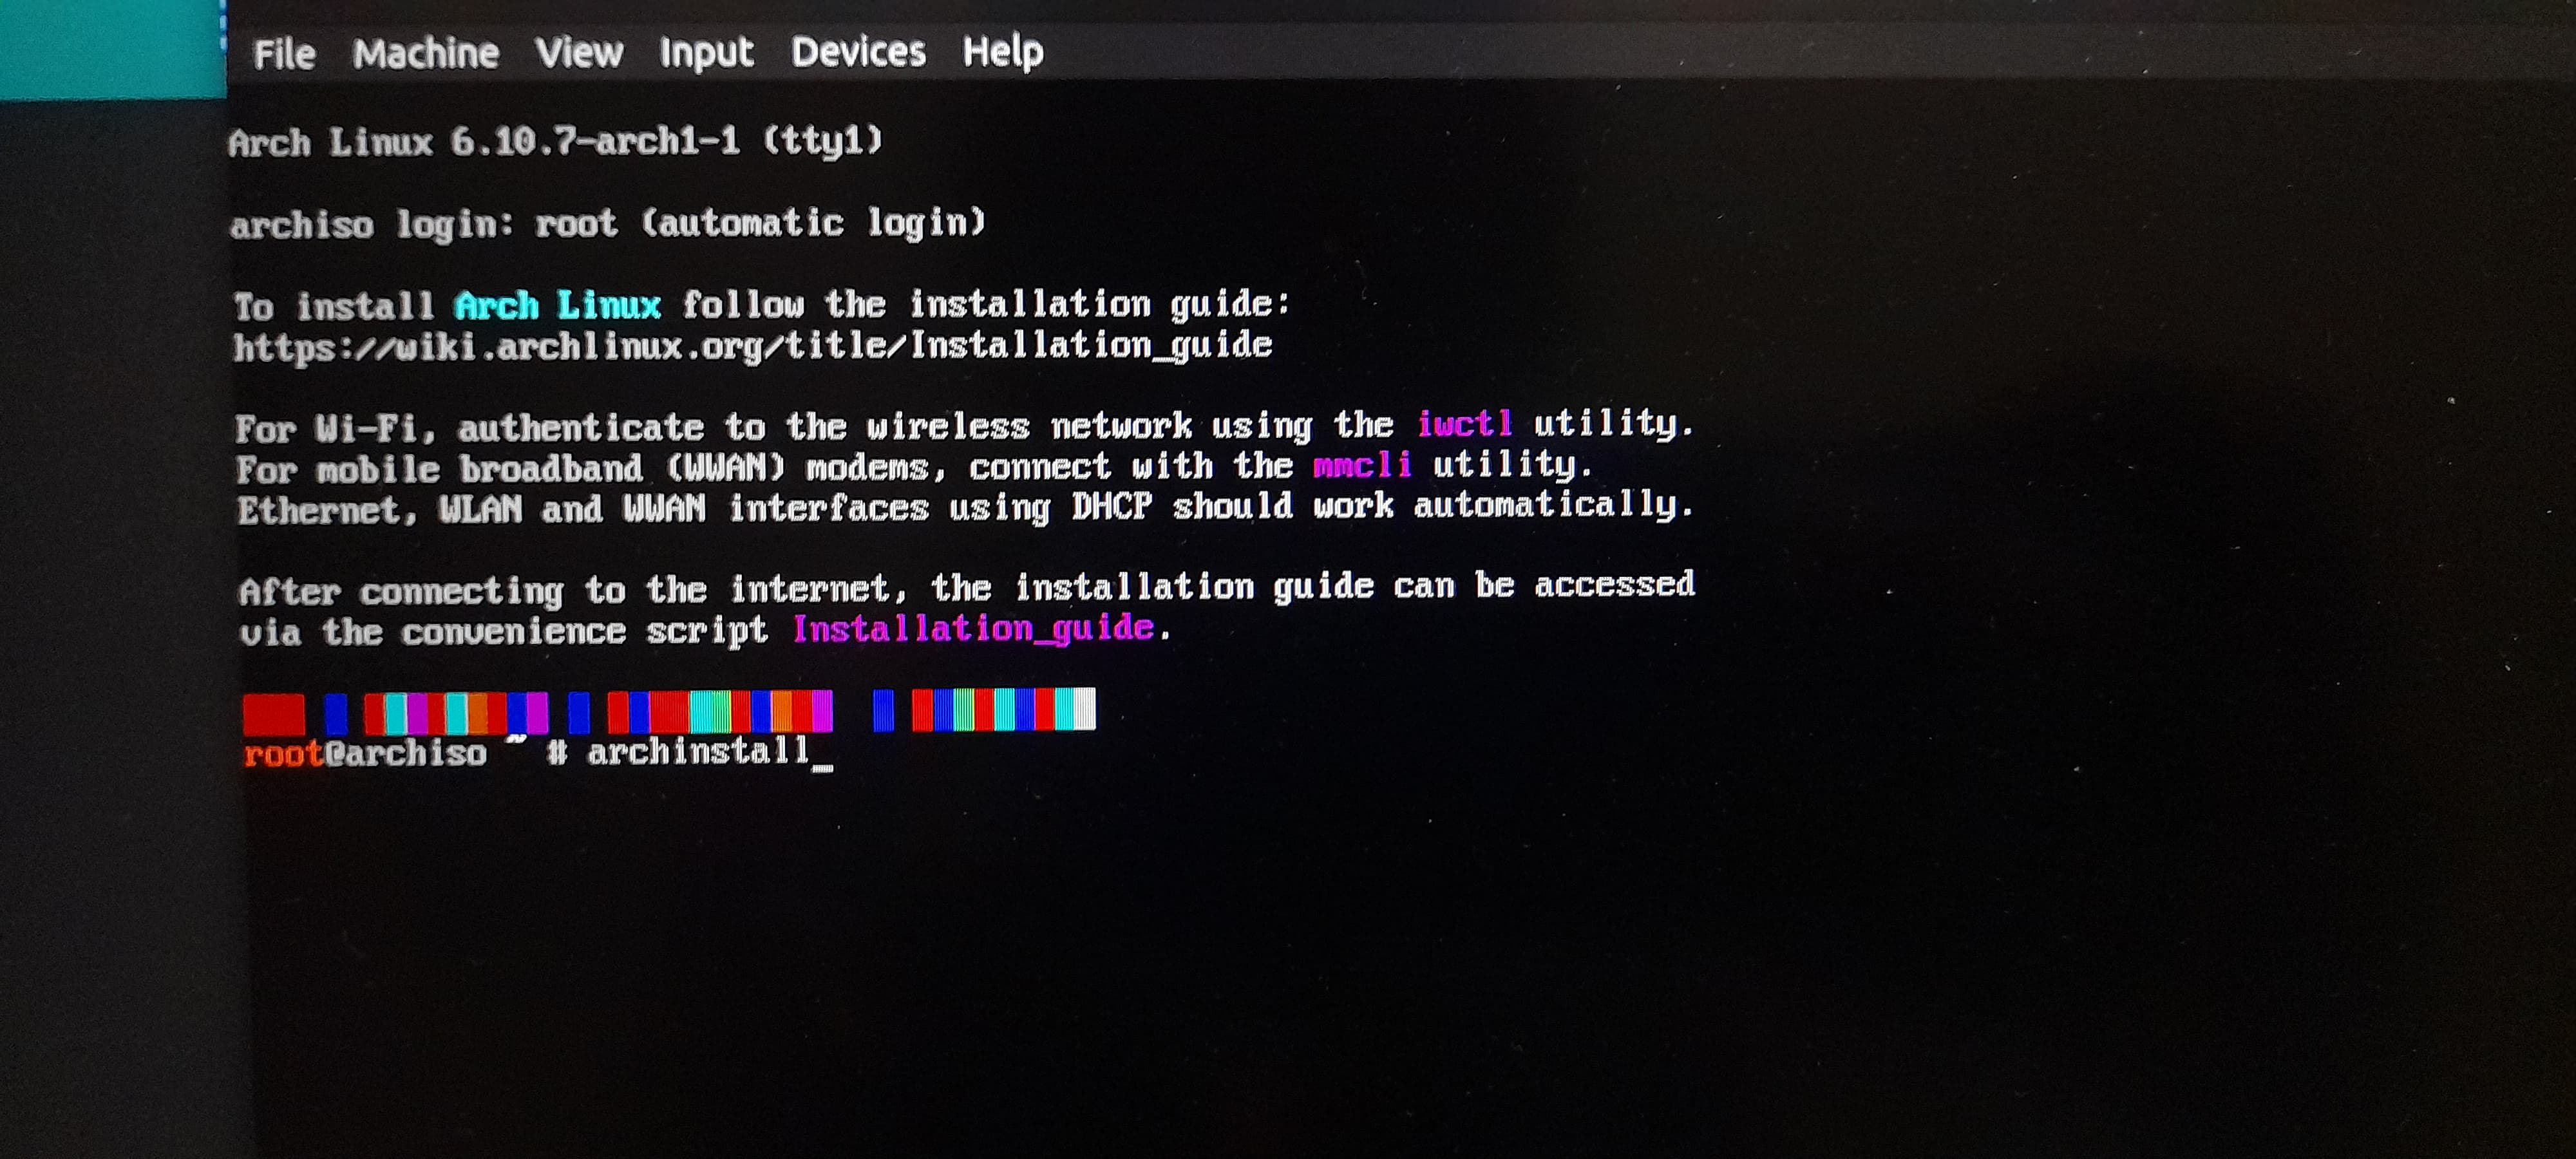
\includegraphics[width=0.8\textwidth]{29.jpeg} % Placeholder for Arch installation screenshot
    \captionof{figure}{Arch Linux Installation Process}
\end{center}
\begin{center}
    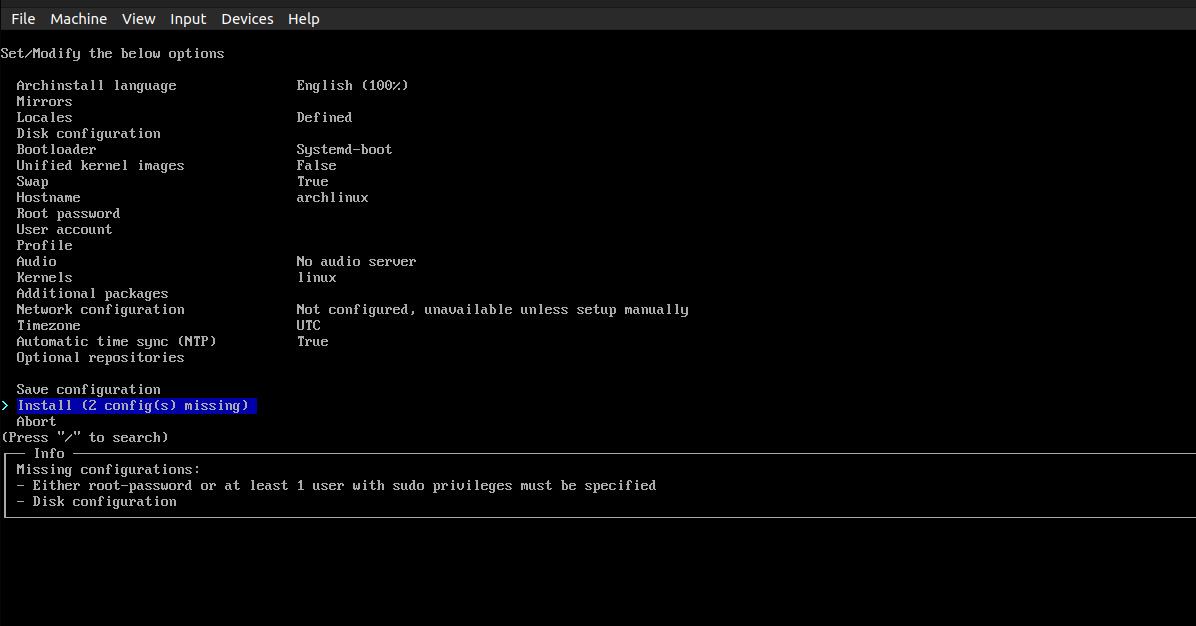
\includegraphics[width=0.8\textwidth]{30.jpeg} % Placeholder for Arch installation screenshot
    \captionof{figure}{Arch Linux Installation Process}
\end{center}
\begin{center}
    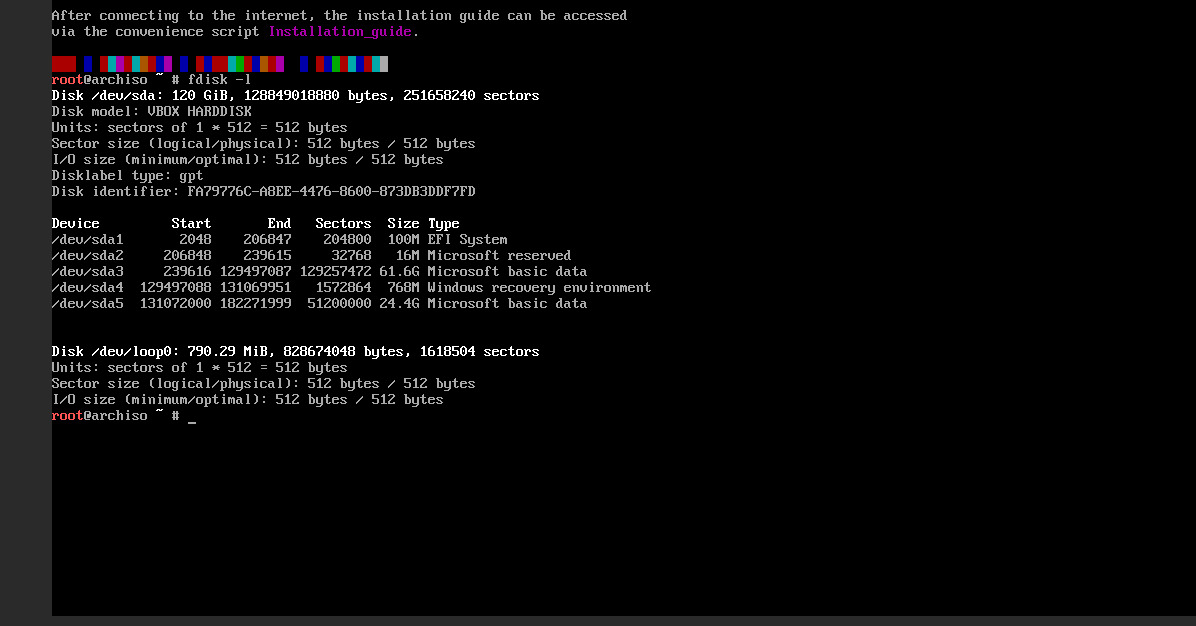
\includegraphics[width=0.8\textwidth]{31.jpeg} % Placeholder for Arch installation screenshot
    \captionof{figure}{Arch Linux Installation Process}
\end{center}
\begin{center}
    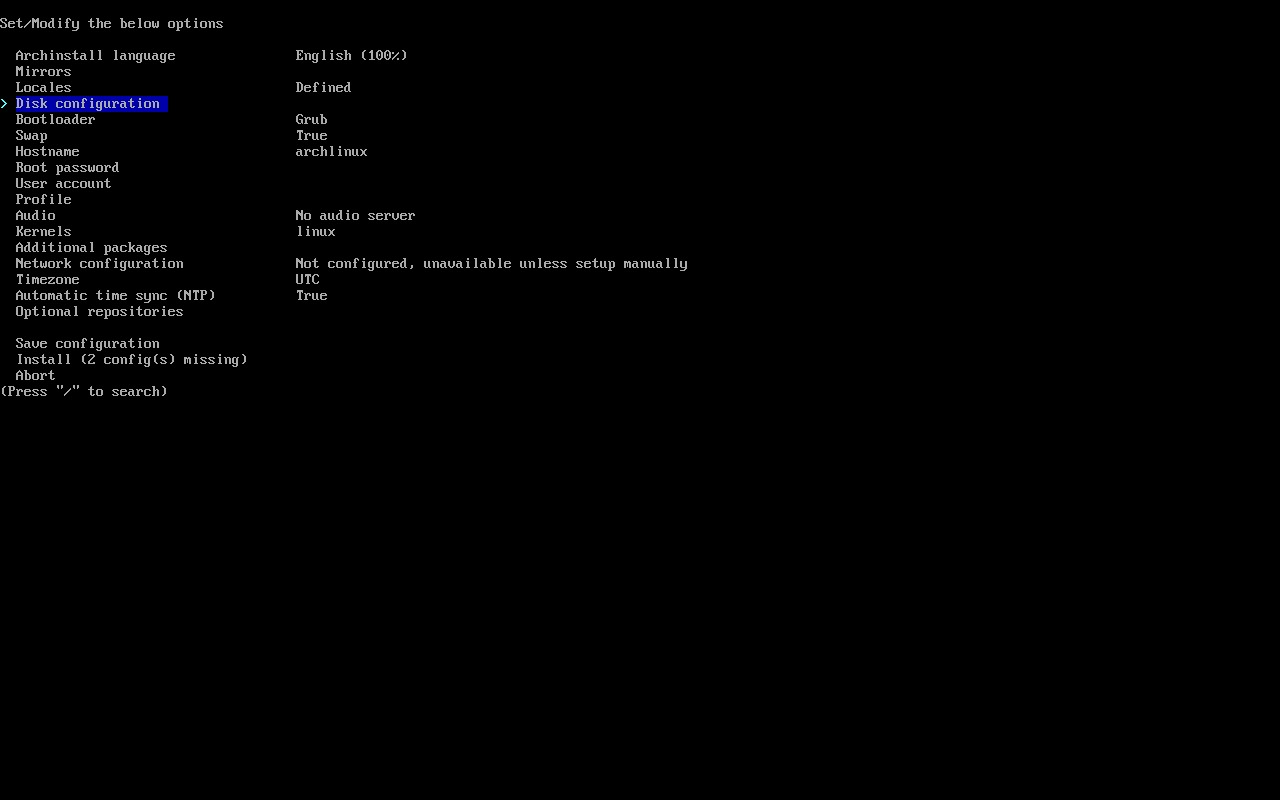
\includegraphics[width=0.8\textwidth]{32.jpeg} % Placeholder for Arch installation screenshot
    \captionof{figure}{Arch Linux Installation Process}
\end{center}
\begin{center}
    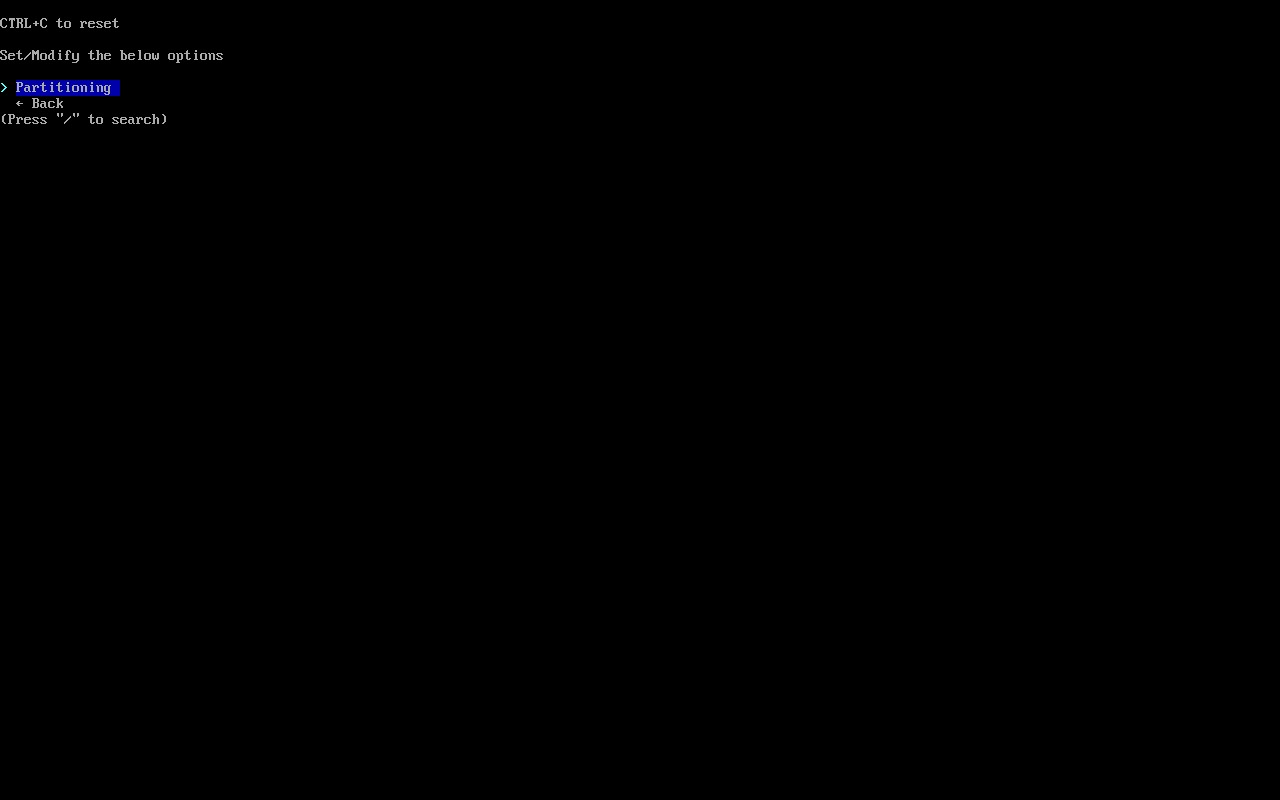
\includegraphics[width=0.8\textwidth]{33.jpeg} % Placeholder for Arch installation screenshot
    \captionof{figure}{Arch Linux Installation Process}
\end{center}\begin{center}
    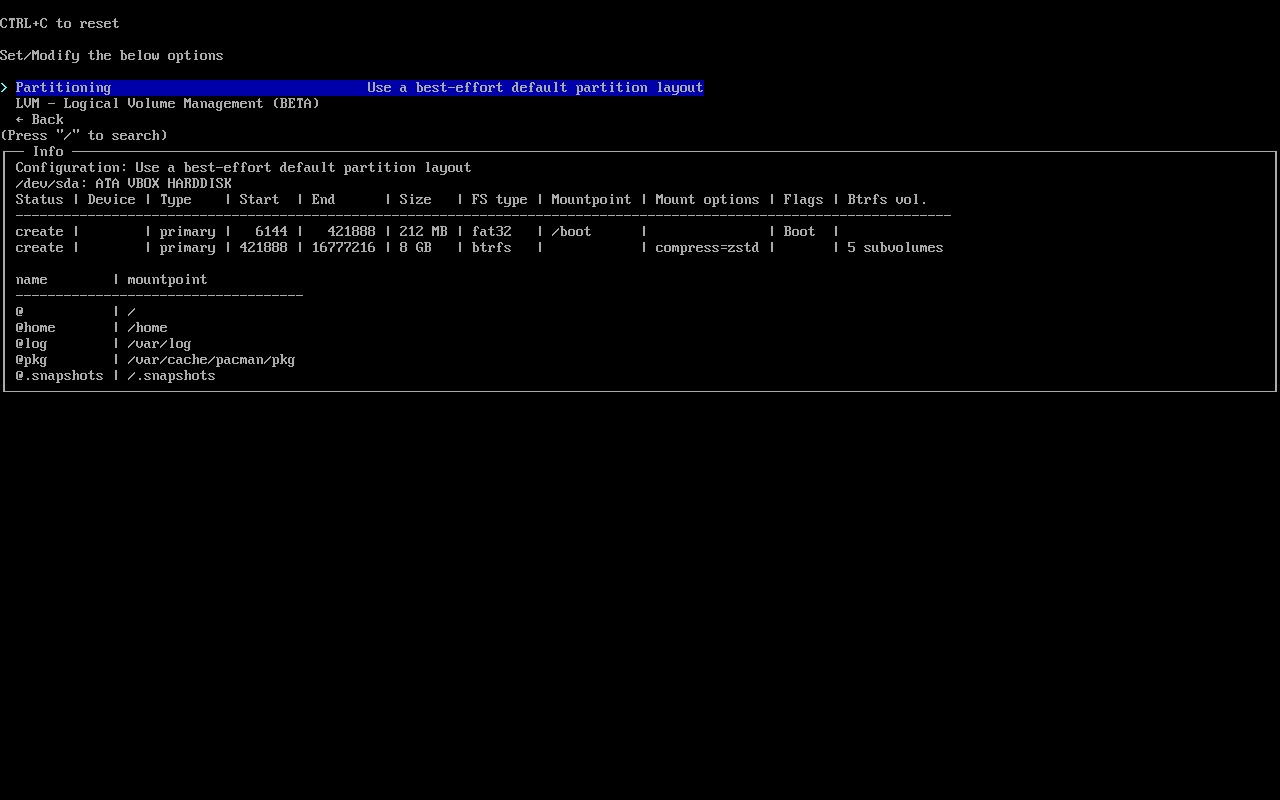
\includegraphics[width=0.8\textwidth]{34.jpeg} % Placeholder for Arch installation screenshot
    \captionof{figure}{Arch Linux Installation Process}
\end{center}
\begin{center}
    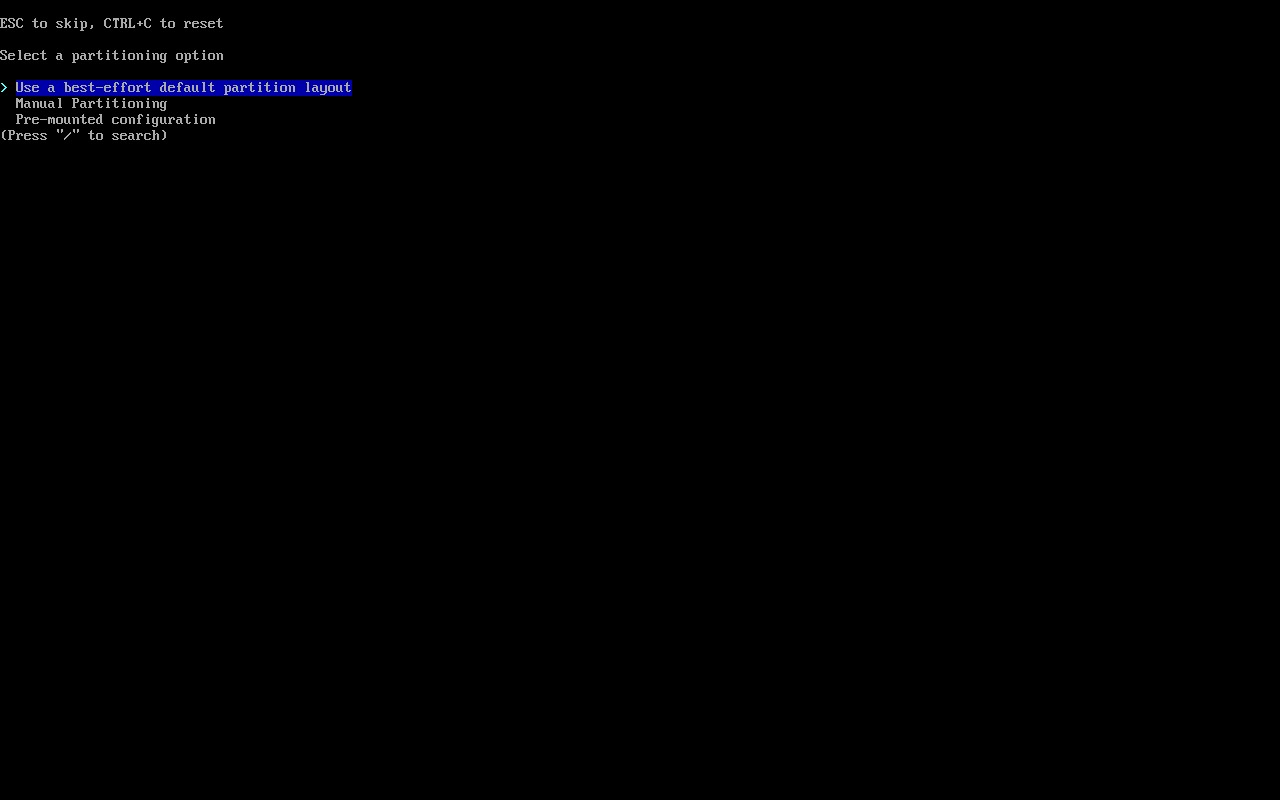
\includegraphics[width=0.8\textwidth]{35.jpeg} % Placeholder for Arch installation screenshot
    \captionof{figure}{Arch Linux Installation Process}
\end{center}
\begin{center}
    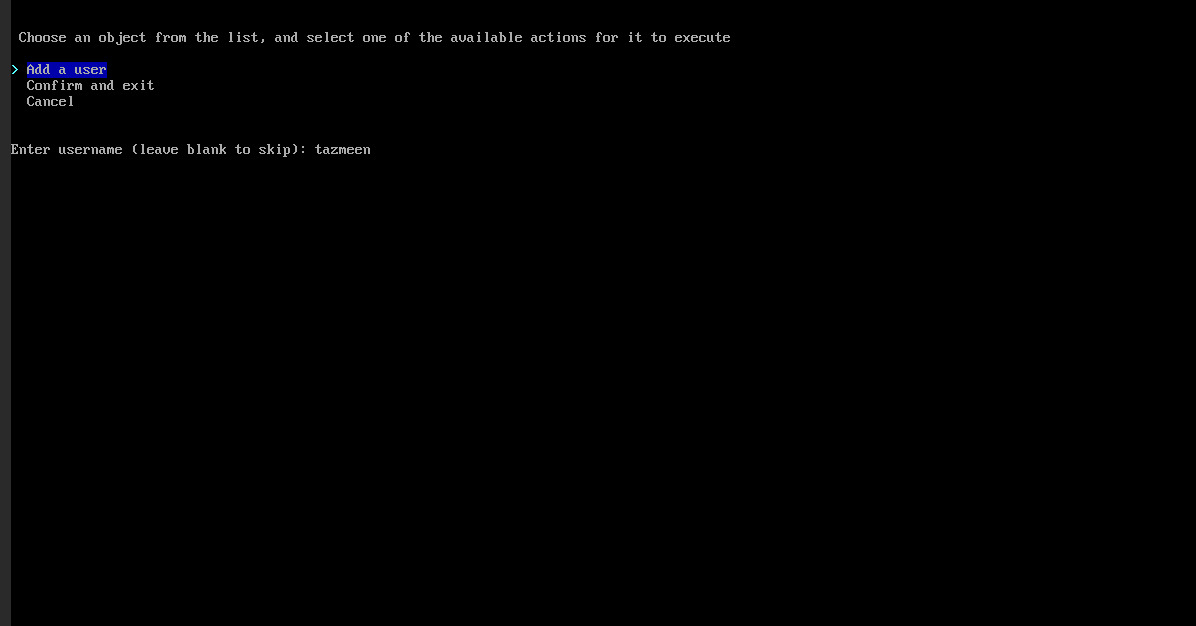
\includegraphics[width=0.8\textwidth]{36.jpeg} % Placeholder for Arch installation screenshot
    \captionof{figure}{Arch Linux Installation Process}
\end{center}
\begin{center}
    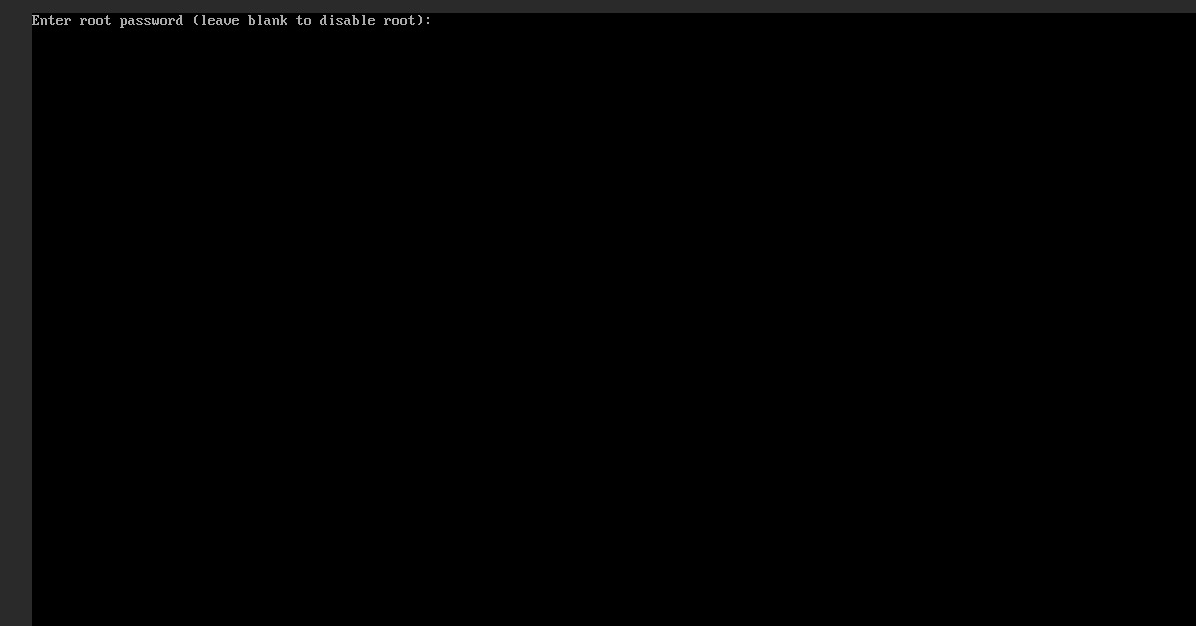
\includegraphics[width=0.8\textwidth]{37.jpeg} % Placeholder for Arch installation screenshot
    \captionof{figure}{Arch Linux Installation Process}
\end{center}
\begin{center}
    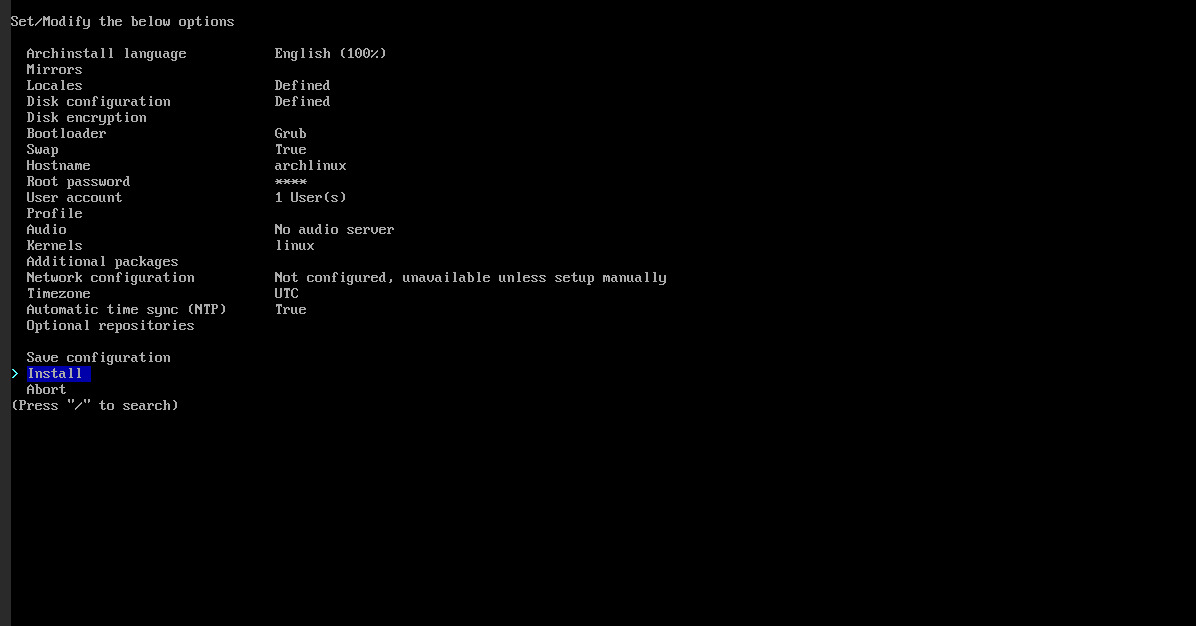
\includegraphics[width=0.8\textwidth]{38.jpeg} % Placeholder for Arch installation screenshot
    \captionof{figure}{Arch Linux Installation Process}
\end{center}
\begin{center}
\begin{center}
    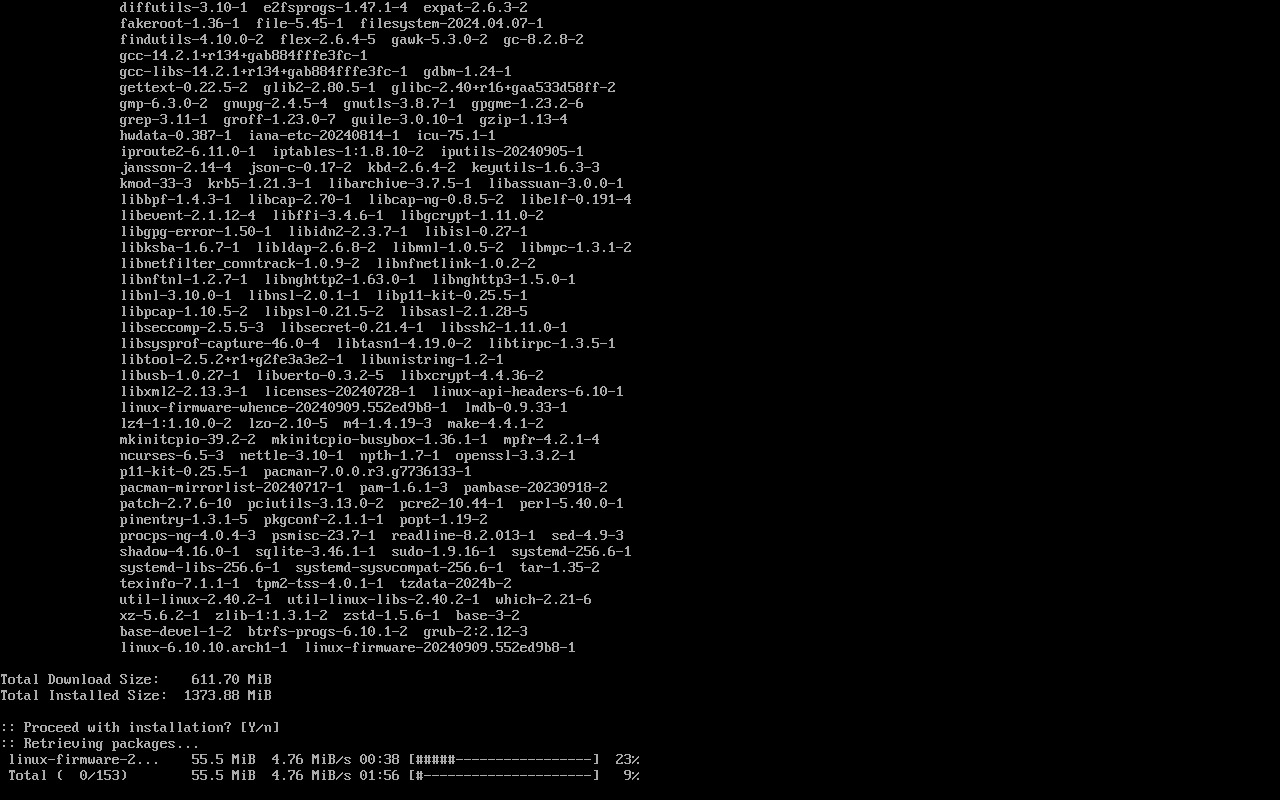
\includegraphics[width=0.8\textwidth]{ta.jpeg} % Placeholder for Arch installation screenshot
    \captionof{figure}{Arch Linux Installation Process}
\end{center}
    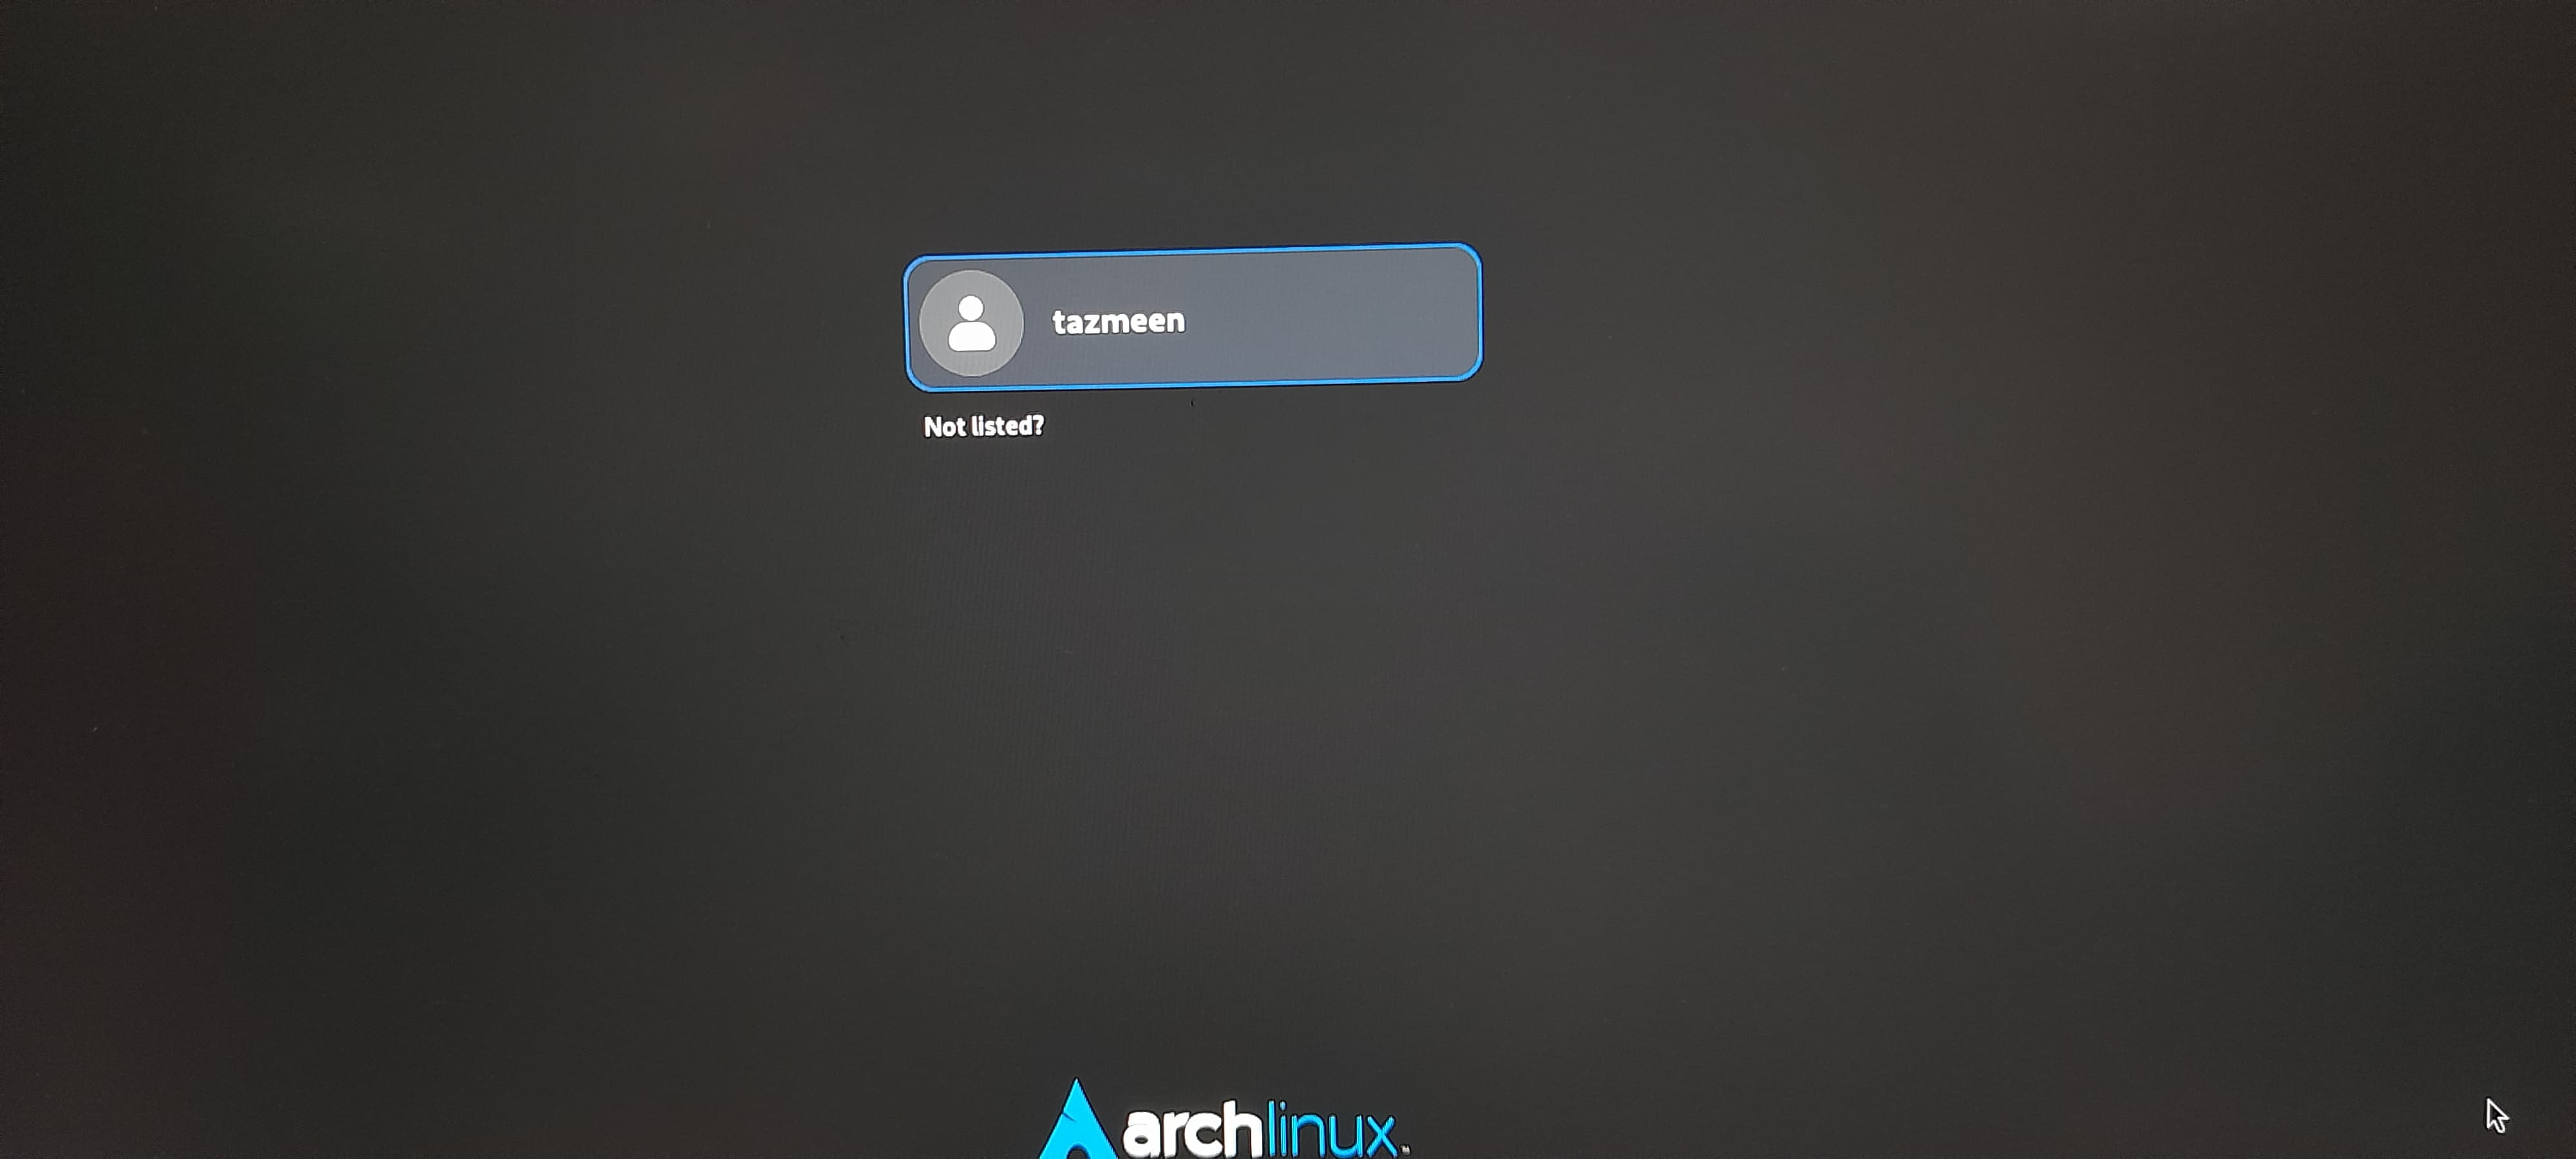
\includegraphics[width=0.8\textwidth]{xyz.jpeg} % Placeholder for Arch installation screenshot
    \captionof{figure}{Arch Linux Installation Process}
\end{center}
\begin{center}
    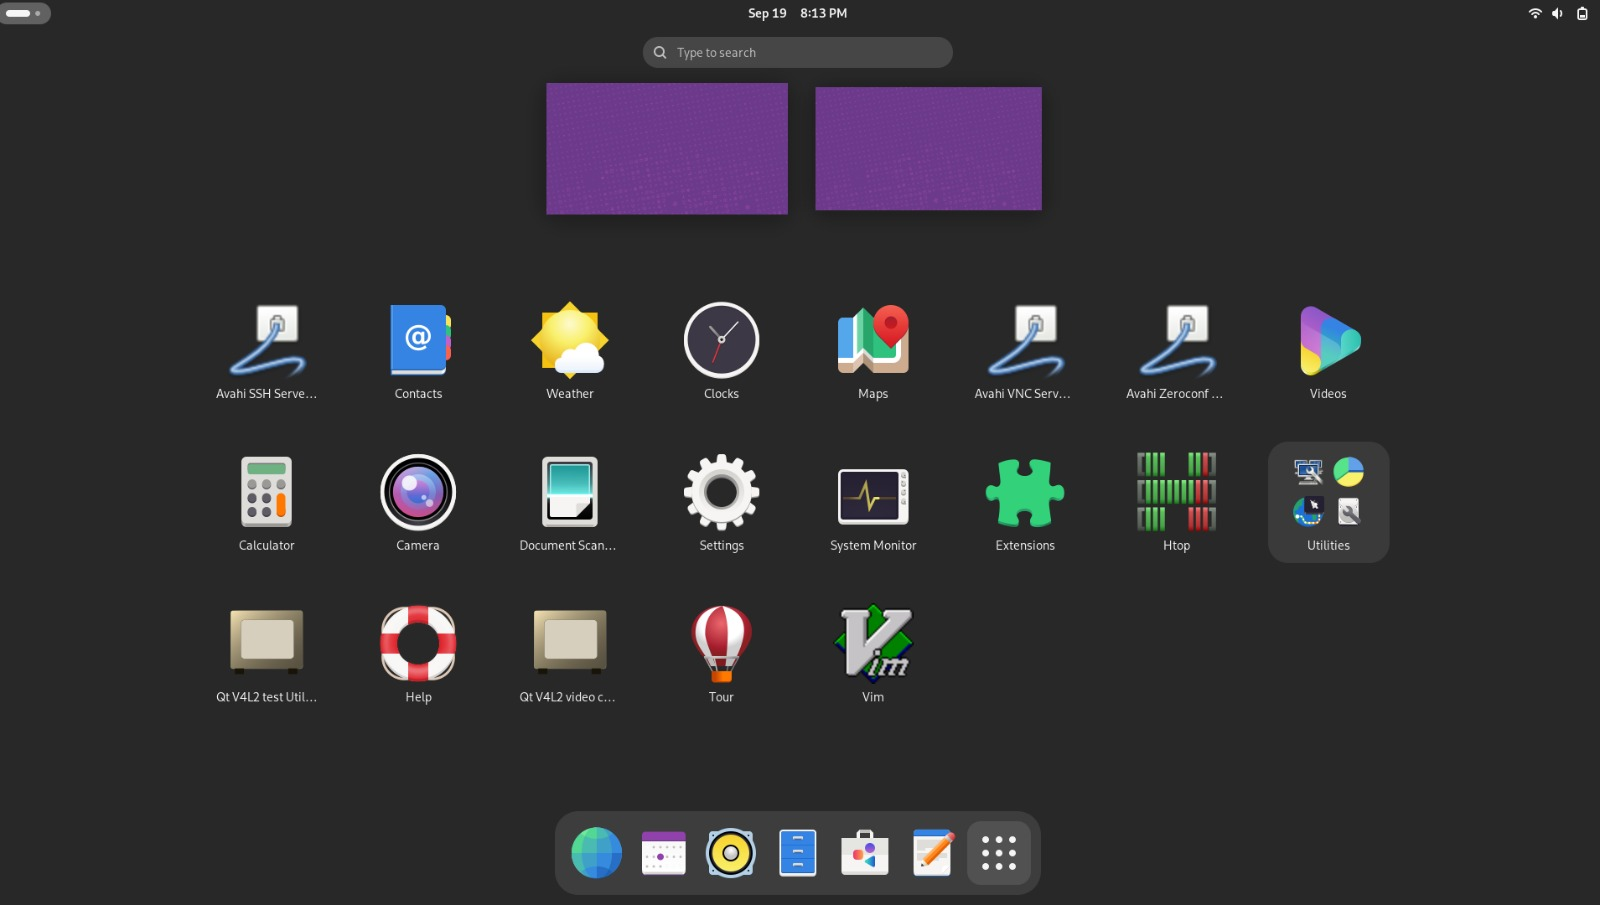
\includegraphics[width=0.8\textwidth]{z.jpeg} % Placeholder for Arch installation screenshot
    \captionof{figure}{Arch Linux Installation Process}
\end{center}
\begin{center}
    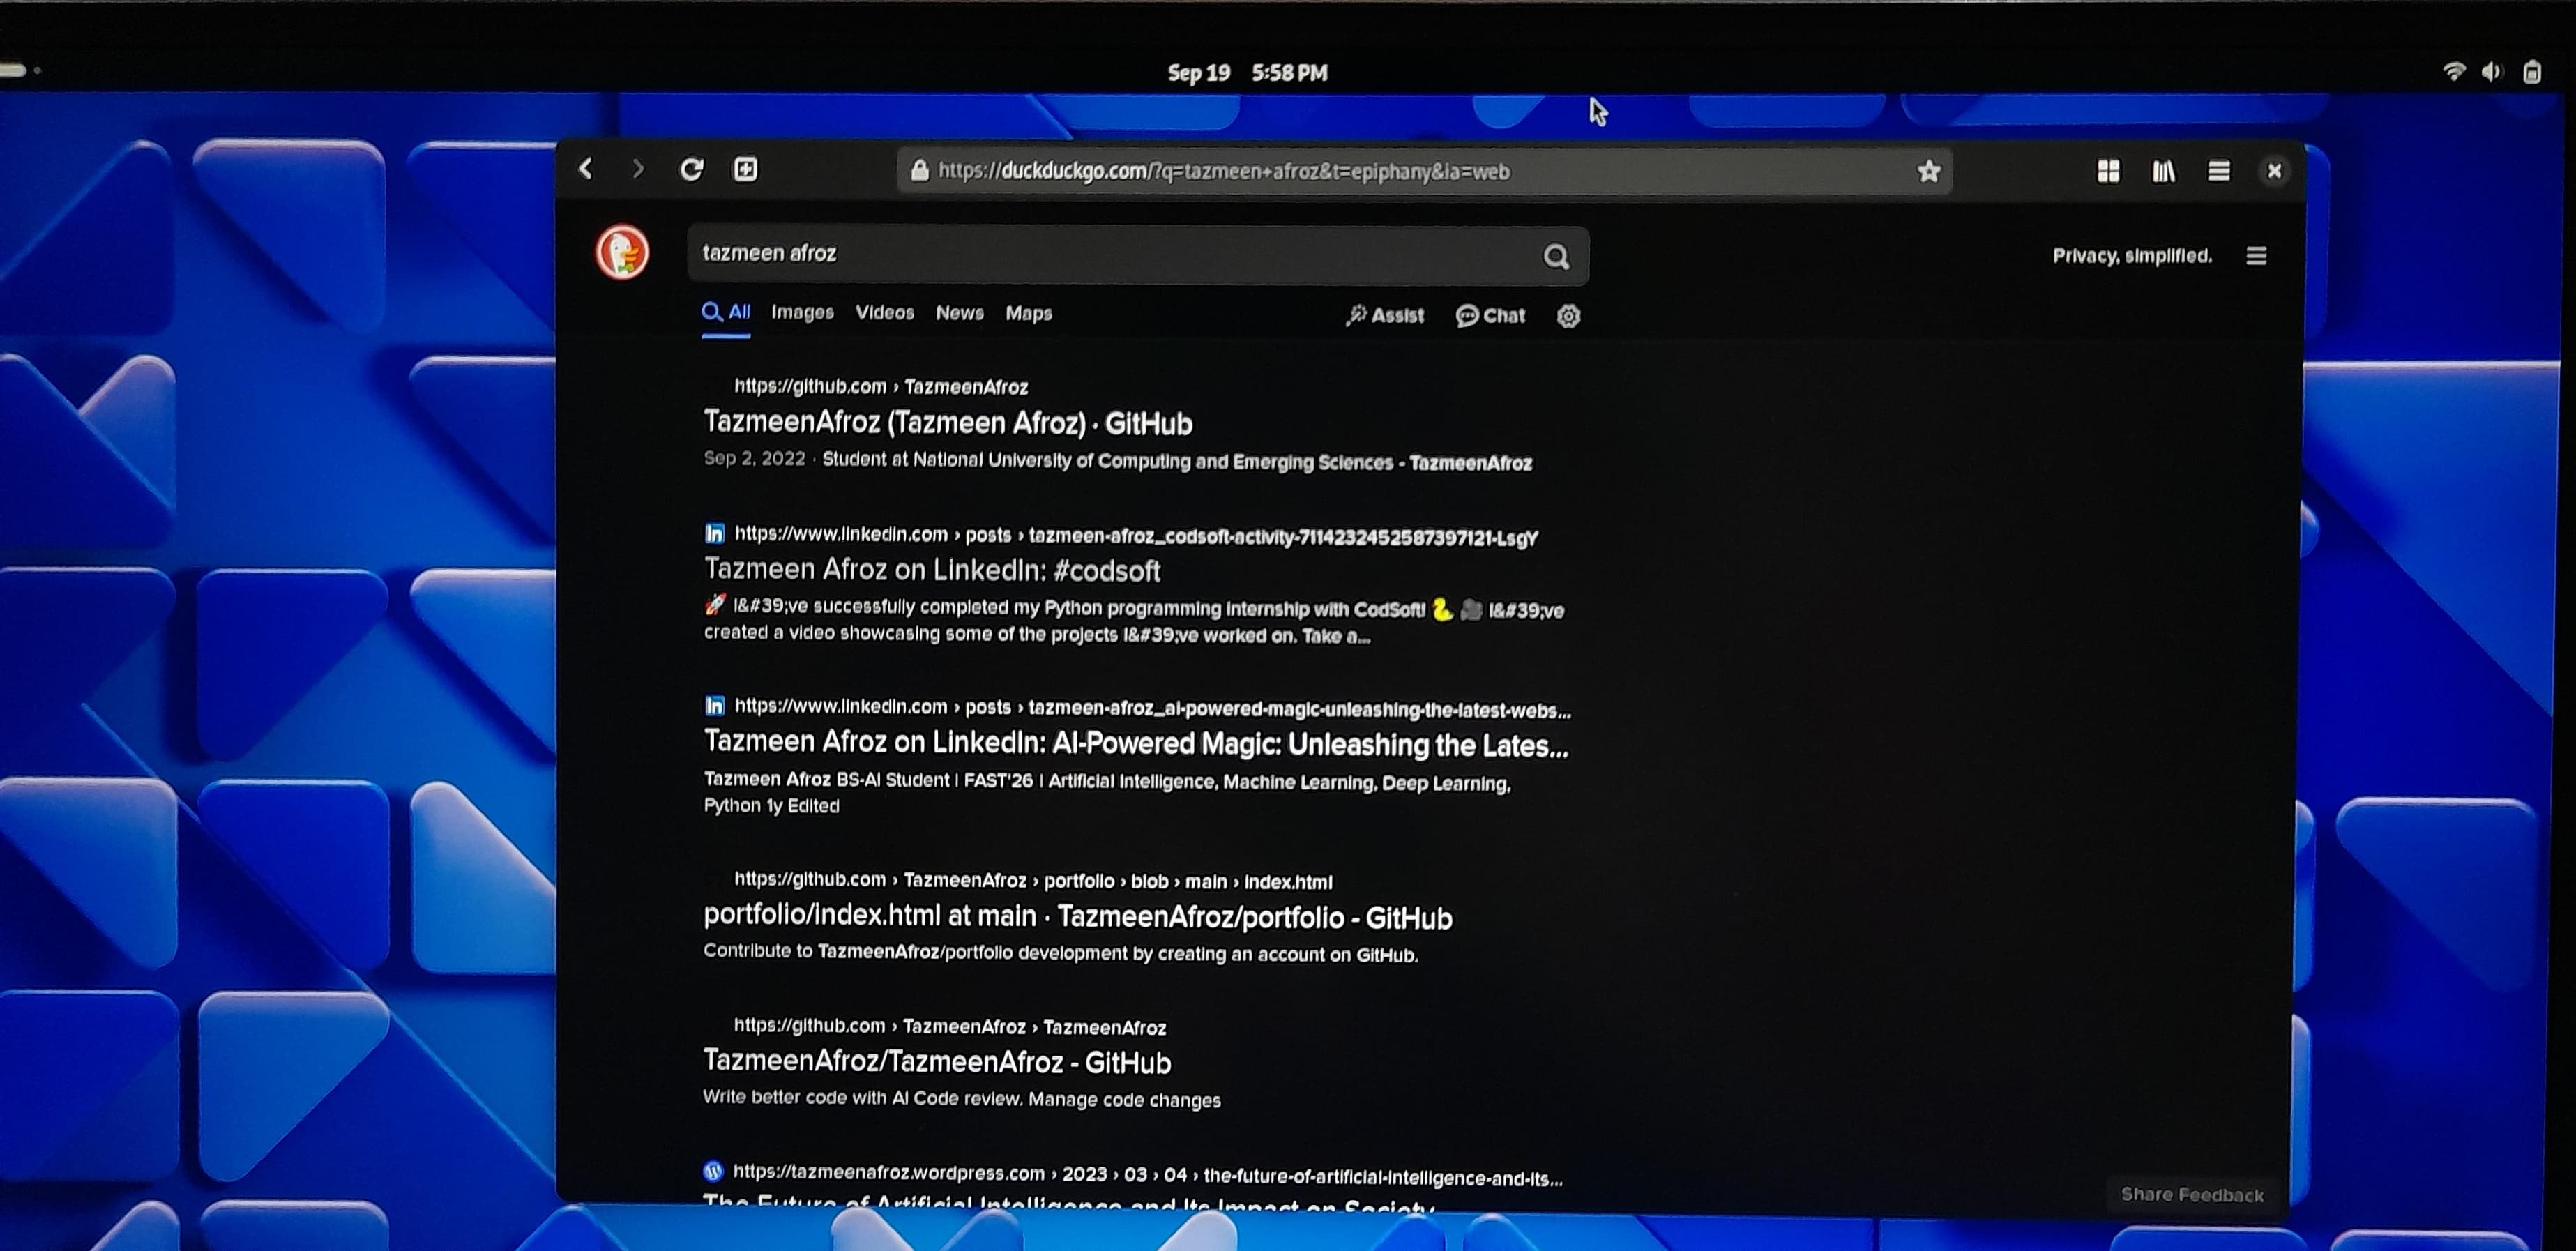
\includegraphics[width=0.8\textwidth]{k.jpeg} % Placeholder for Arch installation screenshot
    \captionof{figure}{Arch Linux Installation Process}
\end{center}
\subsection{Installing the GRUB Bootloader}
After installing Arch, set up the GRUB bootloader to manage all installed operating systems.

\section{Installing Ubuntu}
Finally, install Ubuntu on the remaining partition.

\begin{center}
    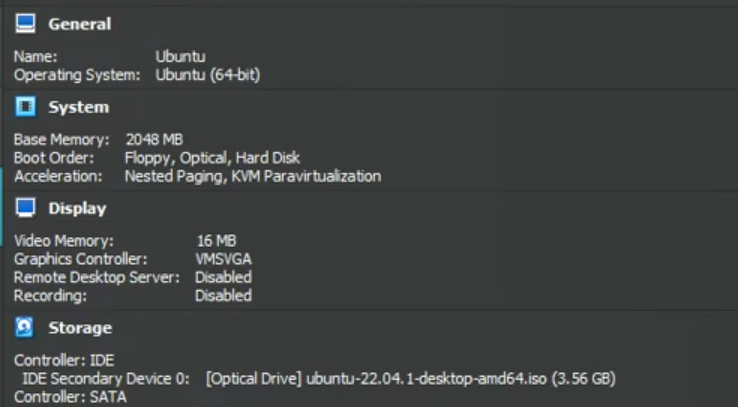
\includegraphics[width=0.8\textwidth]{a.png} % Placeholder for Ubuntu installation screenshot
    \captionof{figure}{Ubuntu Installation Process}
\end{center}
\begin{center}
    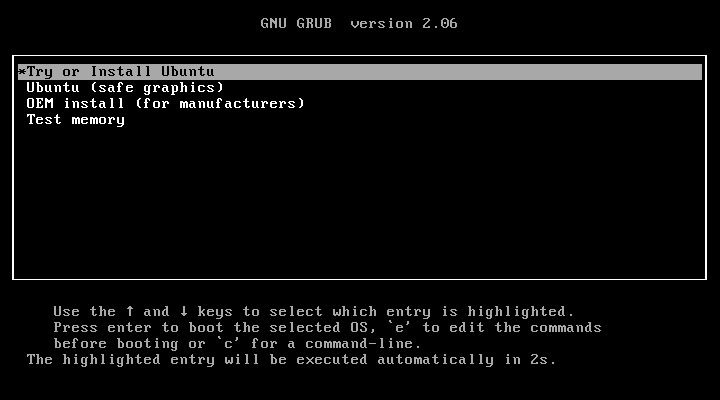
\includegraphics[width=0.8\textwidth]{39.jpeg} % Placeholder for Ubuntu installation screenshot
    \captionof{figure}{Ubuntu Installation Process}
\end{center}

\begin{center}
    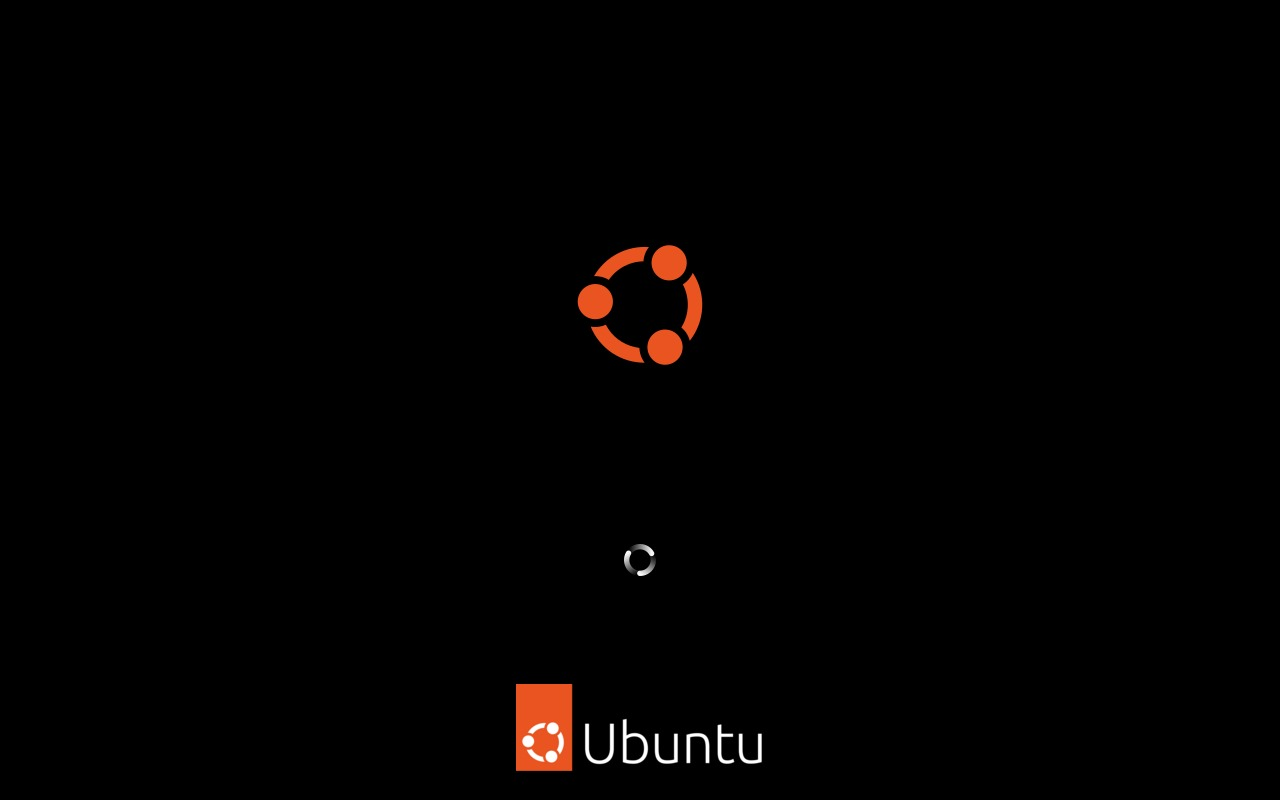
\includegraphics[width=0.8\textwidth]{40.jpeg} % Placeholder for Ubuntu installation screenshot
    \captionof{figure}{Ubuntu Installation Process}
\end{center}
\begin{center}
    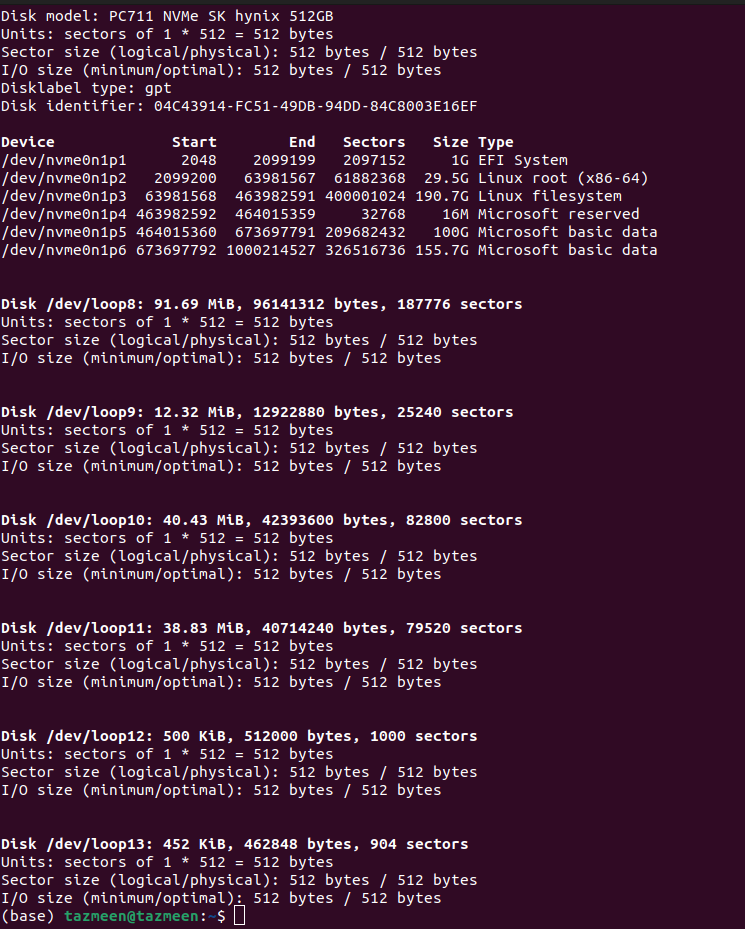
\includegraphics[width=0.8\textwidth]{41.png} % Placeholder for Ubuntu installation screenshot
    \captionof{figure}{Ubuntu Installation Process}
\end{center}

\section{Verifying the Triple Boot Setup}
After all installations are complete, reboot your system and check that the GRUB menu shows options for Windows 11, Arch Linux, and Ubuntu.

\begin{center}
    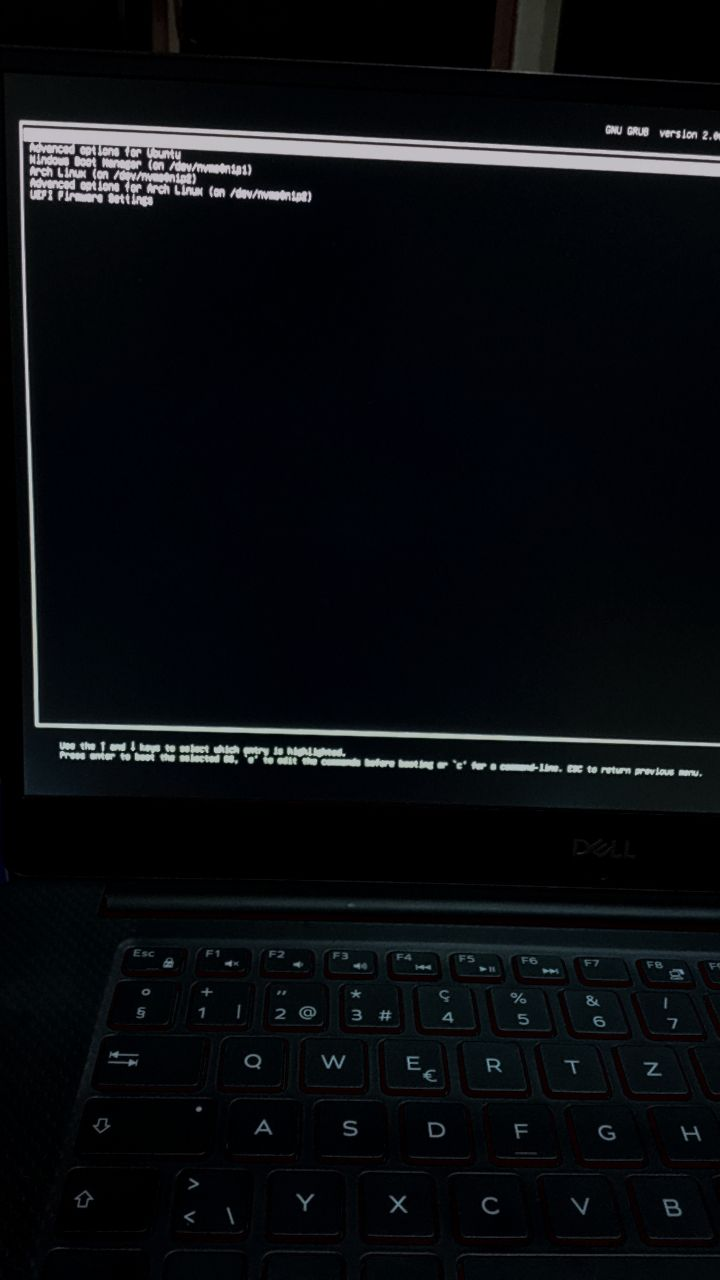
\includegraphics[width=0.8\textwidth]{ff.jpeg} % Placeholder for final GRUB screenshot
    \captionof{figure}{Final GRUB Menu}
\end{center}

\section{Conclusion}
This guide provided detailed instructions for setting up a triple boot system with Windows 11, Arch Linux, and Ubuntu on a virtual machine. By correctly configuring partitions and the GRUB bootloader, you now have a functional system with multiple operating systems.

\end{document}
